\chapter{Implementation}
\label{ch:15mc}

This chapter describes the work behind the envisioned platform, ``\textbf{15-Minute City}'', where each section starts with an overview of the problem, followed by a detailed list of available implementations for the problems introduce and finally the purposed solution to the problem.

The following chapter is split into multiple sections starting with \textbf{Scraping} (\ref{s:scraping}) details the design choices and implementation intricacies of the solution, while also highlighting some of the difficulties found. That section is followed by the \textbf{Microservices} (\ref{s:microservices}) each with their own challenges to overcome, such as communication and domain specific problems. To display all this details, a \textbf{user interface} was created, details which can be found in section \ref{s:user-interface}. At last \textbf{Monitoring}, in section \ref{s:monitoring} details how the system was monitored and why it was useful, which pairs perfectly with Testing chapter (\ref{ch:testing}), allowing the fine tuning of the application according to the information observed.
    
% In this chapter, we will present our proposed solution 15-Minute City, starting each section with a general overview of the problem, followed by a detailed list of available implementations and our solution to the problem. The first section, Scraping (\ref{s:scraping}) details the design choices and implementation intricacies of the solution, while also highlighting some of the challenges we had to overcome. This section is followed by the Microservices (\ref{s:microservices}, the backend that supports the entire application, explaining how they communicate, their functionalities and interesting problems related to each one. To present everything to the user an user interface was created, and details to such implementation lie in section \ref{s:user-interface}. Section \ref{s:monitoring} details how we monitor the system and why it was useful, which pairs perfectly with testing described in section \ref{s:testing}, allowing us to fine tune the application according to the data monitored.



\section{Scraping}
\label{s:scraping}

%\include{Chapters/04_RealEstateData}
%\chapter{Scraping}

% Resumir o capitulo aqui

%\subsection{Problem}
%\label{s:4_problem}
In most recent application, one of the most important components is data. As such, data classification is of utmost importance and each data source carefully selected. As a first step, we looke into some of the most common real-estate websites available in Portugal, compile into the following list:

\begin{itemize}
    \item \textbf{Idealista}: listing aggregator, fits all requirements but has advanced anti scraping mechanisms (i.e., captcha, ip blocking), as such it was avoided;
    \item \textbf{Imovirtual}: the second listing aggregator tried, provides reliable information that fits all criteria and is easy to scrape;
    \item \textbf{Remax}: It fits all requirements but unlike the previous websites, Remax is not a listing aggregator which results in a smaller number of listings;
\end{itemize}

Based on these platforms, we identified some of the core characteristics required to properly define a listing, and the following list represents the bare minimum listing detail required for the 15-Minute city platform.

\begin{itemize}
    \item \textbf{Location}: To be able to infer the distances between places having the location of each listing is mandatory. As such, these must include location names and coordinates;
    \item \textbf{Price}: It is one of the key limiting factors when searching for a new home, as such it is important to have the information available;
    \item \textbf{Size}: As pricing, it is relevant to understand the square meters of the house to decide if it is a good fit;
    \item \textbf{Bedrooms}: Number of rooms in each house excluding the kitchen and living room (following the Portuguese way of describing homes).
    \item \textbf{Commodities}: Perks associated with each house which may include: pools, garage, solar power, etc.
\end{itemize}

One of the most common occurrence between each website is the heavy reliance on Javascript, which makes them harder to scrape, one such example is the use of element rendering based on user interaction, where the host in orer to save bandwidth does not render the entire page until the user tries to use it. As such, specialized tools are required to simulate an user interacting with the application (e.g., scrolling down).

%With all of these in mind, we are now aware of what type of technologies we will need, and as such, the following section will go into detail of the tools at our disposal.

% Eescolher a informação necessária a extrair & fontes de informação
%The first obstacle was trying to understand the necessary data for the problem and, from there, how much of it is available. It was decided that the bare minimum information would be: Price, Location (Coordinates), Size (sqm), Bedrooms(T1,T2...) and Commodities. Therefore, while looking for sources, only the ones with that information would be considered. If a source also includes extra information such as the floor or textual descriptions of the house, the data is stored, which may allow for further analysis in the future, with techniques such as NLP. 

%Currently, there is several real estate companies that list AD information as required, the following websites were picked: Imovirtual, Idealista e Remax.

%As most of these websites are modern and rely heavily on Javascript, they require extra steps to allow data extraction, one example of those cases, is the use of element rendering based on user interaction, allowing the host do save bandwidth by not rendering the entire page. As such specialized tools are required to simulate an user interacting with the system (e.g., scrolling down).

% Falar da necessidade de obter dados de localizacao


\subsection{Solution}
\label{s:scraping-solution}

By defining the core characteristics necessary to describe each listing and analysing the needs of the systems, the first stop must be to defined the data model, which can be seen in Appendix \ref{apx:er-estates}. The model consists of two main categories: listing information and geographical data. The following listing contains a brief description of the main tables and their purposes:

\begin{itemize}
    \item \textbf{Estate}: listing information that describes each specific estate;
    \item \textbf{Feature}: possible features of a house such as garage, pool, etc;
    \item \textbf{Source}: know sources of where to scrape estate data;
    \item \textbf{Ad Status}: state of the listing;
    \item \textbf{Crawl History}: crawling occurrences of each listing;
    \item \textbf{Price History}: price evolution of a listing;
    \item \textbf{Location}: estate coordinates extracted from the scraped listing and associated with an estate;
    \item \textbf{Parish}: contains information that describes each civil parish, as well as their geographical properties (shape and centroid);
    \item \textbf{Municipality}: information that describes each municipality, as well as their geographical properties (shape and centroid);
    \item \textbf{District}: contains information that describes each district, as well as their geographical properties (shape and centroid);
    \item \textbf{Country}: information that describes each country, as well as their geographical properties (shape and centroid);
    \item \textbf{NUTS1}: NUTS \footnote{\textbf{N}omenclature of \textbf{T}erritorial \textbf{U}nits for \textbf{S}tatistics: is a geocode standard for referencing the subdivisions of countries for statistical purposes} 1 information and geographical properties (shape and centroid);
    \item \textbf{NUTS2}: NUTS 2 information and geographical properties (shape and centroid);
    \item \textbf{NUTS3}: NUTS 3 information and geographical properties (shape and centroid).
\end{itemize}

To store geographical data we opted to use a spatial database, which extends general purpose databases by providing spatial indexing and support for spatial queries. With it, it was possible to store geographic objects in vector formats, which allows effective and efficient management of geospatial data. Even though there were multiple solutions available to save this type of data, we chose PostGIS~\footnote{See: \url{https://postgis.net/}} a PostgresSQL extension, due to previous working experience.

This data was obtained through the \textit{OpenDataSoft}~\footnote{See: \url{https://www.opendatasoft.com/}} platform, which since then has been removed. While it was available it was possible to obtain the following portuguese data: districts, municipalities, parishes, NUT 2 and NUTS3. The geographical information pertaining the country and NUT1 information was not available. To fix it, we used spatial queries to intersect all the districts and merged into one polygon, representing the country of Portugal.

To extract the information from the chosen data sources, a scraping pipeline was first defined, as depicted in Fig. \ref{fig:scraping-architecture}. The goal was to create a solution that could easily be scaled to process different number of requests and also support the addition of new real estate websites to the pipeline.

\begin{figure}[H]
	\centering
	\begin{tikzpicture}
        \node{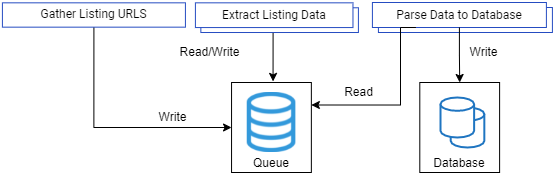
\includegraphics[width=1\linewidth]{Chapters/img/4_realEstateData/scraping-pipeline.png}};
        \node[xshift=-5cm, yshift=3cm, fill=white, circle, draw=gray]{1};
        \node[xshift= 0cm, yshift=3cm, fill=white, circle, draw=gray]{2};
        \node[xshift= 5cm, yshift=3cm, fill=white, circle, draw=gray]{3};
    \end{tikzpicture}
	
	\caption{Scraping architecture}
	\label{fig:scraping-architecture}
\end{figure}

This solution has three distinct sections, represented by three columns in Fig.~\ref{fig:scraping-architecture} where each has a different purpose:

\begin{enumerate}
    \item Responsible for gathering URLs and sending them to a queue named after their data source (e.g., remax-queue);
    \item Receive an URL from the queue, scrape the information from the listing and send it to the queue;
    \item Process the listings received by cleaning it and validating the information, then write it on the database;
\end{enumerate}

For the \textbf{first section}, it was necessary to obtain a base \acrshort{url} to act as a starting point for the scraper, which has to lead to a page with multiple estate listings. The goal was to get \acrshort{url}s that could provide as much data as possible, reducing the amount of pages scraped and avoiding overloading the source, while also trying to obtain listings for the entire country off of one \acrshort{url}. Which led to the following base \acrshort{url}s:

\begin{itemize}
    \item \textbf{Imovirtual}: https://www.imovirtual.com/comprar/apartamento/ ?search[order]= created\_at\_first:desc\&search[created\_since]=3 \&nrAdsPerPage=72
    \item \textbf{Remax}: https://remax.pt/comprar? searchQueryState= {"regionName":"", "sort": {"fieldToSort": "ContractDate","order":1}, "page":1, "mapIsOpen":false, "publishDate":7, "businessType":1, "listingClass":1}
\end{itemize}

For \textbf{Imovirtual}, to obtain the entire country with a single query, all it required was the deletion of the flag $&locations[0][region\_id]=ID$ and to obtain the maximum number of pages we had to include the flag \url{nrAdsPerPage=72}, being 72 the maximum number of listings possible to retrieve. In the \textbf{Remax} \acrshort{url}, we had to delete the information associated with the \textbf{\textit{regionName}} flag and send it as an empty string, as seen in the previous example. This way it was possible to retrieve the entire country all at once, however unlike Imovirtual it was not possible to tune the number of listings shown per page.

The third most important parameter in the \acrshort{url}s was the flag that allowed to query only listings published within certain time intervals. This way it was possible to schedule autonomous scraping through the use of CRON jobs, as it is possible to ensure we will retrieve all data published within the last days. Both of them impose no restrictions, as such it was possible to obtain the information for the entire year, but we decided to scrape them once a week to keep data fresh and only once week to not overload the hosts. The following flags were used: Remax -- \url{"publishDate":7} and Imovirtual -- \url{search[created_since]=7}.

To scrape the websites we opted to use \textbf{Scrapy} \footnote{See: \url{https://scrapy.org/}}, an established framework for large scale web scraping that provides all the tools to efficiently extract, process and store data while also being ready to be easily scalable and already organized into independent modules. One of the main workhorses of Scrapy are \textbf{Spiders}, the classes used to defined the custom behaviour for parsing the page(s). 

With the base \acrshort{url}s defined, we instructed the spider to process each page with the use of \acrshort{xpath}, which allowed us to extract the listings \acrshort{url}s, and send them to the queue. 

To provide a scalable experience, we opted to use a remote queue to act as an intermediary between all the components, as Scrapy was already prepared to use \textbf{Redis} and it was appropriate to the problem, it was chosen for this solution. Each item, was sent to a specific key according to their origin (\textit{remax:items} and \textit{imovirtual:items}), they were split into different categories as each website as different processing needs. After extracting all the listings from the first

The \textbf{second section} is responsible for extracting the actual listing data from each URL, which is obtained from the queue, and as before the data is extracted with the help of XPATH expressions. But, as stated previously, these websites only load elements through user interaction. To deal with this used \textbf{Selenium}, a framework commonly used for web application testing that has tools to automate and simulate human browsing behaviour. This was used in our advantage, by making the website think it is interacting with a user and allowing us to scrape the page content. This was possible by using the \textbf{Selenium Webdriver API} in conjunction with a browser driver (such as ChromeDriver for Google Chrome) and defining programmatic interactions through its library methods.

Imovirtual had this problem, where to extract the map coordinates it required the user to scroll down the entire page to load the map that showed the estate location.

The listing data is extracted, and mapped into a JSON composed of the following fields:

\begin{itemize}
    \item \textbf{URL} - URL of the ad;
    \item \textbf{Source} - Name of origin;
    \item \textbf{Price} - The current price of the estate;
    \item \textbf{Title} - Title of the ad;
    \item \textbf{Location} - Location name (district, municipality, parish), amount of fields varies based on the information provided and source;
    \item \textbf{Overview} - Must have estate information such as: square meters, floor, energy efficiency, bathrooms, etc...;
    \item \textbf{Description} - Textual description provided on the ad;
    \item \textbf{Features} - Extras included in the house (garage, lift, etc...);
    \item \textbf{Coordinates} - Longitude and Latitude;
    \item \textbf{Source Information} - Information provided by the source such as: id, date of creation and date of last modification.
\end{itemize}

Photos were excluded in the extraction as they were considered off limits as stated in the \textit{robots.txt} rules for each website. Each object is then sent into the queue \textit{general:processing}, which is now the same queue independent of source, so they can be processed by the next section of the pipeline. \\

During the \textbf{third section}, the items are now ready to be processed and inserted in the database. After the item is read from the queue, it gets sorted by the source name, and since each source has a corresponding function with the same name, it is possible to use Python reflection to call the appropriate function to process each item. This process can be observed in the following code: \\

\begin{lstlisting}[language=Java, caption={Snipet of code responsible for selecting the appropriate path for each item}, captionpos=t]
# Get JSON from the queue
json_str = self.redis.queue.blpop(self.queue_name)
# Extract item properties
item = json.loads(json_str[1].decode())['_values']
# Get the appropriate function from the source name received
method = getattr(self, item['source'], lambda: "Invalid source.")
# The method instantiates the required class to process the item 
selected_class = method(item, db_host, db_port)
# Start the cleaning process and obtain the final item
item = selected_class.main()
# Start process to insert onto the database
self.insertDB(item, selected_class)
\end{lstlisting}

During the event that occurs on line 10 of the previous code, all elements are processed which includes: removal of HTML tags, weird spacing, symbols (``€'' or ``$m^2$''), items in Portuguese are translated to English, etc. One of the most common problems were related to the locations, as due to user error, a large portion of the written locations described in the listings did not match the coordinates, sometimes even being in different continents, as such only items that had matching locations and coordinates were added to the database.

To validate this information, the coordinates obtained from the ad were intersected with the geographical information stored in the database, with the help of the ST\_WITHIN function from PostGIS, where we managed to obtain the real location name composed of: the parish, municipality, district, and country; and compare it with the information previously scraped.

During the fourth, and last step, items were stored in the database with the help of SQLAlchemy, an \acrfull{orm} -- a python library that translates Python objects to tables in SQL databases and automatically converts function calls to SQL statements (i.g., SQL \textit{WHERE} functions corresponds to filter\_by()). 

Since it is bound to happen that listings may appear multiple times, before each insertion, it is necessary to verify if the listing already exists in the database, if it does not, the object is created and promptly inserted. If they do exist, the items are instead updated as items such as house features, or textual descriptions may have been changed since the last time. Given that this process involves multiple tables and to ensure that data stays consistent all of this process is wrapped in a transaction that rolls back if any of the steps fails.

Due to the nature of the data, and its time relevancy (crawl history), every date and time reference is converted to the timezone of the server location (Europe/Lisbon) and converted to the ISO 8601 format (YYYY-MM-DDTHH:MM:SS), ensuring that everything is now consistent. \\

\subsubsection{Infrastructure}
\label{sss:scraping-infrastructure}

To deploy the previous pipeline, each process represented in Fig. \ref{fig:scraping-architecture} was containerized with Docker, always trying to keep the images as small as possible. All of them included the official Python image as our base image, instructions to copy our work directory and the dependencies installation. For processes that required selenium, we had to install chrome which is used by selenium to interact with the pages, which required the following configuration in the image dockerfile:

\begin{lstlisting}[float, language=Java, caption={Dockerfile configuration of the scrapper}, captionpos=t]
# Adding trusting keys to apt for repositories
RUN wget -q -O - https://dl-ssl.google.com/linux/linux_signing_key.pub | apt-key add -

# Adding Google Chrome to the repositories
RUN sh -c 'echo "deb [arch=amd64] http://dl.google.com/linux/chrome/deb/ stable main" >> /etc/apt/sources.list.d/google-chrome.list'

# Updating apt to see and install Google Chrome
RUN apt-get -y update
RUN apt-get install -y google-chrome-stable
# Installing Unzip
RUN apt-get install -yqq unzip

# Download the Chrome Driver
RUN wget -O /tmp/chromedriver.zip http://chromedriver.storage.googleapis.com/`curl -sS chromedriver.storage.googleapis.com/LATEST_RELEASE`/chromedriver_linux64.zip

# Unzip the Chrome Driver into /usr/local/bin directory
RUN unzip /tmp/chromedriver.zip chromedriver -d /usr/local/bin/
\end{lstlisting}

Given that each process now has their docker image, they could now be launched as Kubernetes deployments. \\

As the data extracted here is the most important to the project, we have tried to ensure that it would always be available. As such, the postgres cluster was deployed in a master-slave configuration with the help of \textbf{Bitnami PostgreSQL High-Availability}, a pre-existing package of \acrshort{k8s} configurations (helm charts) to deploy the cluster with minimal configuration.

Primary-secondary replication enables data from one database server (primary) to be replicated to one or more database servers (secondary). This way, database servers can work together to allow a secondary server to take over quickly if the primary server fails (high availability) with the use of the fail-over mechanism, or to allow several computers to serve the same data (load balancing).

\begin{figure}[H]
	\centering
	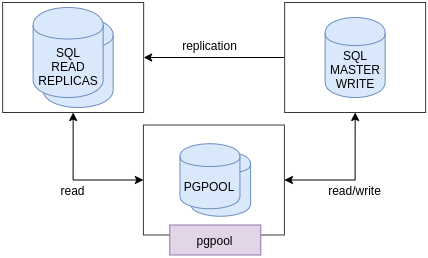
\includegraphics[width=0.7\linewidth]{Chapters/img/4_realEstateData/BD_Estates.png}
	\caption{Estates PostgreSQL architecture (Primary-Secondary)}
	\label{fig:bd-estates}
\end{figure}

These standby databases will remain synchronized with the primary node. The replication between the primary and the secondary nodes can be made via SQL statements or via internal data structure modifications. As this project used PostgreSQL, a stream of write-ahead log (WAL) records were used to keep the standby databases synchronized. WAL is a standard approach to transaction logging, where the main idea is that changes to the database must be written only after those changes have been logged. 


To effectively ensure high availability, it is not enough to have a primary-seconary architecture, so it is necessary to enable some automatic form of failover and since postgres does not have a default failover solution, PGPool-II was used. In this context, failover means automatically detaching PostgreSQL backend node which is not acessible by Pgpool. This inaccessibility is confirmed by regularly checking node healthiness, which it does by trying to connect to the node. When it happens, since the standby database contains all data of the main server, it can use it to become the new primary server. Unfortunately, even with all of this solutions data loss may still happen, since errors can occur in the middle of write operations and the logs for those operations may not had the time to be written. The cluster is then exposed to the outside via a \acrshort{k8s} service, represented with purple in Fig. \ref{fig:bd-estates}.

\begin{lstlisting}[float, language=Java, caption={Cron job specification to launch the scrapping jobs}, captionpos=t, label={lst:cronjob-configuration}]
apiVersion: batch/v1beta1
kind: CronJob
metadata:
  name: py-imovirtual-data-scale-up-cronjob
  namespace: py-scrapping
spec:
  successfulJobsHistoryLimit: 1
  failedJobsHistoryLimit: 1
  schedule: "0 0 * * 1" #Meia noite todas as segundas
  jobTemplate:
    spec:
      activeDeadlineSeconds: 180
      template:
        spec:
          serviceAccountName: scheduled-autoscaler-service-account
          containers:
          - name: py-imovirtual-urls
            image: biole/imoveis_scrapping:latest
            command: ["/bin/sh", "-c"]
            args: ['cd src; scrapy crawl imovirtual']
            resources:
              limits:
                memory: "400Mi"
                cpu: "300m"
            ports:
              - containerPort: 80
              - containerPort: 443
              - containerPort: 30036 
              - containerPort: 32658
          restartPolicy: Never
\end{lstlisting}


To handle the calendarization, scraping jobs were launched with \acrshort{k8s} using their own specification for \textbf{CronJobs}, as shown in listing \ref{lst:cronjob-configuration}. Within this configuration it is possible to configure the scheduling, so it occurs every seven days (every Monday at midnight), specify the container to run and arguments should it be run on. Additionally the pod resource usage was also configured, in this scenario the Memory and CPU usage was limited, letting the cluster know to never go below this values.




%As this section of the application contains the most important data , we have tried to ensure that it would always be available.
%As this was the most important section of data from the application, we tried to ensure it would always be safe and available.




% Falar aqui que sao dados importantes então base de dados tem backup, replicada, etc....


% Falar da infrastrutura necessária para ter tudo a funcionar (kubernetes): postgres, redis, python scripts
%% Falar dos recursos necessários (ex: foram atribuidos 200mb para o script X, 300mb para o y?)




\section{Backend}
\label{s:microservices}

%\chapter{Microservices}
%\label{ch:microservices}

Upon extracting the real estate data and storing it, it is now necessary to make the data available. This aligns with the goal of creating a cloud application that follows a microservice architecture, where each service is small and focused, so each can be an independent application.

As stated previously, containers are easier to manage when compared to virtual machines, and as they are lightweight, they become an invaluable tool to help us deploy our microservices. However, given that we are bound to have multiple containers, it becomes hard to manage each one independently, as such, we also require a tool to automate the orchestration of all these containers.

Having services broken up into smaller chunks, gives the added benefit of easier failure isolation, as it allows for faster recovery by discovery problems faster. However, by splitting everything into smaller pieces, it becomes a challenge to route traffic between and to services. A way to solve this is through the use of an API Gateway, a special server which acts as the only entry point to the microservices, usually located on the system boundary, encapsulating the internal aspects of the system. One of the drawbacks is that it becomes a single point of failure for the system, as all communication is done through it, but even with this compromise, the benefits outweigh the risks.

One of the characteristics of the microservices architecture is that services are loosely coupled, and one of the ways to achieve this is by assigning a different database to each service. This loose coupling also complicates the communication, however, as microservices are language-neutral, there also language-neutral ways of communicating, such as HTTP via Rest to communicate with the exterior and messages for inter-service communication. 

\subsection{Solution}
\label{ss:backend-solution}

Based on the objectives and proposed solution described previously, we defined what services would be necessary to obtain our application \acrfull{mvp}, and as such the following service definitions were drafted:

\begin{itemize}
    \item \textbf{Estate}: estates (or listings) are considered the main component of the application and as such a microservice to manage it, is required. As such, it is responsible for all information related to the estates (e.g., estate coordinates, price);
    \item \textbf{Parameter}: From the idea of the social functions of the 15-minute city, the Parameter service was born, responsible for dealing with all the information related to points of interest;
    \item \textbf{User}: To classify each house according to each specific user, it was necessary to create a service to manage user information (e.g., personal preferences);
    \item \textbf{Authentication}: To have users, they need to be capable of authenticating and registering themselves within the application; 
    \item \textbf{Metrics}: The relation between the user, estates and parameters (index) is dealt with within the Metrics microservice. It is also used to manage all the metrics associated with each zone;
    \item \textbf{Search}: Since the user needs to search for locations of interest within the application, a service was created to support the search bar.
\end{itemize}

These services in conjunction with the previous storage solutions studied, let to the creation of the architecture presented in Fig. \ref{fig:microservices-overview}.

\begin{figure}
	\centering
	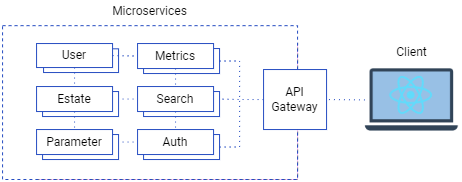
\includegraphics[width=1\textwidth,clip,trim=0 0 0 0]{Chapters/img/backend/ArqOverview_Focused.png}
    \caption[Microservice diagram]{Diagram of available microservices with client requests being funneled through the API Gateway} 
    \label{fig:microservices-overview}
\end{figure}

Each service has its own container, and as the main technology used to implement each service is Java we tried to facilitate the building of Docker images by using \textbf{JIB}~\footnote{See: \url{https://github.com/GoogleContainerTools/jib}}, a tool from Google that builds optimized Docker images without having to depend on a Docker daemon. To deploy them in the \acrshort{k8s}, a Kubernetes service and deployment are also built, with a configuration similar to the one shown in Listing \ref{lst:k8s-deployment}. 

The main takeways from this deployment is how we have organized our kubernetes through the use of namespaces, in this case, all of our backend services are under the namespace \textit{backend}. Followed by the pod configuration each ditactes how many pods will be deployed (number of \textit{replicas}), their names, what docker image to use and from where to pull it, the assigned resources and finally, how to deal with cases of failure (restartPolicy) such as crashes.

\begin{lstlisting}[float,caption={[Microservice Kubernetes deployment configuration]{Example of a \acrshort{k8s} deployment configuration in YAML for a microservice}}, label={lst:k8s-deployment}, captionpos=t]
kind: Deployment
apiVersion: apps/v1
metadata:
  name: be-account-deployment
  namespace: backend
spec:
  replicas: 1
  selector:
    matchLabels:
      app: be-account
  template:
    metadata:
      labels:
        app: be-account
    spec:
      containers:
        - name: be-account
          image: biole/account:latest
          imagePullPolicy: Always
          resources:
            limits:
              memory: "300Mi"
              cpu: "1000m"
          ports:
            - containerPort: 80
      restartPolicy: Always
\end{lstlisting}

In the service configuration, as shown in Listing \ref{lst:k8s-service}, once again we set it up under the backend namespace and configure its type, NodePort, that assigns a static port from a range specified between 30000 and 32767, which makes the service now accessible from outside the cluster. This port can also be manually assigned, as we have done in our configuration. Each service has a port assigned in its spring configuration, for this case its 8083, which is then exposed in \acrshort{k8s} through the port 31003.

\begin{lstlisting}[float, caption={YAML configuration of a Kubernetes service}, label={lst:k8s-service}, captionpos=t]
kind: Service
apiVersion: v1
metadata:
  name: be-account-service
  namespace: backend
spec:
  type: NodePort
  ports:
    - port: 8083
      targetPort: 8080
      protocol: TCP
      nodePort: 31003
  selector:
    app: be-account
\end{lstlisting}

With the increasing number of services, it became difficult to remember and keep track of all existing ports, which was one of the many reasons that led to the implementation of an API Gateway, as seen in Fig. \ref{fig:microservices-overview}. With it, it is now possible to assign URIs to the services, facilitating the access from the frontend as 10.62.73.47:31003 now becomes 10.62.73.47/v1/authentication. Our implementation of an API gateway was done through the use of NGINX~\footnote{\url{https://www.nginx.com/}}, a snippet of the required configuration can be seen in the Listing \ref{lst:nginx-api-gateway}.

It also possible to observe in Fig. \ref{fig:microservices-overview} that the API Gateway acts as a single entry point to the system. Even though the possibility of becoming overloaded with requests exists, the way it simplifies the system overshadows those defects. By having an API Gateway it becomes unnecessary to know the ports of each service, as we can call it through a predefined URI. It also allows us to deal with authentication at this level, this way it is not necessary to verify if the user is authenticated beyond the gateway.

\begin{lstlisting}[float, caption={NGINX API Gateway snippet}, label={lst:nginx-api-gateway}, captionpos=t]
server {
    listen 80;
    server_name 10.62.73.47;

    location /v1/authentication/ {
        proxy_pass http://10.62.73.47:31003;
    }
    ...
}
\end{lstlisting}


\subsubsection{Authentication}

The authentication is supported by \textbf{AWS Cognito}~\footnote{\url{https://aws.amazon.com/cognito/}}, an Amazon platform that provides authentication, authorization, and user management for applications, it allows the user to sign in with credentials or through third party platform such as Facebook and Google. Through the use of Cognito Java \acrshort{api} we managed to create and expose through a Spring Boot \acrshort{api} the following functionalities available at /v1/auth:

\begin{enumerate}
    \item \textbf{login} (POST: /login): authenticate user with the provided credentials;
    \item \textbf{create user} (POST: /create\_user): create a new account by providing an username and an email, a temporary password is sent via email to complete the registration;
    \item \textbf{username lookup} (POST: /username\_lookup): recover the username registered by providing the email used during registration;
    \item \textbf{change password} (POST: /change\_password): alter the provided password by introducing the current password and the new password, the method implementation also accepts as input the type of password change to distinguish between freshly created accounts that have not logged in yet and normal accounts;
    \item \textbf{forgot password} (POST: forgot\_password): if the user forgets his password he can provide the registered username and code will sent to the email associated with the account;
    \item \textbf{reset password} (POST: reset\_password): after the user receives his code for password recovery from the last step, the element can be introduced along with his new password to change it; 
\end{enumerate}

Cognito upon sign-in returns a \acrfull{jwt} which is a JSON encoded representation of a claim(s) that can be transfered between two parties. This claim is digitally signed by the issuer of the token, and the party receiving this token can later use this digital signature to prove the ownership of the claim. This claims are used to provide authentication to the party receiving the token.

\begin{lstlisting}[float, caption={Route with authentication}, label={lst:nginx-api-gateway-auth}, captionpos=t]
location /v1/search/ {
        auth_request /auth/query_auth;
        proxy_pass http://10.62.73.47:31004;
}

location /auth/query_auth {
    proxy_pass http://10.62.73.47/v1/aws/auth/validate-jwt;
    proxy_pass_request_body off;
    proxy_set_header Content-Length "";
    proxy_set_header X-Original-URI $request_uri;
}
\end{lstlisting}

In this application, upon sign in each request includes the token associated with the logged-in user, granting him access to the platform by proving their identity. To validate the claim in every protected route we used the \textit{ngx\_http\_auth\_request\_module} module from NGINX, which implements client authorization based on the result of a subrequest, if the subrequest returns a 2xx response code, the access is allowed. If it returns 401 or 403, the access is denied with the corresponding error. Any other response code is considered an error. This implementation can be seen in the Listing \ref{lst:nginx-api-gateway-auth}, where search performs a subrequest to an endpoint implemented in the authentication microservice.

Since the request originates in Cognito, it also has to be validated with the corresponding information provided from AWS, in this case in the form of a public \acrfull{jwk} located in \textit{https://cognito-idp.{region}.amazonaws.com/{userPoolId}/.well-known/jwks.json.} (\textbf{userPoolId} parameter represents the user directory in Cognito created for this application). With this key it is now possible to verify the signature, as shown in Listing \ref{lst:auth-endpoint}.

\begin{lstlisting}[float, language={Java}, caption={Authentication endpoint}, label={lst:auth-endpoint}, captionpos=t]
@GetMapping("/validate-jwt")
public ResponseEntity<String> validateJWT(@RequestHeader("Authorization") String token) {
    
    String[] tokenSplit = token.split(" ");
    String tokenWithoutBearer = (tokenSplit.length > 1) ? tokenSplit[1] : token;

    DecodedJWT jwt = null;
    try {
        jwt = JWT.decode(tokenWithoutBearer);
    } catch(JWTDecodeException e){
        return ResponseEntity.status(HttpStatus.UNAUTHORIZED).body("Invalid JSON format");
    }

    assert jwt != null;

    JwkProvider provider = new UrlJwkProvider(ENV.JWK_PROVIDER);

    Jwk jwk = null;
    try {
        jwk = provider.get(jwt.getKeyId());
    } catch (JwkException e) {
        return ResponseEntity.status(HttpStatus.INTERNAL_SERVER_ERROR).body("JKW Provider is down");
    }

    assert jwk != null;

    Algorithm algorithm = null;
    try {

        algorithm = Algorithm.RSA256((RSAPublicKey) jwk.getPublicKey(), null);
        algorithm.verify(jwt);
    } catch (InvalidPublicKeyException e) {
        return ResponseEntity.status(HttpStatus.UNAUTHORIZED).body("Invalid token");
    }

    // Check expiration
    if (jwt.getExpiresAt().before(Calendar.getInstance().getTime())) {
        return ResponseEntity.status(HttpStatus.UNAUTHORIZED).body("Expired");
    }

    return ResponseEntity.ok("Authorized");
}
\end{lstlisting}


\subsubsection{User} 
\label{sss:user}

Upon completing his registration and authentication, the user can now start interacting with the platform. As stated previously, the first step is to ask the user to fill his profile information as a way to improve the index performance and tailor it to each user needs. It is split into three different phases as shown in Fig. \ref{fig:profile-stepper} and described in the following list:

\begin{enumerate}[(a)]
    \item Multiple categories that the user must order, through a drag and drop interaction, based on the order of preference;
    \item Targeted at the estate itself, it allows the user to choose the five most important features, for him, in a house;
    \item Selecting the most common way of travel, as to decide how to calculate the radius for the 15-minute city algorithm and choosing what importance to attribute to the previous options.
\end{enumerate}

\begin{figure}[h]
    \centering
    \begin{subfigure}[b]{0.3\textwidth}
        \centering
        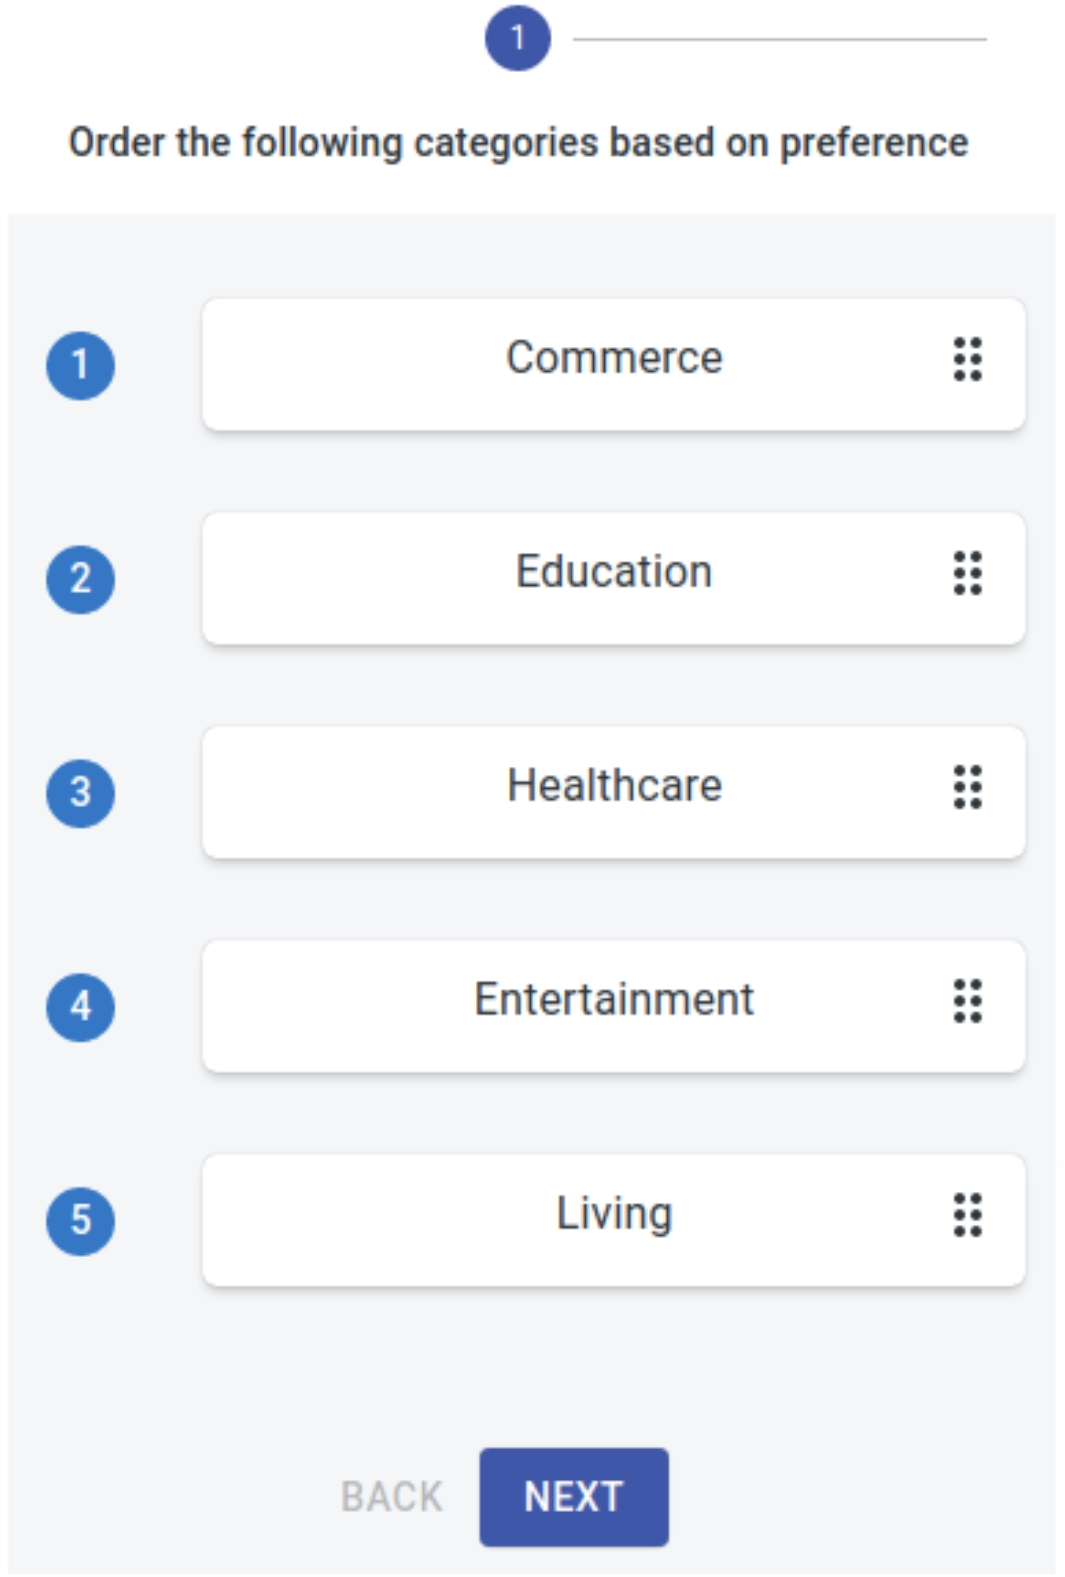
\includegraphics[width=0.85\textwidth]{Chapters/img/backend/ui_stepper_1.png}
        \caption{\centering}
        \label{fig:ui-stepper-1}
    \end{subfigure}
    \hfill
    \begin{subfigure}[b]{0.3\textwidth}
        \centering
        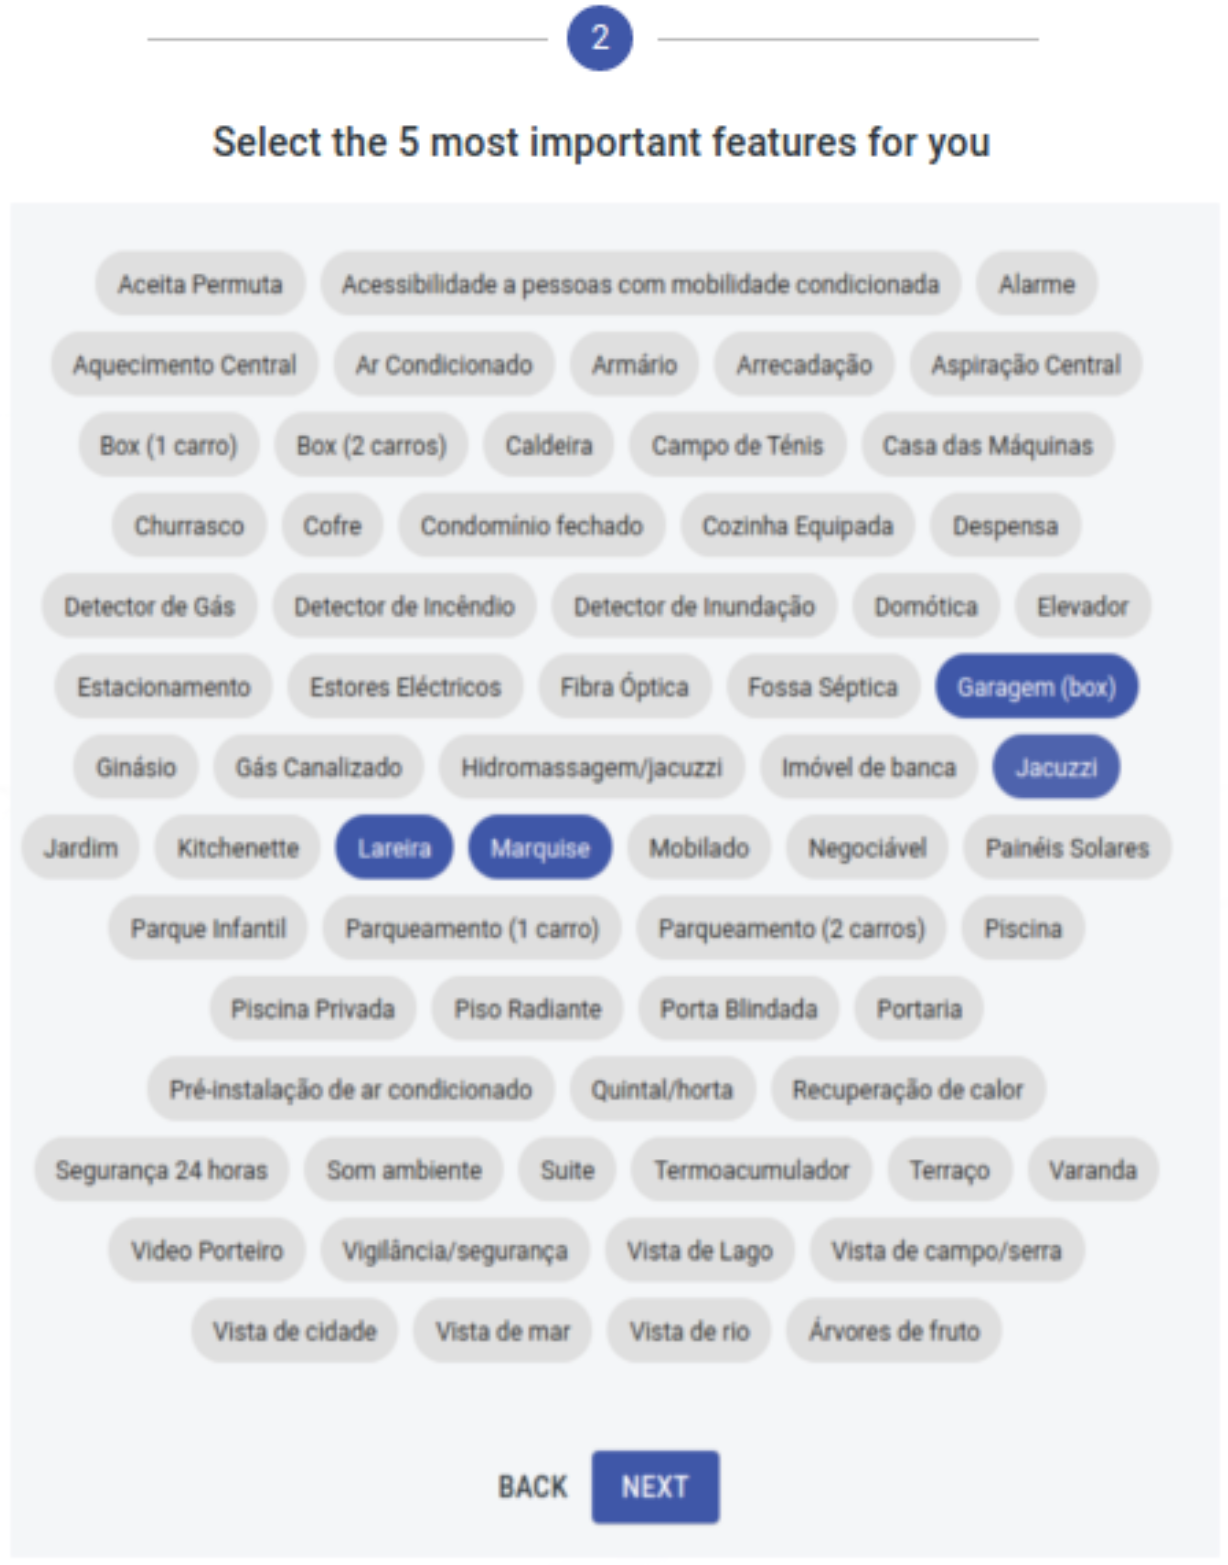
\includegraphics[width=0.99\textwidth]{Chapters/img/backend/ui_stepper_2.png}
        \caption{\centering}
        \label{fig:ui-stepper-2}
    \end{subfigure}
    \hfill
    \begin{subfigure}[b]{0.3\textwidth}
        \centering
        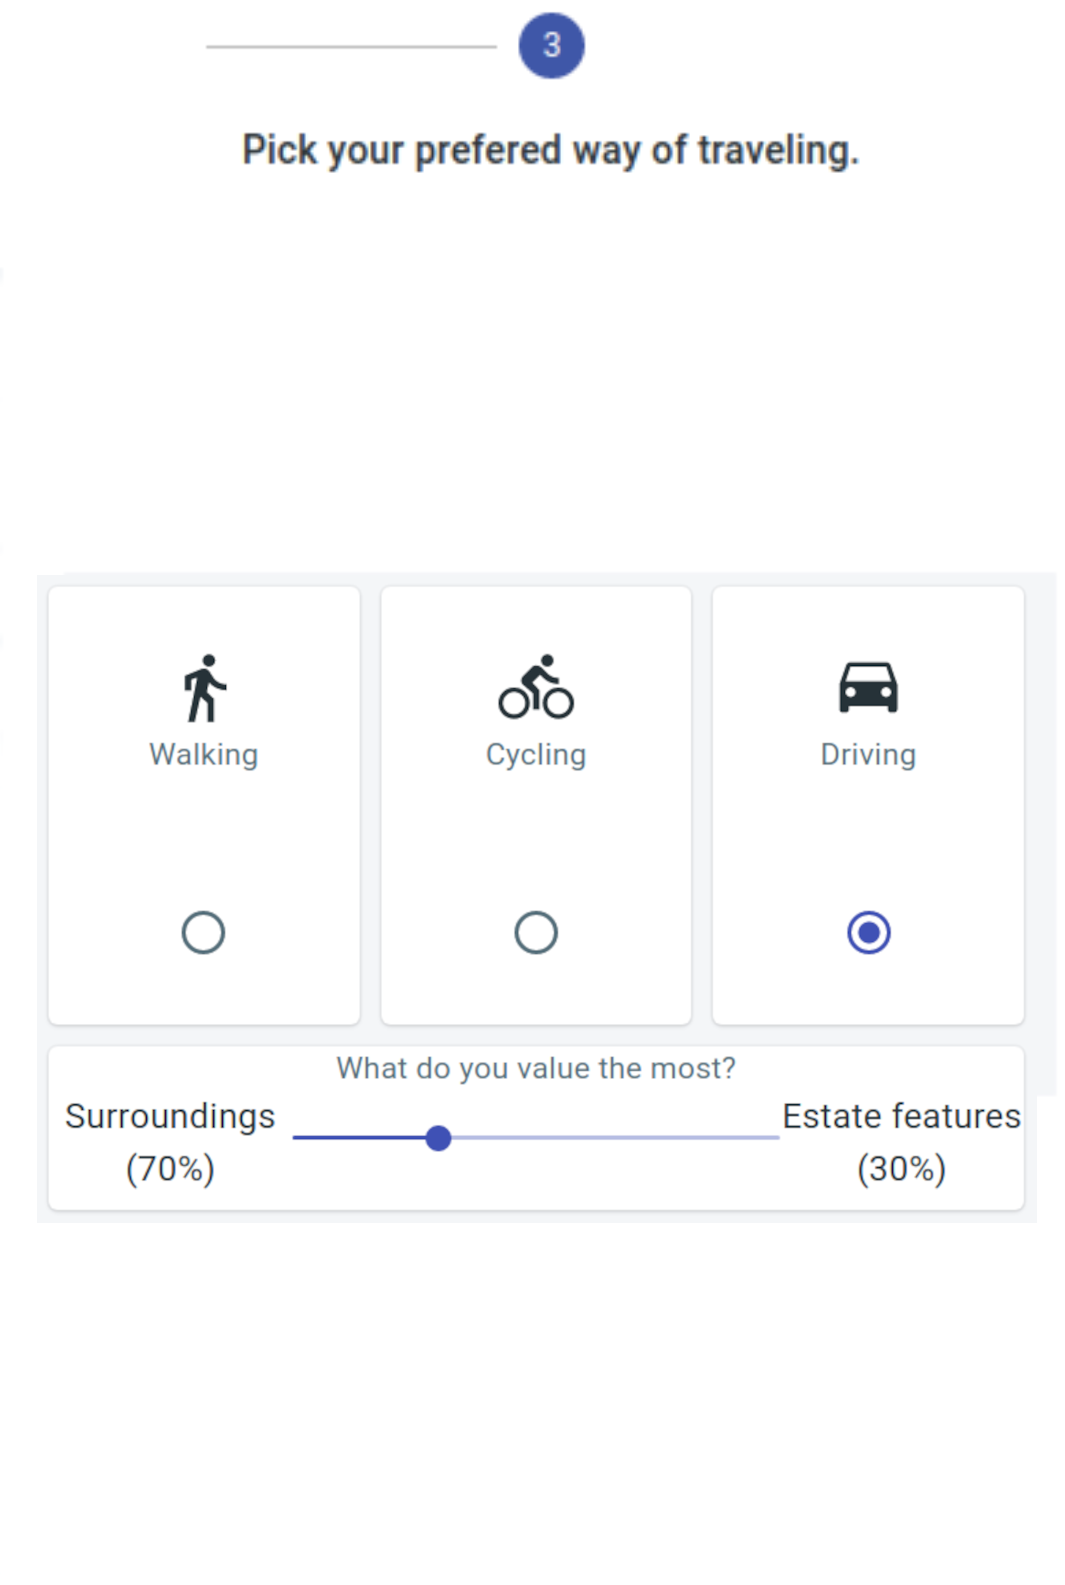
\includegraphics[width=0.85\textwidth]{Chapters/img/backend/ui_stepper_3.png}
        \caption{\centering}
        \label{fig:ui-stepper-3}
    \end{subfigure}
    \caption{Profile creation steps}
    \label{fig:profile-stepper}
\end{figure}

As the authentication credentials were already stored in \acrshort{aws} we have decided to also use another one of their services to store the remainder of user information, which led to the decision of picking DynamoDB a hosted NoSQL database as a storage solution.

\begin{lstlisting}[float, language=Java, caption={[User data model for DynamoDB]{Data model of the User in DynamoDB}}, captionpos=t]
"User": {
    "id": "String",
    "username": "String",
    "ServicePreferences": "List",
    "FeaturePreferences": "Number Set",
    "travelMode": "String"
}
\end{lstlisting}

Personal information was stored according to model shown in Fig. \ref{fig:dynamo-model}, composed of the following elements: 

\begin{enumerate}
    \item An entry identifier of type string, that also acts as a partition key;
    \item An username that ties the information together with Cognito, acting as a foreign key;
    \item the services preferences, stored inside a list that ensures ordering is maintained;
    \item the feature preferences stored in a number set, composed of the identifiers used in the estates database obtain through scraping;
    \item finally, travel mode a string which identifies the preferred travelling mode;
\end{enumerate}

Just like Cognito, the connection to DynamoDB was done through the available AWS SDK for Java, which allowed the creation and management of the database through code. Data access was done with the help of the \textbf{Spring Data}~\footnote{\url{https://spring.io/projects/spring-data}} project, which facilitates application access to data through the use of repositories, which are created with dynamic query derivation from their names (e.g., for SQL with the following java method declaration: Estate findByID(String idx) is transformed into "SELECT * FROM estates WHERE id = idx", with the data from the query being translated with an \acrshort{orm} based on models previously created to mimic the real tables).

\begin{table}[t]
\centering
\caption[User service endpoints]{API endpoints available to manage user information (/v1/account)}
\begin{tabular}{c|c|c}
Type                     & Endpoint & Description \\ \hline
GET                      & /user    & Retrieve    \\
POST                     & /user    & Create      \\
\multicolumn{1}{l|}{PUT} & /user    & Update     
\end{tabular}

\label{tbl:accountAPI}
\end{table}


\subsubsection{Estate}
\label{sss:estate}

Up until now each service described had their own database, however the \textit{Estate} service shares their data store with the scraping pipeline, pipeline which we will call \textit{Data Gathering Service} (DGS). One of the "microservice rules" is that each service should have their own database service, to allow the decouplement of services. However, in this scenario this was the best option to avoid completely duplicating data without proper purpose and to split the responsibilities of the DGS. This way, DGS is responsible solely for scraping and processing data, while the Estate service is used to interact with other services and with the frontend. And, as the DGS is completely controlled by us, we can schedule the scrapping jobs on time slots which do not interfere with the \textit{Estate} service functioning.

This service ends up being the most 

\begin{enumerate}
    \item Generic data about the location such as the location type, average price, etc...
    \item Map which includes the coordinates retrieved for each estate in the queried location and the representation, in this case of the selected parish;
    \item Some information about the estates in the area, such as most common features and estate distribution by number of bedrooms;
    \item A table with details of all the estates retrieved for the select zone.
\end{enumerate}

Besides the support for the multiple microservices with gRPC and Kafka, it also has a public facing API with the  endpoints describe in Table \ref{tbl:locationEndpoints}.

\begin{table}[h]
\centering
\caption{Endpoints available under /v1/location}
\begin{tabular}{c|c|c}
\textbf{Type}            & \textbf{Endpoint}                   & \textbf{Description}                      \\ \hline
GET                      & /\{type\}/\{location\_id\}/geometry & GeoJSON representing the selected zone    \\
GET                      & /\{type\}/\{location\_id\}/estates  & List of estates inside a zone             \\
\multicolumn{1}{l|}{GET} & /estates                            & Retrieve multiple estates by Id           \\
GET                      & /estate/\{id\}                      & Retrieve an estate                        \\
GET                      & /estate/\{id\}/price\_history       & Obtain price history of a specific estate \\
GET                      & /estate/\{idEstate\}/location       & Obtain location of a specific estate     
\end{tabular}

\label{tbl:locationEndpoints}
\end{table}

\begin{figure}[!t]
    \centering
    \begin{tikzpicture}
        \node{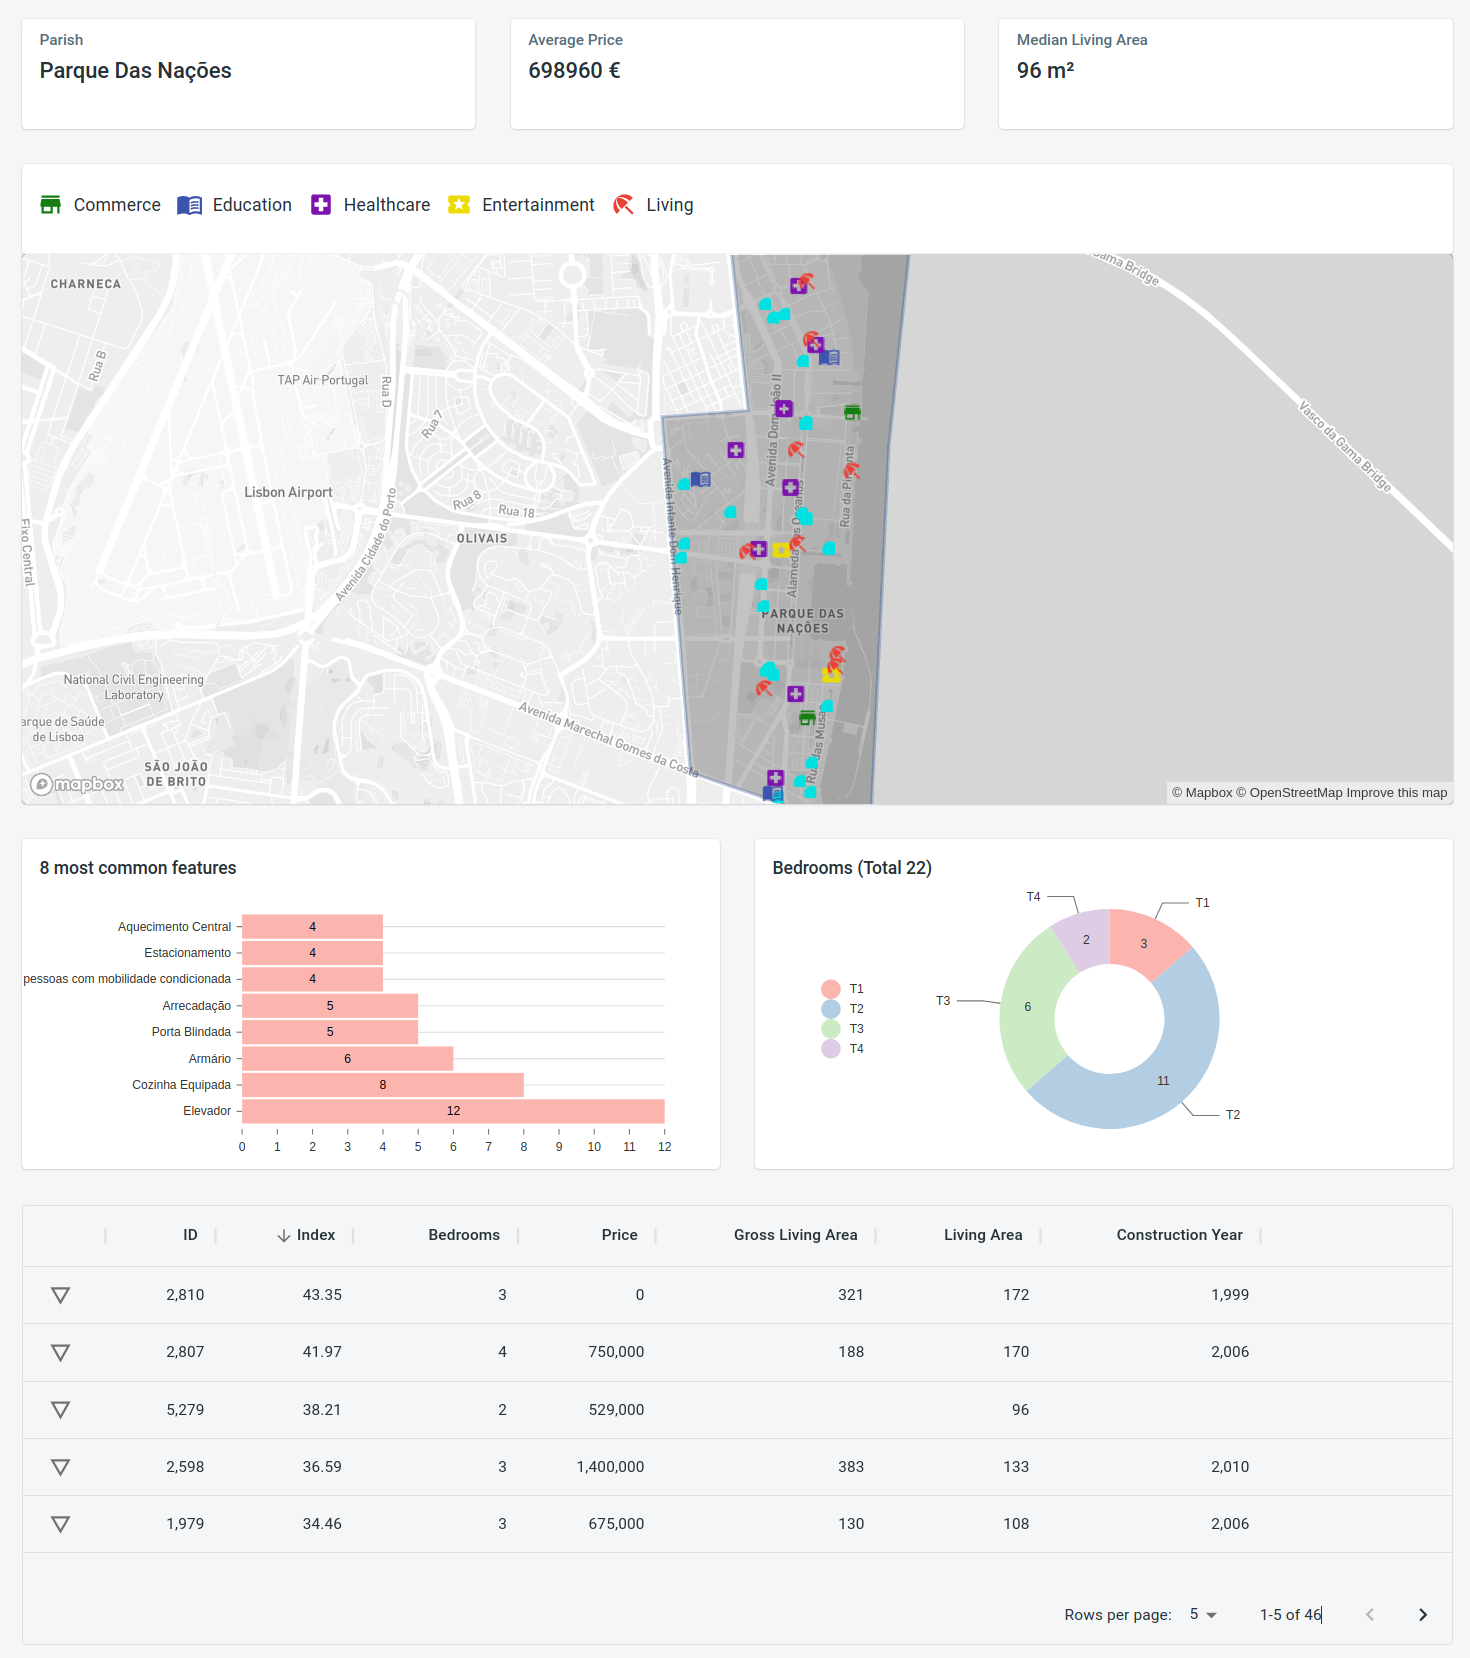
\includegraphics[width=1\textwidth,clip]{Chapters/img/frontend/Overview.png}};
        \node[xshift=-8cm, yshift= 8cm, fill=white, circle, draw=gray]{1)};
        \node[xshift=-8cm, yshift= 4cm, fill=white, circle, draw=gray]{2)};
        \node[xshift=-8cm, yshift=-2cm, fill=white, circle, draw=gray]{3)};
        \node[xshift=-8cm, yshift=-6cm, fill=white, circle, draw=gray]{4)};
    \end{tikzpicture}
    \caption{Overview of the dashboard} 
    \label{fig:overviewDashboard}
\end{figure}

As most of the data in the system relies is geographical, most of the queries are also within the same domain, endpoints like '/parish/1/estates' rely in PostGIS SQL functions like ST\_Contains to intersect estate Point coordinates with zone Polygons. One example of this queries can be seen in listing \ref{lst:geoQueryEstates}.

\begin{lstlisting}[float, language=SQL, label={lst:geoQueryEstates}, caption={[Example of geographical sql query returning a GeoJSON]{Example of a geographical query used in the project that returns the results formatted into a GeoJSON}}, captionpos=t]
SELECT jsonb_build_object('type', 'FeatureCollection', 'features', jsonb_agg(features.feature)) 
FROM ( 
    SELECT jsonb_build_object('type', 'Feature', 'id', id_estate, 'geometry', ST_AsGeoJSON(coordinates)::jsonb, 'properties', to_jsonb(inputs) - 'id_estate' - 'coordinates') AS feature
	FROM (
	    SELECT DISTINCT 
            estate.id_estate, location.coordinates, estate.typology, estate.living_area, estate.gross_living_area, construction_year,
            (SELECT price_history.value FROM price_history WHERE price_history.id_estate = location.id_estate ORDER BY update_date DESC LIMIT 1),
            (SELECT jsonb_agg(id_feature) FROM estate_features WHERE estate_features.id_estate = estate.id_estate) as features
        FROM locationType 
        INNER JOIN location ON ST_Contains(ST_SimplifyPreserveTopology(locationType.shape, SIMPLIFY_RATIO), location.coordinates)
        INNER JOIN estate ON estate.id_estate = location.id_estate
        INNER JOIN price_history ON estate.id_estate = price_history.id_estate
        WHERE locationType.idByType.get(locationType) = locationId) 
	inputs) 
features;
\end{lstlisting}

Most of the geographical queries created were built to return a GeoJSON, as a way to ensure interoperability between all the services and the frontend. Also, some of them had to be optimized to improve the speed of the queries, which also can be seen in the previous example as the shape of location was transformed with ST\_SimplifyPreserveTopology, which simplifies the geometry by removing some of its vertex while maintaining its original structure. Most of the commonly used geometries were also indexed, to ensure a faster access.

\subsubsection{Parameter}
\label{sss:parameter}

One of the most important factors of 15-minute cities is the essential functions that every citizen must be able to perform within a 15-minute radius. For this reason, an exclusive microservice was dedicated to dealing with services and commodities which take part in each function, and that we call  \acrfull{poi}. As a case-study all of the \acrshort{poi} are located in the Lisbon municipality, obtained through Lisboa Aberta~\footnote{\url{http://lisboaaberta.cm-lisboa.pt/index.php/pt/}}, the open Lisbon open data platform. For each function, the following data was gathered:

\begin{itemize}
    \item \textbf{Home} -- another word for estate, it has a dedicated service detail in section \ref{sss:estate};
    %\item \textbf{Work} -- As it would be difficult to track every job location, and
    \item \textbf{Commerce} -- Markets~\footnote{\url{https://dados.gov.pt/pt/datasets/mercados/}};
    \item \textbf{Health care} -- Pharmacies~\footnote{\url{http://dados.cm-lisboa.pt/dataset/farmacias-e-parafarmacias}} and public hospitals~\footnote{\url{http://dados.cm-lisboa.pt/dataset/hospitais-publicos}};
    \item \textbf{Education} -- First cycle (years 1st-4th)~\footnote{\url{https://dados.gov.pt/en/datasets/escolas-publicas-1-ciclo/}}
    \item \textbf{Entertainment} -- Museums~\footnote{\url{https://geodados-cml.hub.arcgis.com/datasets/museus}} and Cinemas~\footnote{\url{https://geodados-cml.hub.arcgis.com/datasets/CML::cinemas/}}.
    \item \textbf{Living} -- Green spaces~\footnote{\url{https://geodados-cml.hub.arcgis.com/datasets/e65d5898bfb443c9b19df421d8341734_0/explore?location=38.743700\%2C-9.155562\%2C13.38}}
\end{itemize}

The \textit{working} social function, mentioned previously during the introduction of the concept, was excluded from our interpretation, as it would exclude most estates searches (e.g., most people cannot afford to live near their workplace) while also saving the trouble of dealing with extra personal information that the user may be hesitant to give.

Each \acrshort{poi} is identified by a category (e.g., Health care and Entertainment), a service (e.g., Hospitals and Museums), a location represented through coordinates and finally, optional metadata to enrich the description of each \acrshort{poi}. As the relevant data is structured and fits a predefined schema we chose to pick PostgreSQL as a datastore, with the data model shown in Fig. \ref{fig:ea-params}. The populate the database data is ingested through a Python script which processes every GeoJSON file gathered previously.

\begin{figure}[h]
    \centering
    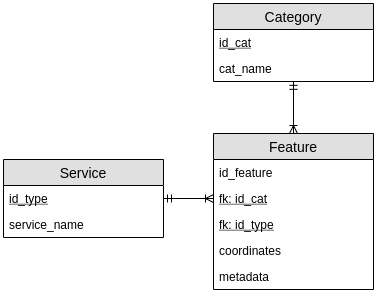
\includegraphics[width=0.5\textwidth,clip]{Chapters/img/backend/ea-params.png} 
    \caption{Parameter data model} 
    \label{fig:ea-params}
\end{figure}

When the user queries the system for a new zone, he is shown in the map where it is located while also being given the option to pick the categories he wishes to see in the map through toggling, as shown in Fig. \ref{fig:overviewMap}. 

\begin{figure}[h]
    \centering
    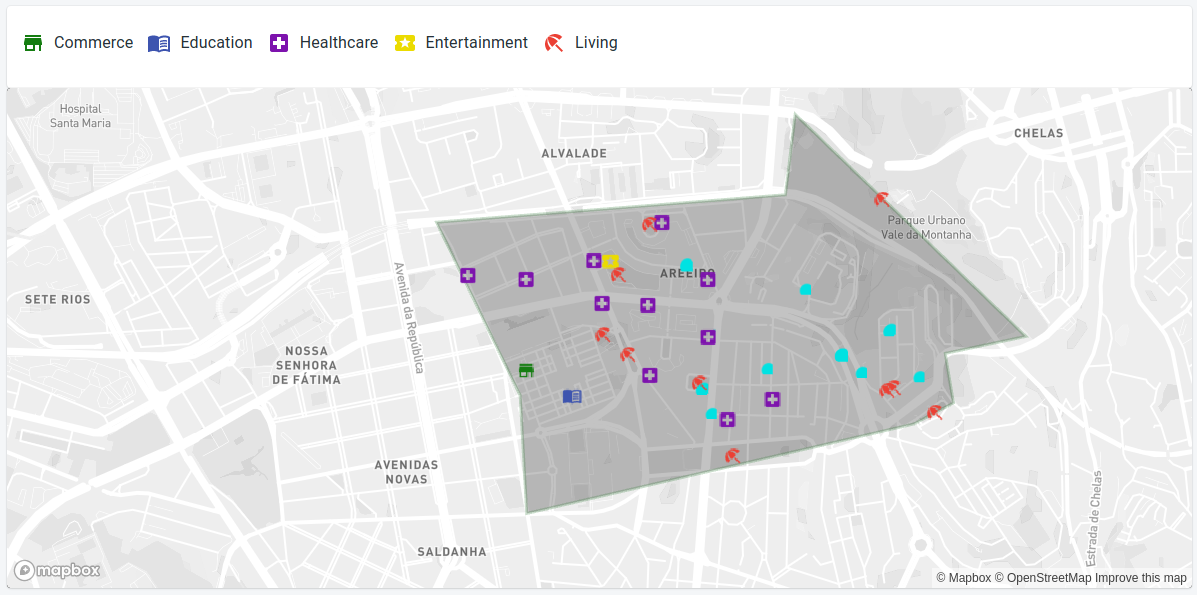
\includegraphics[width=1\textwidth]{Chapters/img/frontend/OverviewMap.png}
    \caption{Map as seen by the user} 
    \label{fig:overviewMap}
\end{figure}

All of this is supported through the following (Table \ref{tbl:paramsAPI}) endpoints available:

\begin{table}[h]
\centering
\begin{tabular}{c|c|c}
Type                     & Endpoint                                             & Description                                                                                                                                                    \\ \hline
GET                      & /features                                            & Retrieve all features with a geometry                                                                                                                          \\
GET                      & /feature/\{id\}                                      & Retrieve feature                                                                                                                                               \\
\multicolumn{1}{l|}{GET} & /category/\{id\}                                     & Retrieve category                                                                                                                                              \\
\multicolumn{1}{l|}{GET} & \multicolumn{1}{l|}{/estate/\{estate\_id\}/features} & \multicolumn{1}{l}{\begin{tabular}[c]{@{}l@{}}Retrieve features within isochrone geometry \\ surrouding the estate (depends on Metrics $\mu$ service)\end{tabular}}
\end{tabular}
\caption{/v1/params endpoints}
\label{tbl:paramsAPI}
\end{table}

\subsubsection{Search}

To facilitate site traversal a text-based search function was implemented with Elasticsearch. Through a search bar, the user is prompted to write the name of a location he wishes to look for, which can be any of the following types: parishes, municipalities, districts, and NUTS (1, 2 and 3). 

\begin{figure}[h]
    \centering
    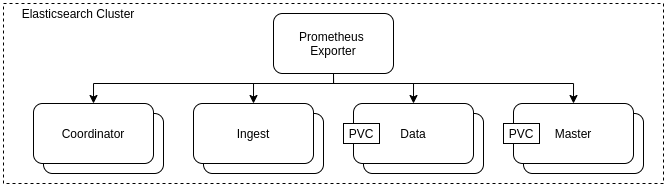
\includegraphics[width=1\textwidth]{Chapters/img/backend/es-architecture-sem-kibana.png}
    \caption{Elasticsearch cluster configuration} 
    \label{fig:es-architecture}
\end{figure}

The Elasticsearch cluster was deployed with the helm chart from Bitnami, and to maintain the goal of the rest of the entire application, it was adjusted to guarantee scalability by splitting the cluster into multiple nodes as seen in Fig. \ref{fig:es-architecture}. As of now, for the current workload, the application was deployed with only an instance of each node. The configuration was also setup to include a \textit{Prometheus exporter} node (details in section \ref{s:monitoring}), which is responsible for collecting metrics from each associated node, but as of now as it was not a top priority to monitor the Elasticsearch cluster, it remains unutilized.

The search functionality relies on location information acquired and used during the scraping phase, as such a Python script was created to ingest the data, but this time in the Elastic Search format, as shown in the following listing. 

\begin{lstlisting}[float, language=Python, caption={[Python data ingestion into Elastic Search]{Snippet of one the implementations done to insert data into the elastic search cluster with Python}}, captionpos=t]
def processDistrict(self, filepath, separator):
    # Colunas: 'Geo Point', 'Geo Shape', 'Dicofre', 'Distrito'
    # TIPOS:    String    ,  GeoJSON   ,  Int     ,  String

    df = pd.read_csv(filepath, sep=separator)

    actions = []
    for index, row in df.iterrows():
        action = {
            "_index": "locations-district",
            "_source": {
                "dist_district_name": row['Distrito'].title(),
                "dist_district_code": row['Dicofre'],
                "type": "District"
            }
        }
        actions.append(action)

    self.insertDataBulk(actions)
\end{lstlisting}

%in Python the same data was obtained from the database and inserted into Elasticsearch. 

%As this only occurs once during startup, and on rare occasions consequence of government updates, having a node dedicated to ingestion is a bit overkill, while at the same time facilitating future expansions.

The search bar was exposed to the frontend through a REST API (/v1/search) built in Spring Boot. It is split into five controllers, four of them for specific searches (e.g., /v1/search/district) and the last one, a generic controller used when the user has not specified the type of location he is looking for (/v1/search/location). For the latter, it has an associated \textit{LocationService} which is responsible for aggregating the data from all other services, allowing us to easily return results similar to the ones presented in Fig. \ref{fig:search-bar}.

\begin{figure}[h]
    \centering 
    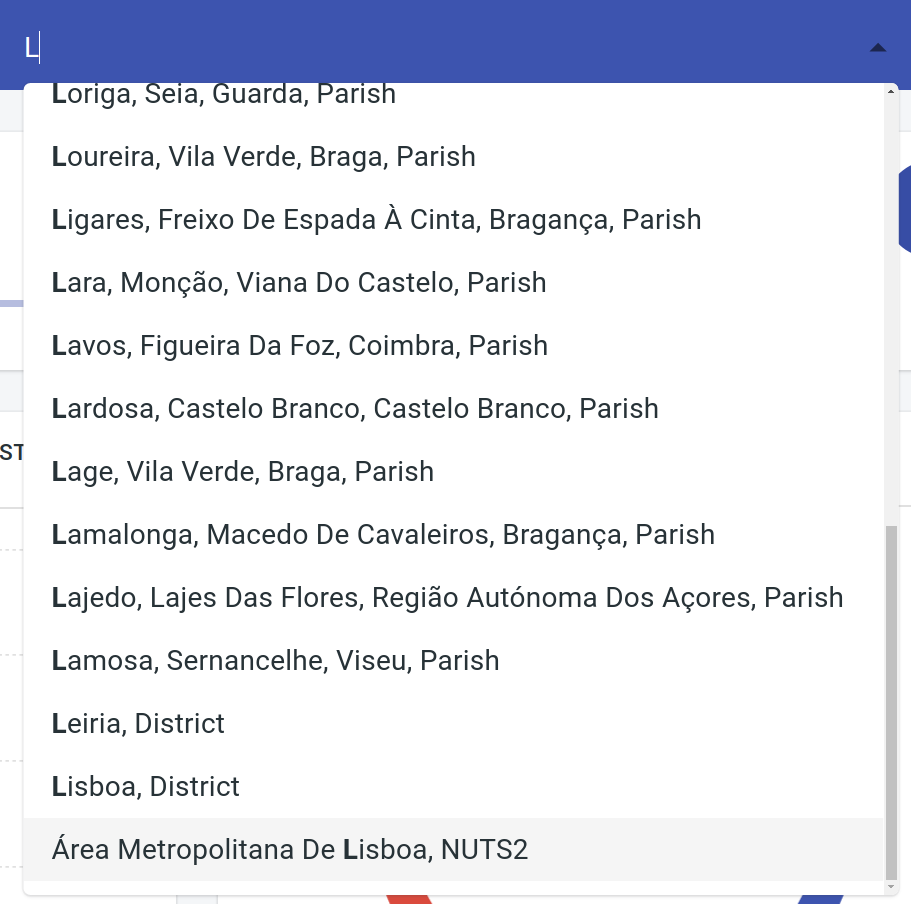
\includegraphics[width=0.4\textwidth]{Chapters/img/backend/search-bar.png}
    \caption{Search bar and results for the letter "L"} 
    \label{fig:search-bar}
\end{figure}

Each service has an associated repository that extends \textit{ElasticSearchRepository} from Spring Data, which works similarly to the repository described in Section \ref{sss:user} and allowed for generic querying of the cluster. However to be able to fine-tune the queries we had to implement a custom repository that each repository also extends, which uses the Elasticsearch full query \acrfull{dsl}. With this we were able to use existing queries such as: \textbf{Match phrase prefix query} which returns documents that contain the words of a provided text, in the same order as provided, with the last term being treated as a prefix, matching any words that begin with that term (e.g., "quick brown f" would match "quick brown fox" and "two quick brown ferrets" but not "the fox is quick and brown"); we also experimented with fuzzy queries, which return documents that contain terms similar to the search term (e.g, box--fox, black--lack, sic--sick, act--cat) but the results became inconsistent with more than two words, as fuzzy queries are term level queries Elasticsearch tries to search for entire phrases in lists of terms, which yields no results (e.g., "casal de cambra" would not find any match with the terms "casal", "de", "cambra" as there is no entry in the index for the whole phrase). 

\begin{figure}[h]
    \centering 
    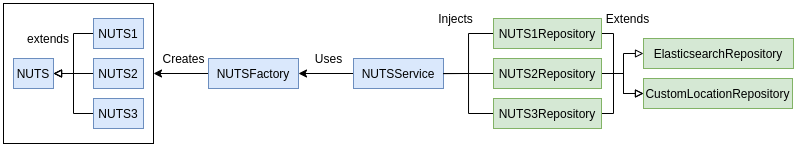
\includegraphics[width=1\textwidth]{Chapters/img/backend/nuts-es-horizontal.png}
    \caption{NUTS Factory pattern} 
    \label{fig:nuts-factory-pattern}
\end{figure}

\acrshort{nuts} are split into three different types, and to avoid creating three different services for each one, we decided to utilize the factory design pattern, as shown in Fig. \ref{fig:nuts-factory-pattern}. The \textit{NUTSService} now interacts solely with the NUTSFactory, and all its functions have a return type of the parent, NUTS. However, when fetching NUTS through the custom repository created and mentioned previously, Elasticsearch \acrshort{api} returns the results as \textit{SearchHits} instead of mapping them to the corresponding data models. To overcome this, we used reflection to determine the type of the instance and created the appropriate object, as seen in listing \ref{lst:nuts-reflection-snippet}. \\

\begin{lstlisting}[float, language = Java, caption={NUTS reflection snippet}, label={lst:nuts-reflection-snippet}, captionpos=t]
    String className = "microservice.search.model."+nutsType.getNutsType();
    Class[] cArg = {String.class,String.class, String.class, String.class};

    NUTS nut = (NUTS)Class
            .forName(className)
            .getDeclaredConstructor(cArg)
            .newInstance(id,regionName,regionCode,nutsType.getNutsType());
\end{lstlisting}

During the mapping of objects to their respective counterparts in the Elasticsearch cluster, text analysis had to be configured, which is the process of converting unstructured text, like the text fields in each object, into a structured format that's optimized for search. This configuration is done via a \acrshort{json} file and may be composed of three building blocks: character filters, tokenizers, and token filters.

\begin{itemize}
    \item \textbf{Character filters} receive the original text as a stream of characters and can transform the stream by adding, removing, or changing characters (e.g., converting hindu-arabic numerals to their arabic-latin equivalents).
    \item \textbf{Tokenizer} receives a stream of characters, breaks it up into individual tokens (words), and outputs a stream of tokens. For instance, a \textit{whitespace} tokenizer breaks text into tokens whenever it uses any whitespace. It is also responsible for recording the order or position of each term and the start and end character offsets of the original word which the term represents. An analyzer must always have one tokenizer. For our application, we chose the \textbf{edge\_ngram} tokenizer, a common tool for \textit{search-as-you-type} queries, which first breaks text down into words whenever it encounters one of a list of specified characters, then it emits \textit{\gls{n-gram}s} of each word where the start of the N-gram is anchored to the beginning of the word.  
    \item \textbf{Token filter} receives the token stream and may add, remove, or change tokens. For example, in our case it was configured to use the following filters: \textbf{lowercase} token filter converts all tokens to lowercase and \textbf{ASCII folding}, which converts alphabetic, numeric, and symbolic characters that are not in the Basic Latin Unicode block (first 127 characters) to their ASCII equivalent, if it exists (e.g., changing é to e).
\end{itemize}

The following endpoints (Table \ref{tbl:searchAPI}) are made available to the public, where \$type is used to simplify the table, in the code there's an endpoint for each of these scenarios for the multiple types of locations: NUTS, districts, municipalities, and parishes. 

\begin{table}[h]
\centering
\caption[Endpoints available in the search API]{Endpoints available in the search microservice at /v1/search.}
\begin{tabular}{c|c|c}
Type                     & Endpoint                                                & Description                                 \\ \hline
GET                      & /\$type (ex: /municipalities)                           & Retrieve all                                \\
GET                      & /\$type/\{name:\textasciicircum{}{[}A-zÀ-ú{]}\{1,27\}\} & Retrieve by name, validated through regex   \\
\multicolumn{1}{l|}{GET} & /\$type/\{code\}                                        & Retrieve by code                            \\
\multicolumn{1}{l|}{GET} & /locations                                              & Searchs all types at the same time, by name
\end{tabular}

\label{tbl:searchAPI}
\end{table}


\subsubsection{Metrics}
\label{sss:metrics}


To enrich the user experience, and truly bring to life the 15 minute concept, it was important to display relevant information about each zone pertaining the containing estates. The metrics microservice requires information scattered through out all the services and as such, it required an efficient way to communicate. 

The metrics that depend solely on estates (Median price, median square metre, most common features and typology distribution) are all requested simultaneously to the estate service through Kafka. The information is request synchronously, something Kafka is not usually associated with. To achieve the request-reply pattern, a correlation ID is associated with each record, allowing Kafka to identify each transaction and correlate requests/replies. As of version 2.1.3, Spring Kafka added support for the Request Reply pattern out-of-the-box which abstracts some of the previous concepts.

\begin{figure}[h]
    \centering 
    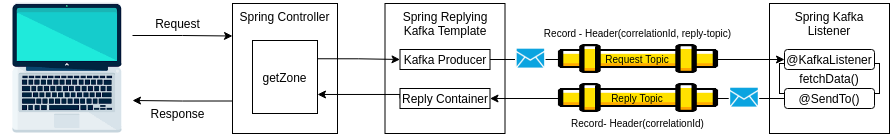
\includegraphics[width=1\textwidth]{Chapters/img/backend/KafkaReqReply.png}
    \caption{Synchronous Request-Reply with Apache Kafka} 
    \label{fig:ReqRepKafka}
\end{figure}

As seen in Fig. \ref{fig:ReqRepKafka}, the user sends a request to the controller asking for information about the zone. The endpoint utilizes the \textbf{kafka reply template} to create a message which includes all the necessary header information such as the \textit{correlation id}, additional information such as \textit{zone id} and the \textit{reply topic} it expects to hear a response from, are manually configured. 

In the other microservice, a \textbf{Kafka Listener} was implemented which is actively waiting for messages, the method is also annotated with \textbf{SendTo} to provide a reply message. The object returns by the listener is automatically wrapped into a reply message, the \textit{correlation id}, and the reply is sent to the specified \textit{reply topic}, which eventually is return to the user.

Since estate data is scrapped and stored every 7 days, there always the guarantee that whatever was fetched up to that day is guaranteed fresh as such, to avoid wasting time and resources of having to constantly communicate with other microservices, data is stored in a MongoDB node associated with this microservice. In every request to \textbf{getZone} (Fig. \ref{fig:ReqRepKafka}), we verify if the data is fresh based on the date it was gathered, and if it is, we can simply query the database and answer the request instantly.


%% ===================================================== Index =============================================================================
\paragraph{Index} is used to rate an estate according to the users social and real estate preferences. To calculate this rating, a weight was associated with each choice. 

As the concept accounts for five main social functions, each had an associated weight that started at 30 and would decrease in steps of 5 (e.g., 30, 25, 20, 15, and 10), associating 30 with the users first option and 10 with the last. Associated to each social function, there are multiple services, which at the moment are averaged down and considered as one, but can easily in the future be altered to account for each specific service. The previous idea can be translated into the following equation:

\begin{equation}
    SocialIndex = \sum_{sf = social\_function} sf \ weight(\%) * max(1, Avg(\frac{ideal\_distance }{dist<estate,service>})
\end{equation}

The ideal distance was considered based on the idea that within a 5 minute window everything is still close enough. As the distance varies according to the chosen travel mode, three values were chosen for each of them, as depicted in Table \ref{tbl:idealTravelDistance}.

\begin{table}[h]
\centering
\caption{[Ideal travel distance in the 15-Minute City per travel mode]{Our idealized travel distance values. Within this range, it is considered that it is not an annoyance to travel somewhere}}
\begin{tabular}{c|c}
Travel Mode & Distance (m) \\ \hline
walking     & 400          \\
cycling     & 1300         \\
driving     & 3000        
\end{tabular}

\label{tbl:idealTravelDistance}
\end{table}


For estate features, since the user can select between 1 and 5 options, the weights are calculated based on the number of options (e.g., $\frac{number \ of \ features}{features \ weight \ \%}$ ), so the feature index arises from the following formula

\begin{equation}
    FeatureIndex = \frac{features \ weight \ \%}{\#user\_selected\_features} * \#relevant\_features
\end{equation}

Both sections are then combined to create the \textbf{index} that always yields results between 0 and 100\%:

\begin{equation}
    Index = (SocialIndex * SocialWeight) + FeatureIndex
\end{equation}

As mentioned previously, and as seen through the equation, to calculate the index, it requires information from multiple points of the system and even external APIs:

\begin{itemize}
    \item \textbf{User} information such as favorite features, social preferences, travel mode;
    \item \textbf{Location} retrieving the GeoJSON from the selected zone;
    \item \textbf{Estates} obtain a list of estates from the selected zone;
    \item \textbf{Parameters} list of points of interest surrounding the estates;
    \item \textbf{Isochrone} map depicts the area accessible from a point within a certain time treshold, information which was gathered from the Mapbox API \footnote{\url{https://docs.mapbox.com/api/navigation/isochrone/}}.
\end{itemize}

Fig. \ref{fig:IndexSequenceDiagram} shows the sequence of actions made to calculate the index, the main idea is that when a user requests a new zone, all the estates in that specific area are fetched, if they already have an associated isochrone for the specified travel model it is used to calculate the index, otherwise a request is made to the mapbox \acrshort{api} to calculate it and store it.

\begin{figure}[h]
    \centering 
    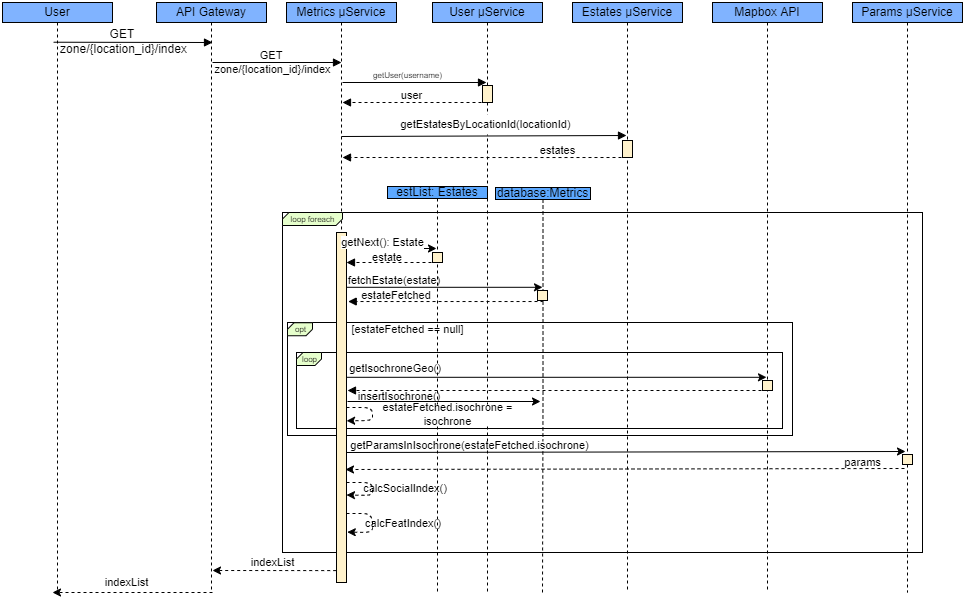
\includegraphics[width=1\textwidth]{Chapters/img/backend/SequenceDiagram.png}
    \caption{Index calculation sequence diagram} 
    \label{fig:IndexSequenceDiagram}
\end{figure}

Unlike the previous case which used Kafka as an intermediary to communicate between services, the index calculation only uses \textbf{gRPC} to interact with all the services. For this interaction a stub was defined for each microservices in the client side (metrics microservice) and a gRPC server in the respective microservices. To communicate a \textit{.proto} file had to be created, to define the services and messages required to communicate. A particularity of this definition its that User is composed by two submessages, similar to OOP concepts, where in this case \textit{features} and \textit{services} have their own definitions to mimic lists.

\begin{lstlisting}[float, language=Java, caption={[GRPC message and service definitions]{GRPC message and service definitions for communication}}, captionpos=t]
syntax = "proto3";
option java_multiple_files = true;
package demo.interfaces.grpc;

message User{
  message ListFeatures{
    repeated int32 feature = 1;
  }

  message ListServices{
    repeated int32 services = 1;
  }

  string id = 1;
  string username = 2;
  ListFeatures features = 3;
  ListServices services = 4;
  int32 surroundingsPercentagePreference = 5;
  int32 estateFeaturesPercentagePreference = 6;
  string travelModel = 7;
}

message Username{
  string username = 1;
}

service UserService {
  rpc getUserByUsername(Username) returns (User);
}
\end{lstlisting}

To obtain the corresponding data access classes and services, the proto file had to be compiled, isntead of doing it manually the process was automatized with Maven and \textit{Maven Protocol Buffers Plugin}~\footnote{\url{https://www.xolstice.org/protobuf-maven-plugin/}}. After the compiler creates the \textit{.java} files for each message type and service, it is now possible to implement the client and server stubs, which can be seen in the following listings.

\begin{lstlisting}[float, language=Java, caption={Java service for GRPC communication}, captionpos=t]
@Service
public class UserServiceImpl{
    @GrpcClient("user-service") 
    private UserServiceBlockingStub userServiceBlockingStub;

    public User getUserByUsername(String username){
        Username request = Username.newBuilder().setUsername(username).build();
        demo.interfaces.grpc.User user;
        try{ user = userServiceBlockingStub.getUserByUsername(request);
        } catch (StatusRuntimeException e){ return null; }
        return new User(user);
    }
}
\end{lstlisting}

The main advantage with gRPC is that there is no need to handle the serialization and deserialization of the transmitted objects, especially when using the same language on both the server and client. When the proto file was compiled the \textbf{UserServiceImplBase} was created, which can be used on the server with an implementation for the defined services, which can then be called by the client as remote procedure calls.

\begin{lstlisting}[float, language=Java, caption={Service definition}, captionpos=t]
@GrpcService
public class UserServiceImpl extends UserServiceGrpc.UserServiceImplBase {
    @Autowired private DynamoService dynamoService;
    @Override 
    public void getUserByUsername(Username request, StreamObserver<User> responseObserver){
        String username = request.getUsername();
        UserDynamo user = dynamoService.getUserByUsername(username);

        ListFeatures.Builder listFeaturesBuilder = ListFeatures
                .newBuilder()
                .addAllFeature(user.getFeaturePreferences()
                                .stream()
                                .map(Integer::parseInt)
                                .collect(Collectors.toList()));

        ListServices.Builder listServicesBuilder = ListServices
                                .newBuilder()
                                .addAllServices(user.getServicePreferences());

        User.Builder userBuilder = User.newBuilder()
                .setId(user.getId())
                .setUsername(user.getUsername())
                .setFeatures(listFeaturesBuilder.build())
                .setServices(listServicesBuilder.build())
                .setSurroundingsPercentagePreference(user.getSurroundingsPercentagePreferences())
                .setEstateFeaturesPercentagePreference(user.getEstateFeaturesPercentagePreferences())
                .setTravelModel(user.getTravelMode());

        responseObserver.onNext(userBuilder.build());
        responseObserver.onCompleted();
    }
}
\end{lstlisting}

The following endpoints (Table \ref{tbl:metricsAPI}) are available to the public.


\begin{table}[h]
\centering
\begin{tabular}{c|c|c}
Type                     & Endpoint                                          & Description                                                                                                              \\ \hline
GET                      & /estate/\{estate\_id\}/isochrone/\{travel\_mode\} & \begin{tabular}[c]{@{}c@{}}Retrieve estate isochrone geometry \\ based on travel mode\end{tabular}                       \\
GET                      & /estate/\{estate\_id\}/params                     & \begin{tabular}[c]{@{}c@{}}Retrieve params inside an estate \\ (uses Params $\mu$service)\end{tabular}                       \\
\multicolumn{1}{l|}{GET} & /zone/\{location\_id\}/index                      & \begin{tabular}[c]{@{}c@{}}Calculates the index for the estates \\ in a zone,  to the user who requested it\end{tabular} \\
\multicolumn{1}{l|}{GET} & /zone/\{location\_id\}                            & \begin{tabular}[c]{@{}c@{}}Retrieves/Calculates metrics \\ for the specific zone\end{tabular}                                                                   
\end{tabular}
\caption{Endpoints available at /v1/metrics}
\label{tbl:metricsAPI}
\end{table}

With access to all of this information, the frontend is capable of presenting to the user the metrics shown in Fig. \ref{fig:overviewMetrics}.

\begin{figure}[h]
    \centering 
    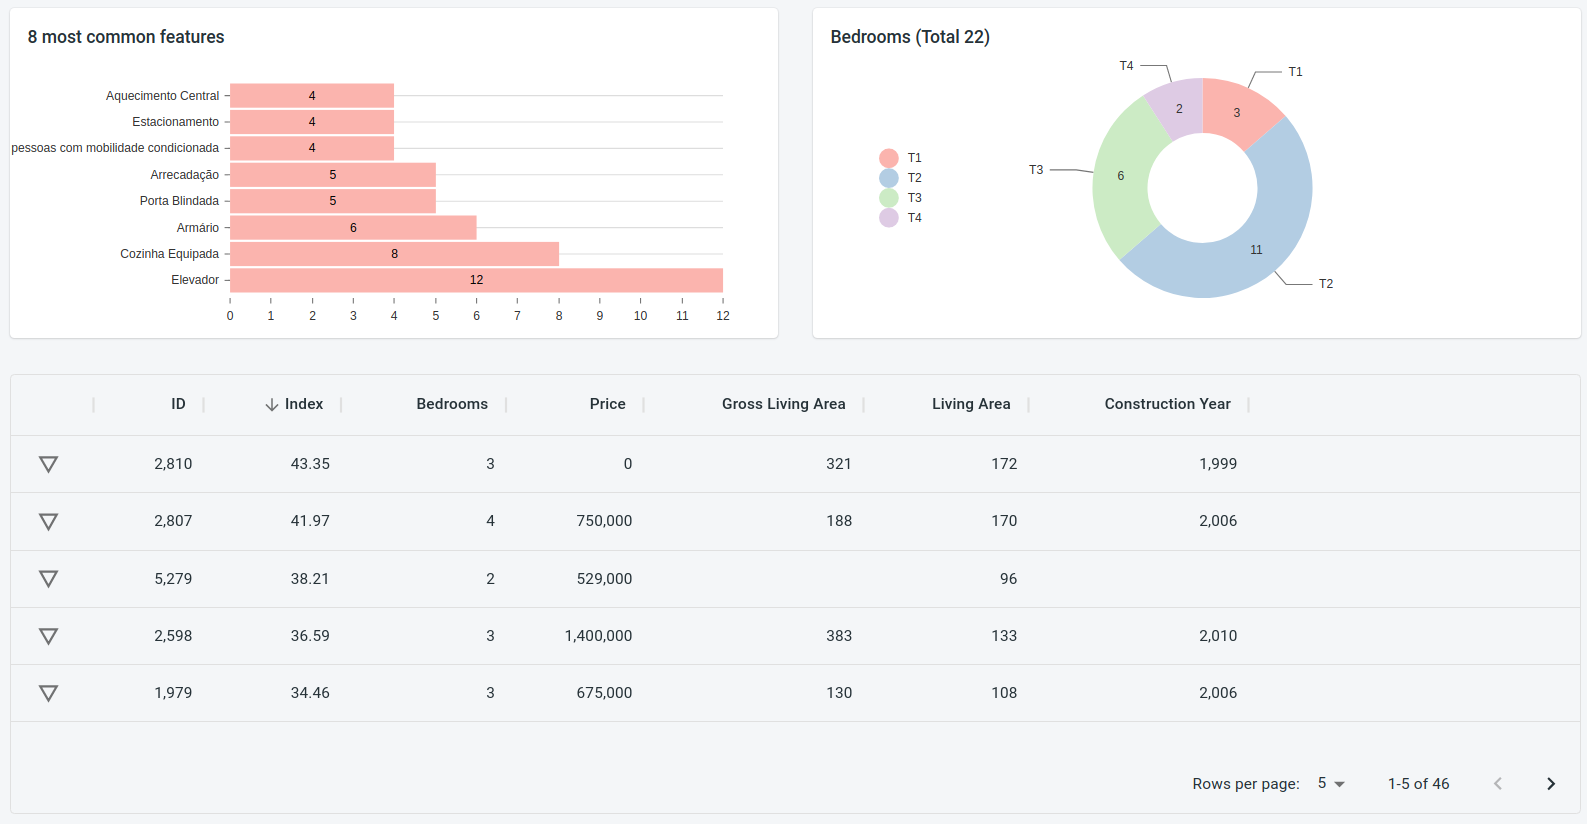
\includegraphics[width=1\textwidth]{Chapters/img/frontend/OverviewMetrics.png}
    \caption{Dashboard - metrics section} 
    \label{fig:overviewMetrics}
\end{figure}





%\section{Index}
%\label{s:index}

%\input{Chapters/implementation/Index}

\section{User Interface}
\label{s:user-interface}
%\chapter{User Interface}
%\label{ch:ui}
 
All the previous work becomes irrelevant without adding a way for the user to interact with the system. This section describes the work that went into the creation of the frontend application to support the 15-Minute city concept.

\subsection{Implementations}
\label{ss:ui-implementations}

Web requirements keep changing, with developers having to support dozens of different browsers, devices, and resolutions. Enter the frontend frameworks, a solution ready to deal with all these problems, on top of it, it also implements multiple functions such as routing, saving development time by not having to reinvent the wheel. In the following sections, we will analyse some of the most popular tools currently available in the market, and how they fare against each other.

\subsubsection{Angular}
\label{sss:angular}

Angular is a component based framework that follows a tree structure, where there is a root with an infinite possibility of children and sibling components. Parents can communicate with children by binding information to them, but a child is unaware of the origin of the data, if it wishes to communicate with the parent, an event has to be emitted. This structure makes components reusable and self-contained.

Components are classes annotated with \textbf{@Component}, and consist of three separate files: .ts, .css and .html. Each component provides a series of life cycle hooks, as seen in the transitions in Fig. \ref{fig:angular-lifecycle}.

\begin{figure}[H]
	\centering
	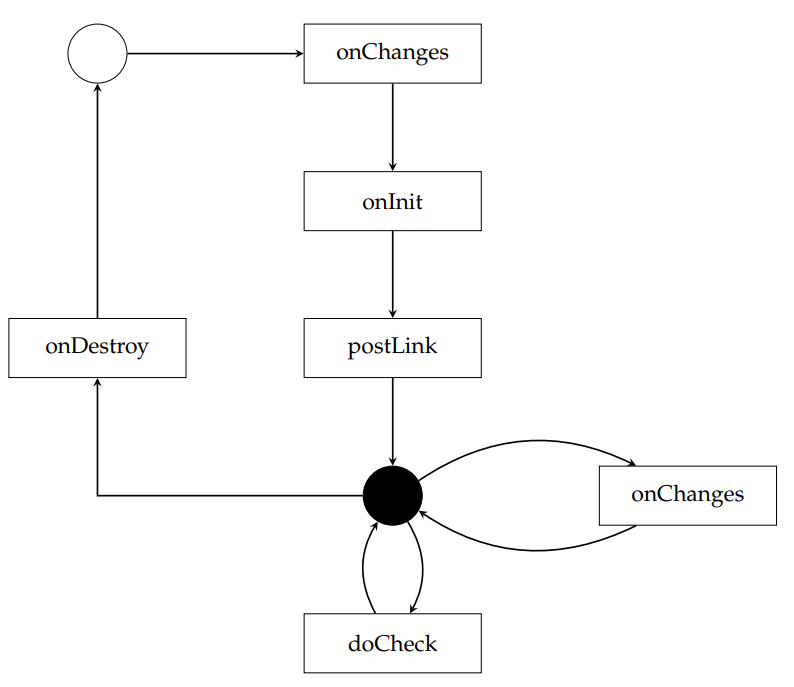
\includegraphics[width=0.75\linewidth]{Chapters/img/frontend/angular-lifecycle.png}
	\caption{Angular life-cycle \cite{react-lifecycle}}
	\label{fig:angular-lifecycle}
\end{figure}

\begin{itemize}
    \item \textbf{onInit} is executed once per component upon creation of the component. It is meant to be used for initial setup and registration of further event handlers.
    \item \textbf{onChanges} is a callback executed whenever a one-way bound variable is updated. It typically occurs during two different stages of the life cycle. Initially, upon creation of the component when initial values for the variables are passed to the component, the method is executed even before the \textit{init} callback. The second time, and which may occur multiple times, is during the lifespan of the component. Whenever a binding is updated, the \textit{onChanges} callback is called with a reference to the variable;
    \item \textbf{doCheck} is called whenever the internal change detection cycle of AngularJS is executed. It provides the possibility to implement custom change detection procedures.
    \item \textbf{onDestroy} called when the component becomes detached from the DOM and the corresponding scope is destroyed
    \item \textbf{postLink} called after the initial setup has been completed and the DOM is constructed. Access to children elements is still restricted, due to asynchronous template loading of child elements in AngularJS.
\end{itemize}

Angular also uses Service, a class with a narrow and well-defined purposed, which angular distinguishes from components to increase modularity and reusability. By separating a component's view-related functionality from other kinds of processing, component classes can remain lean and efficient. A component can delegate certain tasks to services, such as fetching data from the serer, validating user input, etc...  By defining such processing tasks in an injectable service class, it makes those tasks available to any component.

This idea of injecting service classes comes from the concept of \acrfull{di}, a design pattern in which a class requests dependencies from external sources rather than creating them. In Angular, components consume services; that is, a service can be injected into a component, giving the component access to that service class. In angular, services are annotated with \textbf{@Injectable()}.


\subsubsection{React}
\label{sss:react}

\todo[inline]{Decidimos deixar este capitulo para o fim, vamos tentar entender mais tarde se faz sentido manter aqui ou no SotA. A dúvida está em que apesar de ser sobre react, está muito relacionada com padrões de desenho de software.

Possivel solução: mudar nome de react para 'design patterns', elaborar as secções de MVC, MVVM e manter o Flux. Passar as informacoes do react em si, para a implementacao.}


%% -- Created: 07-07-21
%% -- Last edit: 07-07-21

React \footnote{\url{https://reactjs.org/}} is a Javascript library used to build \acrshort{ui}s, it can be used in isolated parts or to create \acrshort{ui}s for whole web applications. React focus entirely on the creation of Views, as such it does not enforce any architecture pattern.

React relies on composition to build complex \acrshort{ui}s from small building blocks called \textbf{components}~\cite{react-lifecycle-functions}. Components consist of a render method that returns a description of what to render, which  can either be HTML or other react components. The description of what to render uses a syntax called \acrlong{jsx} (\acrshort{jsx}) which is a combination of HTML and Javascript. 


React applications have two essential building blocks \textbf{state} and \textbf{props}. State allows components to "remember" things, but it can also be altered based on user interaction or other actions within the application~\cite{react-state-and-lifecycle}. State is not mandatory, and components with it are called stateful components while states without it are called presentation components.

Props, or properties, are immutable data passed onto a component upon construction. This is what makes React components flexible and reusable, as one component can behave and look differently depending on the props passed to it.

In React, data flows downwards through the component tree using props. For a child component to interact with its parent, callback functions are passed as props. In large applications this is not ideal since it can lead to deep trees, which forces data and callback functions to pass through multiple levels. This process is referred to as "\textbf{props-drilling}" and makes the components tightly coupled and less maintainable.

Each component can be defined as a \textbf{class-based} or \textbf{function} component. A class-based component is created by extending the \textit{React.Component}. The state of this type of components is updated using the method \textit{setState()} and read by using \textit{this.state} within the class. Using the setState() method makes the component re-render which is not the case when mutating the state directly. Class-based components include \textbf{life-cycle} methods that can be used to create more complex behaviour.

This life-cycle methods~\cite{react-state-and-lifecycle} are built-in methods called when a state or prop updates, before or after a component has rendered or when a component is destroyed, as shown in Fig. \ref{fig:react-lifecycle}.

\begin{figure}[H]
	\centering
	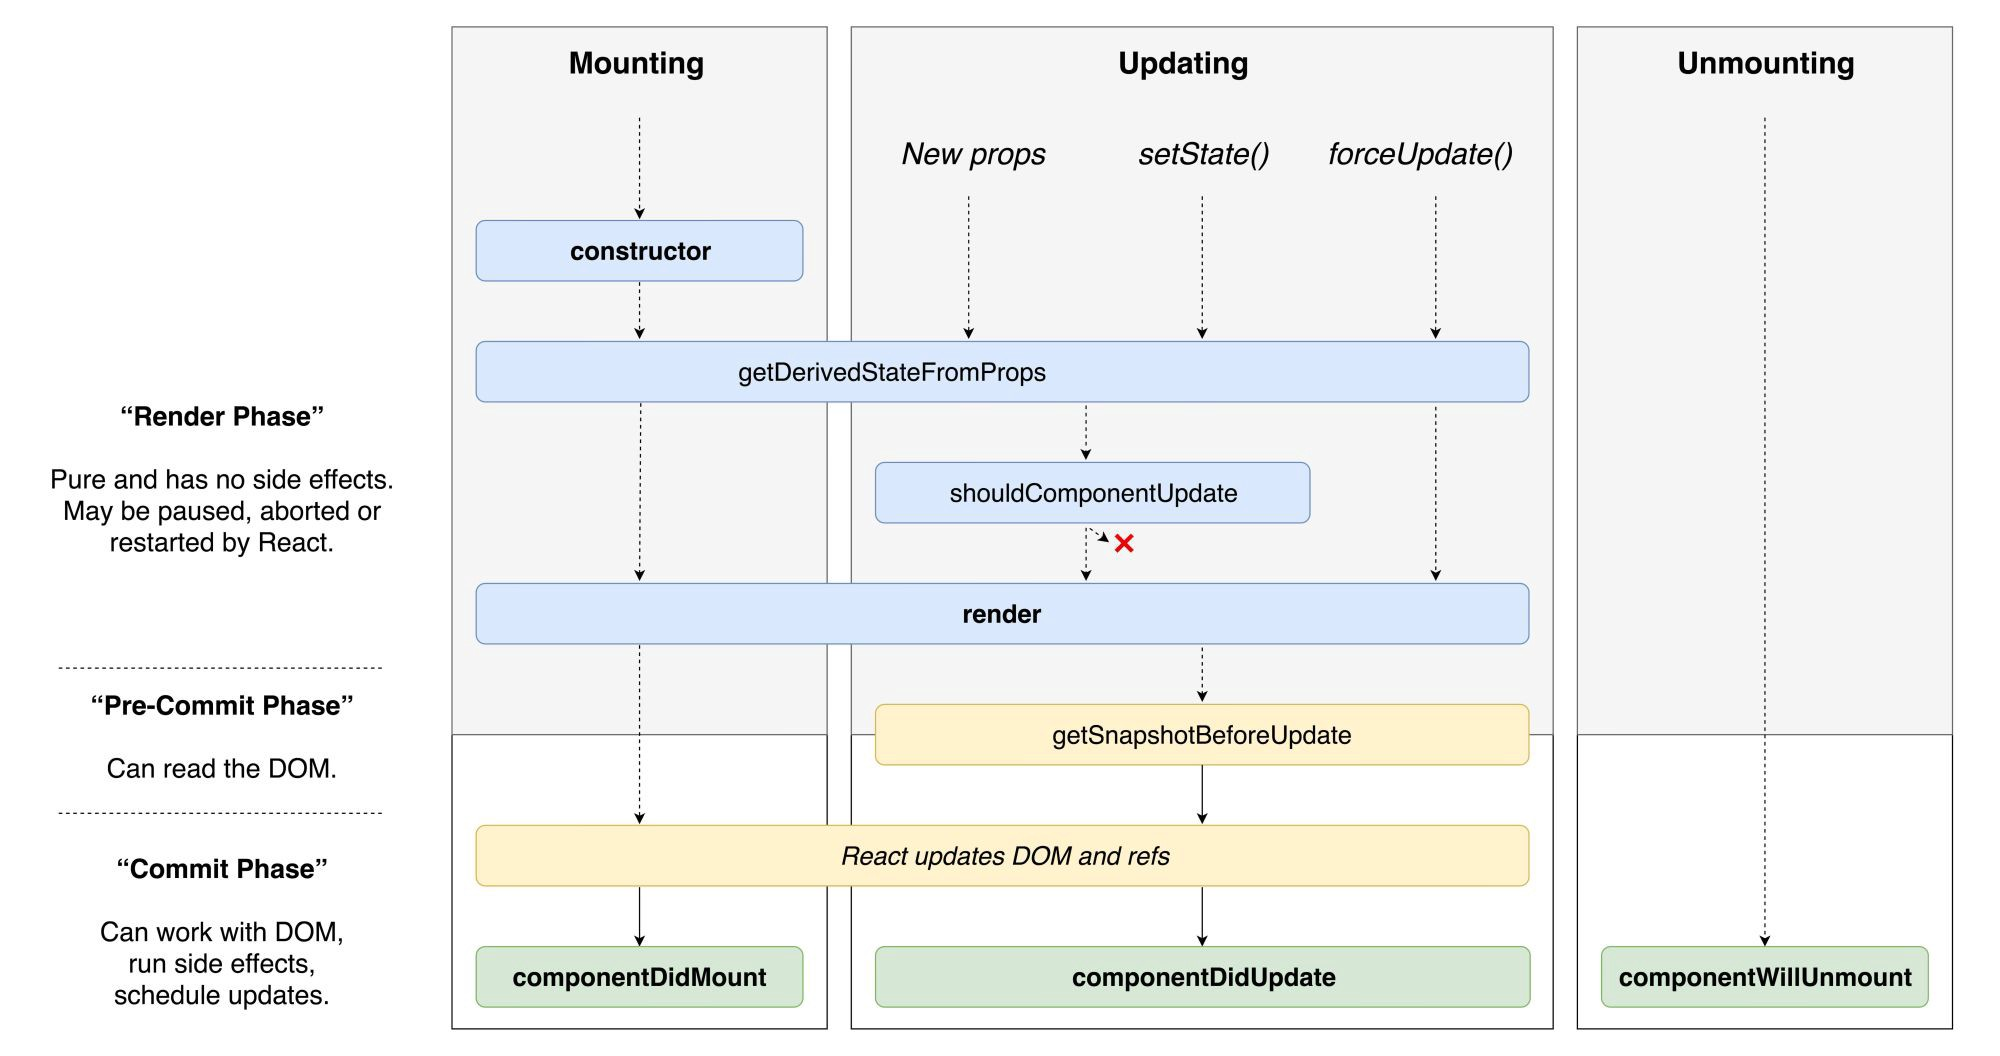
\includegraphics[width=1\linewidth]{Chapters/img/2_background/react-lifecycle.jpeg}
	\caption{React life-cycle \cite{react-lifecycle}}
	\label{fig:react-lifecycle}
\end{figure}

This cycle is split into three phases: \begin{inparaenum}[1)] \item \textbf{mounting}, the birth of the component; \item \textbf{updating}, growth of the component; \item \textbf{unmounting}, the dead of the component \end{inparaenum}. Here's an overview of the most commonly used methods~\cite{react-lifecycle-functions}:

\begin{itemize}
    \item \textbf{render} is the most used. Handles the rendering of components. It is a pure function (no side-effects and always returns the same output with the same inputs) and as such, it should not be used to set the state;
    
    \item \textbf{componentDidMount} is called as soon as the component is mounted and ready. Used to initiate \acrshort{api} calls, if data from a remote endpoint is needed. Updating state here will cause another rendering but it will happen before the browser updates the \acrshort{ui} (to ensure that the user will not see any \acrshort{ui} updates with double rendering).
    
    \item \textbf{componentDidUpdate} happens as soon as the updating happens, its mostly used for updating \acrshort{dom} in response to prop or state changes. State updates here must be done with caution to avoid infinite update loops.
    
    \item \textbf{componentWillUnmount} happens before the component unmounts and is destroyed. Used for data cleanup.
\end{itemize}

Function components are pure functions that accept props as input and return a \acrshort{jsx} element. To given them access to state and life-cycle methods as class-based components, \textbf{React hooks} are used. By combining component functions with hooks, the size and complexity of an application in comparison to class-based components is reduced.

Hooks~\cite{react-hooks} are used for more advanced function components and can also be customized, which promotes re usability of functionality between components. They follow a naming convention starting with the word "use", as can be seen while looking at three of the main hooks:

\begin{itemize}
    \item \textbf{useState} As state does not exists in function components by default, useState is used which preserves the state throughout the lifetime of the component. This hook, and all others, can be used more than once inside the same component;
    \item \textbf{useEffect} allows for the replacement of life-cycle mthods. This hook will execute a function for every rerender of the component by default, but can also be customized to only execute for certain changes;
    \item \textbf{useContext} allows data to be shared between components in the component tree without requiring props-drilling. Data is added to the Context and made available through a \textbf{Provider}.
\end{itemize}

%since State does not exist in a component by default, instead they use a React hook named \textit{\textbf{useState}} which preserves the state throughout the lifetime of the component. This hook, and all others, can be used more than once inside the same component.

%Since life-cycle methods do not exist in function components, they had to be recreated using the \textit{\textbf{useEffect}} hook, which will execute a function for every rerender of the component by default but can be customized to only execute for certain changes.

%Another hook is the \textbf{\textit{useContext}} hook which allows data to be shared between components in the component tree without using props-drilling. Data is added to the Context and made available through a \textbf{Provider}.

The provider takes one property named value where the data for the Context is specified which can be variables, functions, or objects. By wrapping children components inside the Provider component, the Context data can be accessed from any child component using a Consumer available to the Context instance as well. Worth noting that the application is not limited to one context.

\subsection{Flux - Architectural Pattern}
\label{ss:flux}

%% -- Created: 07-07-21
%% -- Last edit: 07-07-21

Since React does not enforce architectural patterns all functionality for a web application could, in theory, be placed in a single module that would handle everything from data fetching to business logic. But that leads to an error-prone application that would be hard to maintain, therefore architectural patterns are necessary to build well-structured high-quality applications.

As React applications have an unidirectional data flow, as described before, each component has its own data stored in its state. For larger React applications, more advanced architectural patterns are needed to make the application maintainable, such as \textbf{Flux} \footnote{\url{https://facebook.github.io/flux/}}.

The flux architectural pattern was invented by Facebook, it was derived from the \acrlong{mvc} (\acrshort{mvc}) pattern (Fig. \ref{fig:mvc-pattern}) with the purpose of having more control of the data flow of the application. The problem of using \acrshort{mvc} was the lack of control when updating Models and Views, since the communication between them is bidirectional, it means the Model can update the View while the View also can grab data from the model and update it itself. It becomes hard to maintain and test, as it is difficult to predict what the state of the View has become because changes can come from different sources. 

\begin{figure}[H]
     \centering
     \begin{subfigure}[b]{0.49\textwidth}
         \centering
         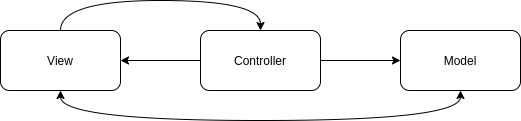
\includegraphics[width=\textwidth]{Chapters/img/2_background/mvc-pattern.jpg}
         \caption{MVC Pattern}
         \label{fig:mvc-pattern}
     \end{subfigure}
     \hfill
     \begin{subfigure}[b]{0.49\textwidth}
         \centering
         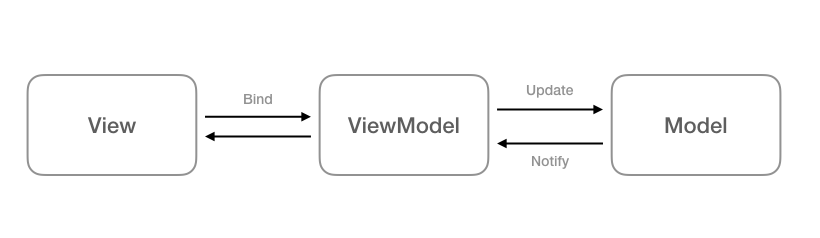
\includegraphics[width=\textwidth]{Chapters/img/2_background/mvvm-pattern.png}
         \caption{MVVM Pattern~\cite{mvvm-pattern-figure}}
         \label{fig:mvvm-pattern}
     \end{subfigure}
     \caption{Base architectural patterns}
\end{figure}

\acrlong{mvvm} (\acrshort{mvvm}) (Fig. \ref{fig:mvvm-pattern}) tried to solve this problem by tightly coupling views to a related ViewModel by having a two-way data binding for getting and setting values~\cite{mvvm-problems}. The ViewModel manages the Model data and the associated view using data bindings rather than through events, which makes it more predicable and easier to test.

At Facebook, models providing data to different views, views updating Models based on user interaction and Models updating other Models data, led to problems debugging the data flow when developing web applications~\cite{facebook-debugging-problems}. Flux suggests a solution to this by using an unidirectional data flow.

\begin{figure}[H]
	\centering
	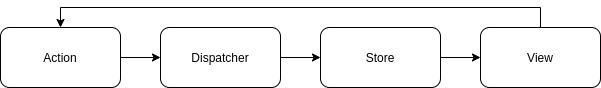
\includegraphics[width=1\linewidth]{Chapters/img/2_background/flux-pattern.jpg}
	\caption{Flux pattern}
	\label{fig:flux-pattern}
\end{figure}

The pattern consists of four elements:

\begin{itemize}
    \item \textbf{Stores} are where all the data in the application is located, only them can manipulate it. Information is exposed through public getters for views;
    \item \textbf{Views} can subscribe to stores and update accordingly. It is different from the MVC patterns where Views can update the data in the model freely;
    \item \textbf{Actions} are used to update data in the store. One Actions exists for every change needed in the application, it can happen due to a user interaction or a network request. Each Action is an object containing two fields: a \textbf{type} and a \textbf{payload}. The type is a unique string describing the action (e.g., ADD\_ESTATE). The payload field containers the data to update the Store. For an Action to reach a Store it goes through the Dispatcher;
    \item \textbf{Dispatcher} is responsible for handling incoming actions before passing them to the Store and deciding in which order the actions should be dispatched. By using actions, the operations are decoupled from the Views and can be reused for multiple Views.
\end{itemize}

\subsubsection{Vue}
\label{sss:vue}

Vue is a popular JavaScript framework that shares many similarities with React, it was created as a lightweight alternative to Angular and as such as many similar features but with less extra concepts. The core library of Vue focuses exclusively on the view layer and can be integrated with other libraries and projects, while also supporting complex \acrfull{spa}.

It uses an HTML based template syntax, it has a characteristic signature of declaring syntax using a "v-" prefix, which is its way of identifying Vue-specific attributes. An example of this are the two most used commands in Vue \textit{v-bind} and \textit{v-on}, which are used to bind data and to listen to events, respectively.

\subsection{Comparing frameworks}

All these frameworks have in common a component-based structure, by splitting the application into various independent parts, it allows developers to work on each individual function of the application asynchronously, thus leading to a more flexible development process, maintaining the same ideology we gained from the microservices.

Vue and React both use a virtual DOM, with VUE it consists of multiple virtual nodes that manage what information should be displayed and interacts with the real DOM to update the data on the HTML page, on the other hand React uses the virtual DOM to handle many of the rendering tasks using as little DOM manipulation as possible, thus decreasing the time and resources needed for updates. In contrast, Angular does not use a virtual DOM, instead it converts components into classes that can be displayed onto the DOM.

What sets React apart from the other frameworks is that React is only a UI library rather than a full-fledged Javascript framework like the other two. Which may seem like an disadvantage due to having less features, but actually makes it an optimal tool when the emphasis is on the interface.

For this reason, React was the winner library for this project due to its simplicity and freedom, which allowed us to focus on creating interfaces.

\subsection{Solution}
\label{ss:ui-solution}

The following sections describe the implementation details of the main features present in the frontend, created in React. Including some of the advantages of working with components, and how have we created our code to follow the flux design pattern. It is split into two main sections, the \textbf{user} and \textbf{zones}.

\subsubsection{User}
\label{s:user}

To register and authenticate users, we had to create multiple supporting pages. All these pages are mostly composed of simple forms, to assist with the validation and error handling we opted to use \textbf{Formik~\url{https://formik.org/}}, simplifying the creation process. 

\begin{figure}[H]
     \centering
     \begin{subfigure}[b]{0.49\textwidth}
         \centering
         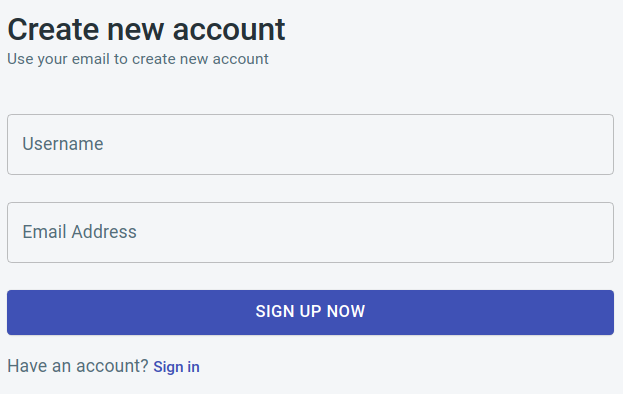
\includegraphics[width=0.8\linewidth]{Chapters/img/frontend/signUp.png}
    	\caption{Sign up}
    	\label{fig:signup}
     \end{subfigure}
     \hfill
     \begin{subfigure}[b]{0.49\textwidth}
         \centering
         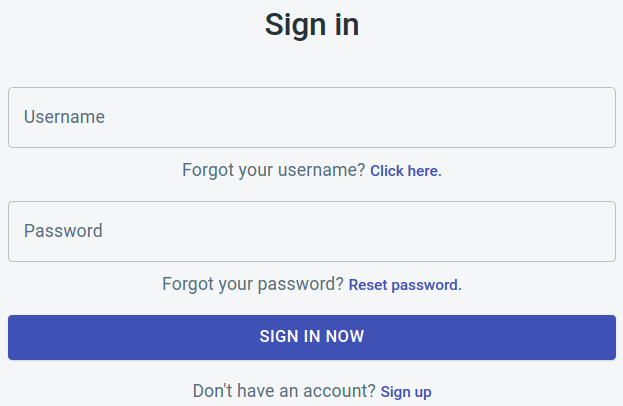
\includegraphics[width=0.8\linewidth]{Chapters/img/frontend/login.png}
	\caption{Sign in}
	\label{fig:signin}
     \end{subfigure}
     \caption{Registering and Authentication}
\end{figure}

\begin{figure}[H]
    \centering
    \begin{subfigure}[b]{0.49\textwidth}
        \centering
        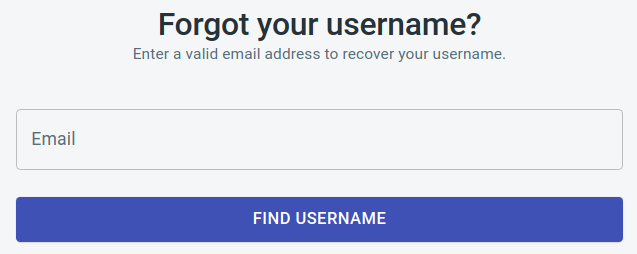
\includegraphics[width=0.8\linewidth]{Chapters/img/frontend/forgotUsername.png}
        \caption{Forgot username}
        \label{fig:forgotUsername}
     \end{subfigure}
     \hfill
     \begin{subfigure}[b]{0.49\textwidth}
        \centering
        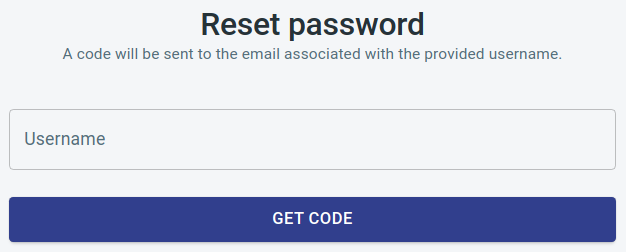
\includegraphics[width=0.8\linewidth]{Chapters/img/frontend/resetPassword.png}
        \caption{Reset password}
        \label{fig:resetPassword}
     \end{subfigure}
     \caption{Recovery}
\end{figure}

Upon creating an account, the user is prompted to fill out his profile. These components were designed in a way that would follow the \textbf{flux pattern} mentioned previously, which helps with the separation of concerns (rendering and state management). React provides the \textbf{useReducer()} hook that does so by extracting the state management out of the component. 

To understand the useReducer() hook it is necessary to first understand the following concepts:

\begin{itemize}
    \item \textbf{Initial State} is the value that the state is initialized with;
    \item \textbf{Action} is an object that describes how to update the state;
    \item \textbf{Dispatch} is a function that sends an action object;
    \item \textbf{Reducer} is a function that accepts 2 arguments, current state and an action. Based on the action, it must update the state in an immutable manner and return the new state.
\end{itemize}

\begin{figure}[h]
	\centering
	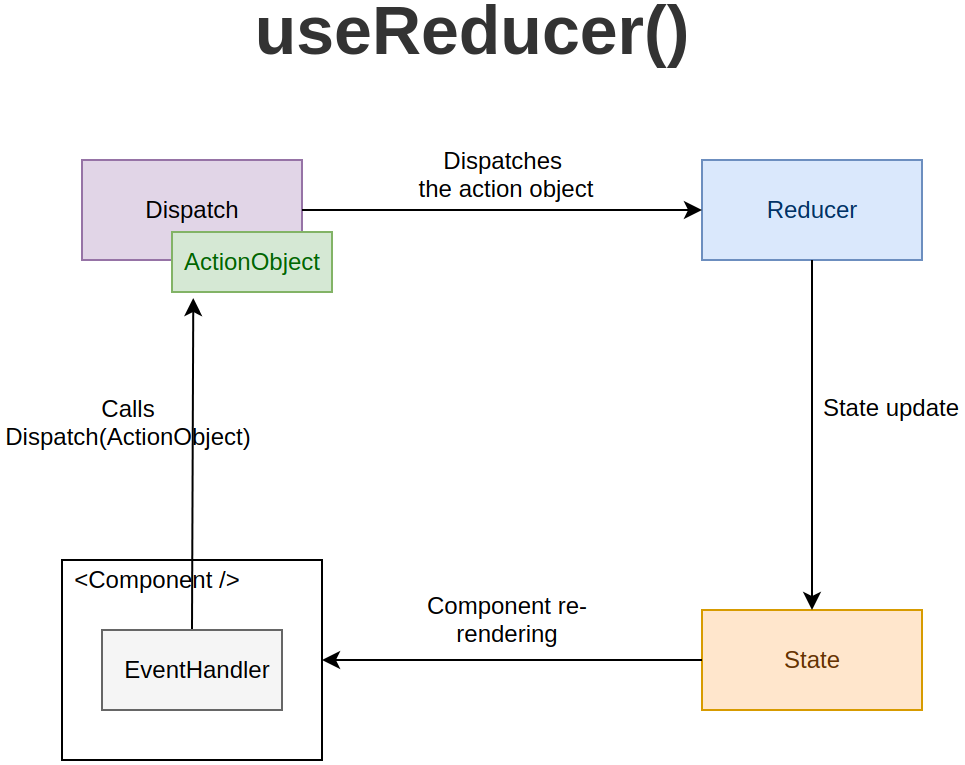
\includegraphics[width=0.5\linewidth]{Chapters/img/frontend/useReducer.png}
	\caption{useReducer() flow details~\cite{react-use-reducer}}
	\label{fig:useReducer}
\end{figure}

The diagram in Figure \ref{fig:useReducer} demonstrates the events that occur while using the useReducer() hook. Using the chip component (Fig. \ref{fig:ui-stepper-2}), used during the profile creation (Fig. \ref{fig:profile-stepper}). We start by capturing \textit{onClick()} events in the component, which are used to call the dispatch with an action to perform. In the following Listing (\ref{lst:dispatch}), the \textbf{ADD\_SELECTED\_FEATURE} was sent to the reducer.

%\begin{lstlisting}[language=Java, caption={EventHandler dispatching actions}, position={bottom}, label={lst:dispatch}]
\begin{lstlisting}[language=Java, caption={EventHandler dispatching actions}, label={lst:dispatch}]
const [state, dispatch] = useContext(FeaturesChipsContext);

const handleClick = (feature) => {

    if(state.selectedFeatures.length < MAX_FEATURES || feature.color == 'primary'){
        if(feature.color == 'default'){
            dispatch({
                type: "ADD_SELECTED_FEATURE",
                payload: {
                    feature: feature
                }
            });
        }
    ...
\end{lstlisting}

The reducer is implemented as a switch that updates the state according to the performed action, which for this action, alters the state by adding a new value to the selected feature list.

%\begin{lstlisting}[language=Java, caption={Reducer processing actions}, position={bottom}, label={lst:reducer}]
\begin{lstlisting}[language=Java, caption={Reducer processing actions}, label={lst:reducer}]
const [state, dispatch] = useReducer(reducer, initialState);

const reducer = (state, action) => {

    switch (action.type) {
        case "UPDATE_CHIPS":
            return {
                chips: action.payload.features
            };
        case "ADD_SELECTED_FEATURE":
            return {
                ...state,
                selectedFeatures: [...state.selectedFeatures, action.payload.feature.value]
            };
    ...
\end{lstlisting}

All the steps during the profile creation follow the same pattern. Taking advantage of having everything split into components, the same components are then reused in the preferences tab, where the user is allowed to update his preferences.

\begin{figure}[h]
	\centering
	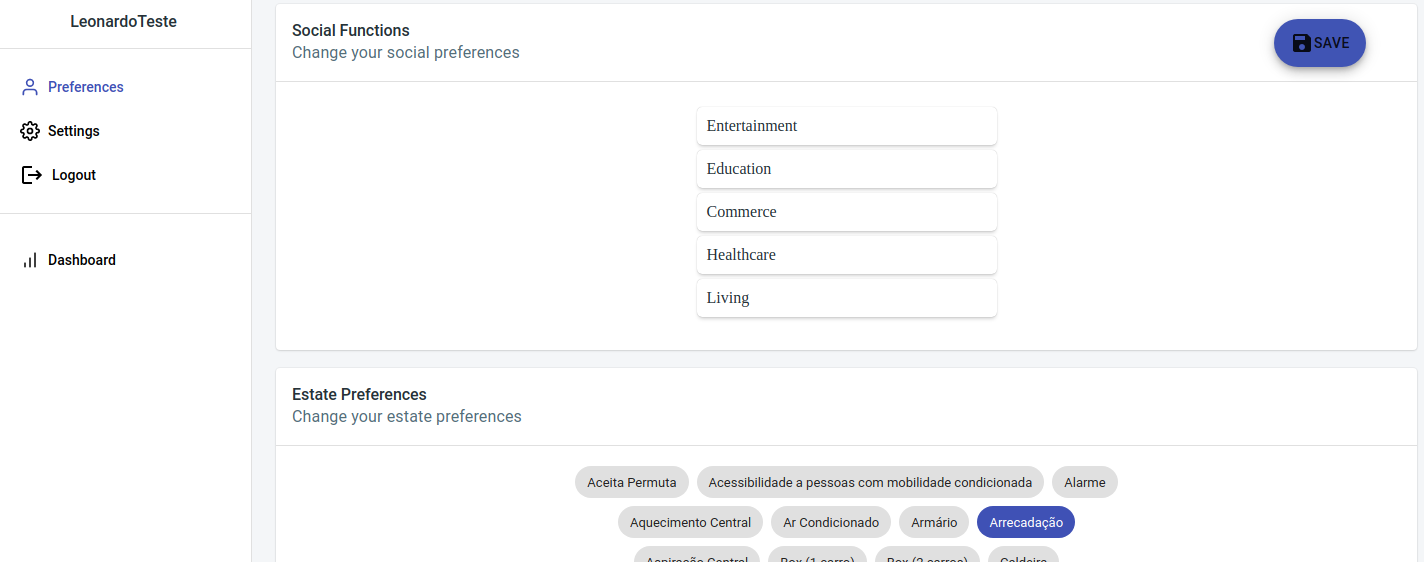
\includegraphics[width=0.6\linewidth]{Chapters/img/frontend/UserPreferences.png}
	\caption{Update user preferences}
	\label{fig:userPreferences}
\end{figure}

The same happens in the settings tabs, where the component used during the recovery process is used once again to change the password in a different context.

\begin{figure}[h]
	\centering
	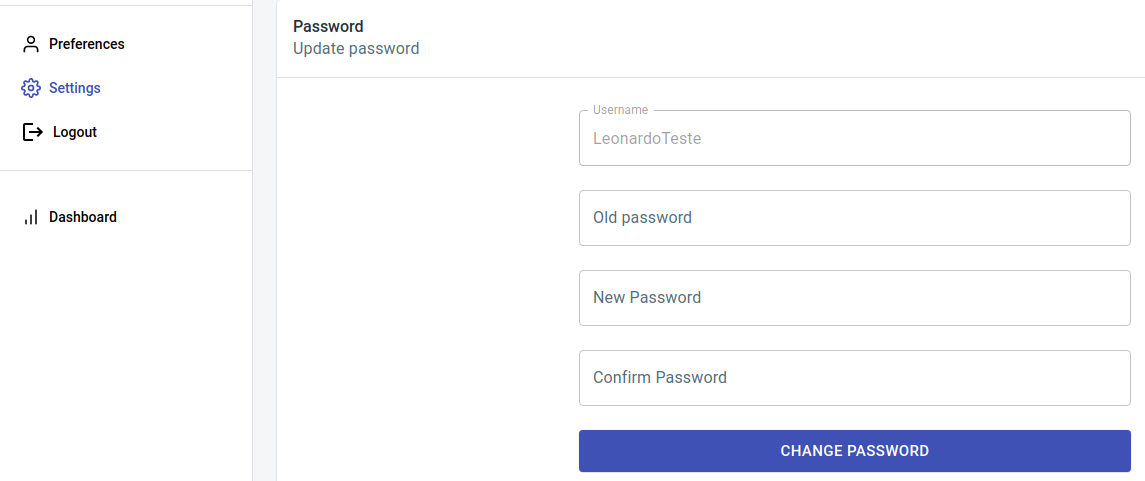
\includegraphics[width=0.6\linewidth]{Chapters/img/frontend/UserSettings.png}
	\caption{Update user settings}
	\label{fig:userSettings}
\end{figure}


\subsubsection{Dashboard} 
\label{sss:dashboard}

The dashboard is the main page of the application, when the user picks a new location to analyse, he is redirected to the dashboard. In the previous sections, while detailing the logic within the backend, it was shown how it looked (Figure \ref{fig:overviewDashboard}), now we will detail how each row was actually implemented in the frontend.

\paragraph{Zone overview} highlights some of the data gathered about the city such as the price and estate size. Most of the work for these information is done in the backend, and as such, there's nothing to highlight.

\begin{figure}[h]
	\centering
	
\includegraphics[width=1\linewidth]{Chapters/img/frontend/OverviewHeader.png}
	\caption{Random trivia about the selected zone}
	\label{fig:overviewHeader}
\end{figure}

\paragraph{Map} displays to the user several layers of geographical information composed of: \textbf{Points of Interest}, \textbf{Estates} and the \textbf{Zone}. It is built out of two different pieces, the header which includes multiple togglable buttons that allow the user to display only the relevant \acrshort{poi} and the map itself. As they both need to communicate, it was required to apply a technique known as \textit{Lifting State Up}, where a parent component was created to house both children, this way the parent is responsible for managing the estate of both subcomponents.

\begin{figure}[h]
	\centering
	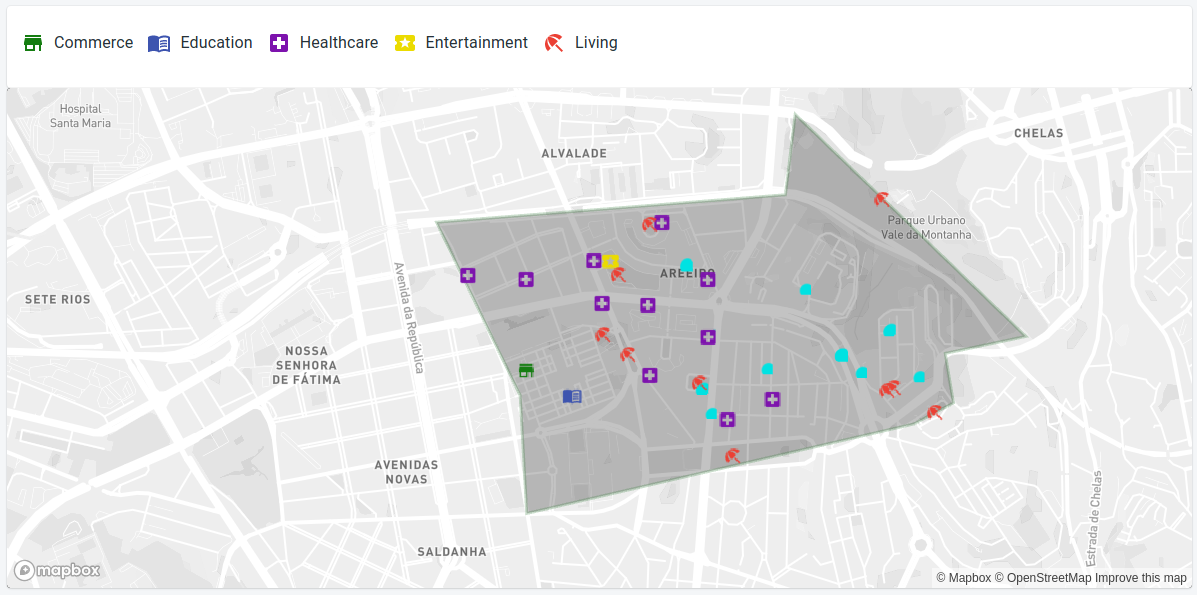
\includegraphics[width=1\linewidth]{Chapters/img/frontend/OverviewMap.png}
	\caption{Map}
	\label{fig:overviewMap}
\end{figure}

To control the state, the parent sends a callback function to the child component (handleCategoriesChange), allowing the map management component to handle the \textit{onClick()} events received within each button.

%\begin{lstlisting}[language=Java, caption={MapManagement component}, position={bottom}, label={lst:mapManagement}]
\begin{lstlisting}[language=Java, caption={MapManagement component},  label={lst:mapManagement}]
const handleCategoriesChange = (event) => {
    setState({ ...state, [event.target.name]: event.target.checked });
};

return <Grid item xs={12} width={'50%'} height={'50%'} >     
    <MapHeader onCategoriesChange={handleCategoriesChange} state={state}/>
     
    <Card style={{position: 'relative', background: 'black', minHeight:'500px'}}>
        <CardContent>
            <MapOSRM  locationId={localStorage.getItem('locationId')} locationType={props.zone.type} categories={getCatIds()}/>

            {/* <MapCluster /> */}
        </CardContent>
    </Card>
</Grid>
\end{lstlisting}

With the state handled by the manager component, it can be sent to the map component which can now render the selected social functions. To visualize the geospatial data we chose \textbf{deck.gl~\footnote{\url{https://deck.gl/}}} an open source geospatial analysis toolbox built by Uber on top of the Mapbox GL JS library, it is built to visualize massive datasets without compromising performance (e.g., Uber hundreds of millions of trips). For the application use-case, their layered approach to data visualization turned out to be extremely valuable, allowing us to render all of our three layers of data separately and improve the user experience as the user is presented some of the data while the rest is rendering.

%\begin{lstlisting}[language=Java, caption={Example of a GeoJSON layer, used to represent the zone geometry as seen in Fig. \ref{fig:overviewMap}}, label={lst:mapLayer}, position={bottom}]
\begin{lstlisting}[language=Java, caption={Example of a GeoJSON layer, used to represent the zone geometry as seen in Fig. \ref{fig:overviewMap}}, label={lst:mapLayer}]
new GeoJsonLayer({
      id: 'polygon-layer',
      data: zoneGeometry.then(data => data.data),
      pickable: false,
      stroked: true,
      filled: true,
      wireframe: true,
      opacity: 0.05,
      lineWidthMinPixels: 3,
      getLineColor: d => randomColor(),
      getFillColor: [20, 20, 20],
      getLineWidth: 3
})
\end{lstlisting}

The Listing \ref{lst:mapLayer} shows an example of such layers, a promise is passed on to the data field which waits for it be fulfilled to it can be rendered and displayed to the user. This layer, along with all others, is then passed on to the \textbf{DeckGL} component, additionally a tooltip is added to each element to display some relevant information according to its type.

%\begin{lstlisting}[language=Java, caption={Map JSX returned by the component}, label={lst:mapJSX}, position={bottom}]
\begin{lstlisting}[language=Java, caption={Map JSX returned by the component}, label={lst:mapJSX}]
return  <DeckGL
    initialViewState={viewState}
    controller={mapController}
    layers={layers}
    getTooltip= {({object}) => object &&
        `${object.properties.metadata != null 
            ? 
            'Name: ' + object.properties.metadata.INF_NOME + '\n' +
            'Description: ' + object.properties.metadata.INF_DESCRICAO + '\n' +
            'Address: ' + object.properties.metadata.INF_MORADA + '\n' 
            : 
            'Price: ' + object.properties.value + '\n' +
            'Typology: ' + object.properties.typology + '\n' + 
            'Living Area: ' + object.properties.living_area + '\n' +
            'Gross Area: ' + object.properties.gross_living_area + '\n' +  
            'Construction Year: ' + object.properties.construction_year + '\n'
        }`
    }
    width={'100%'}
    height={'100%'}
    >
      <MapView id="map" >  
        <StaticMap mapboxApiAccessToken={MAPBOX_ACCESS_TOKEN} />
      </MapView>
    </DeckGL>;
\end{lstlisting}

\paragraph{Zone information} presents to the user some relevant data about the estates in the selected area, such as common features and number of bedrooms, commonly refered as Typology in Portugal. This components are supported by the \textbf{Nivo~\footnote{\url{https://nivo.rocks/}}} library, a collection of React components built on top of d3~\footnote{\url{https://d3js.org/}} that facilitate the process of creating charts.

\begin{figure}[h]
	\centering
	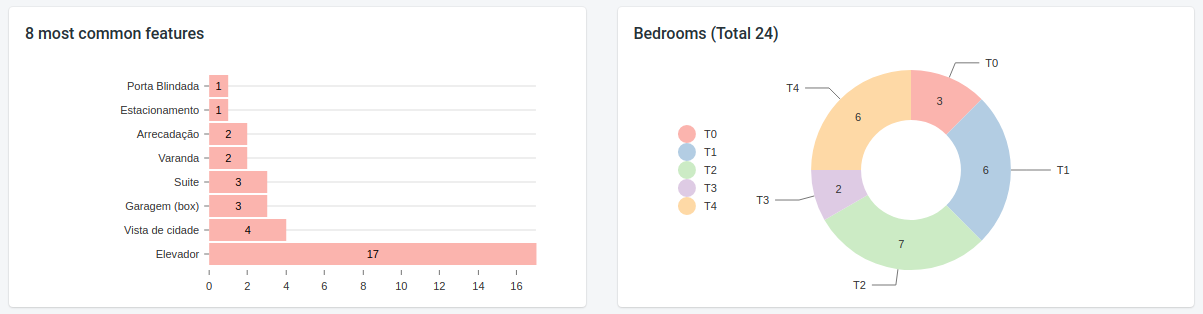
\includegraphics[width=1\linewidth]{Chapters/img/frontend/OverviewEstateData.png}
	\caption{Information about the estates in the zone}
	\label{fig:overviewSearchBar}
\end{figure}

\paragraph{Estates} is the most important section of the dashboard, right after the map, as it allows the user to browse each estate and see his personalized index associated with each estate. The table allows the user to select the number of estates to display per page, sort the estates by the numerous fields, numerically or alphabetically, while also allowing the user to filter results by pressing the header and entering out their queries (e..g., price > 10).

\begin{figure}[h]
	\centering
	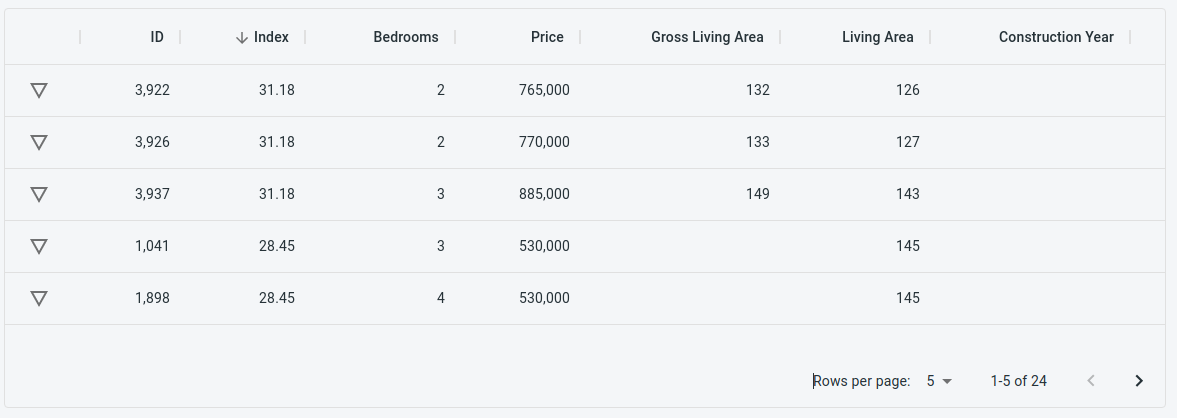
\includegraphics[width=1\linewidth]{Chapters/img/frontend/OverviewEstateListIndex.png}
	\caption{List of estates in the selected zone}
	\label{fig:overviewListEstate}
\end{figure}

Additionally, each row is accompanied by a triangle, this symbol represents the ability to expand each estate and learn more about it.

\begin{figure}[h]
	\centering
	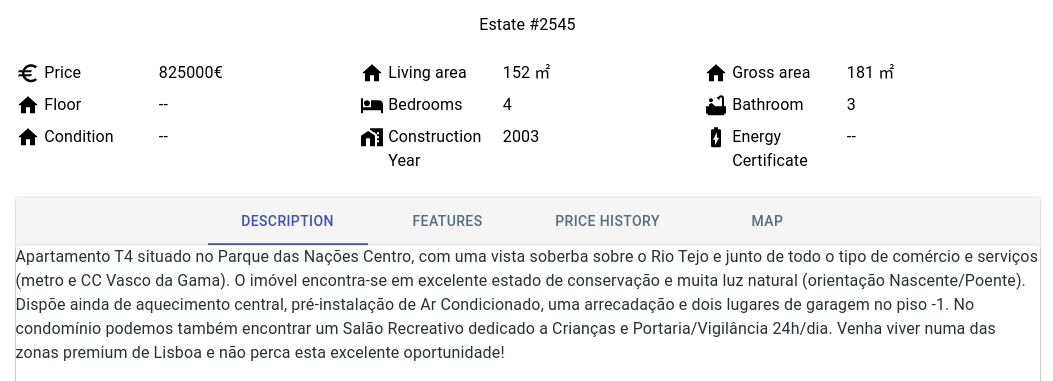
\includegraphics[width=1\linewidth]{Chapters/img/frontend/DetailedDescription.png}
	\caption{Estate list data}
	\label{fig:detailed}
\end{figure}

In this modal (window popup), the user can read the original description extracted during the scraping, the features associated with each estate, the price history with the scraped price after each iteration, and the location of the estate in the map, but unlike the previous map the zone shown actually represents the area the user can reach with the selected travel mode in 15 minutes, along with all containing points of interest (even the ones that do not belong to the current selected zone). 

\begin{figure}[H]
    \centering
    \begin{subfigure}[b]{0.49\textwidth}
        \centering
        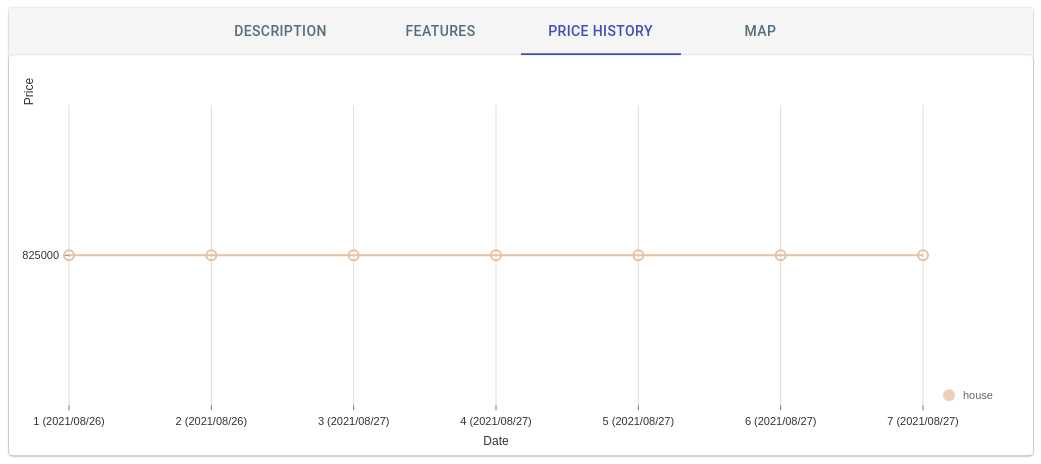
\includegraphics[width=1\linewidth]{Chapters/img/frontend/DetailedPriceHistory.png}
        \caption{u}
        \label{fig:detailedPriceHistory}
     \end{subfigure}
     \hfill
     \begin{subfigure}[b]{0.49\textwidth}
        \centering
        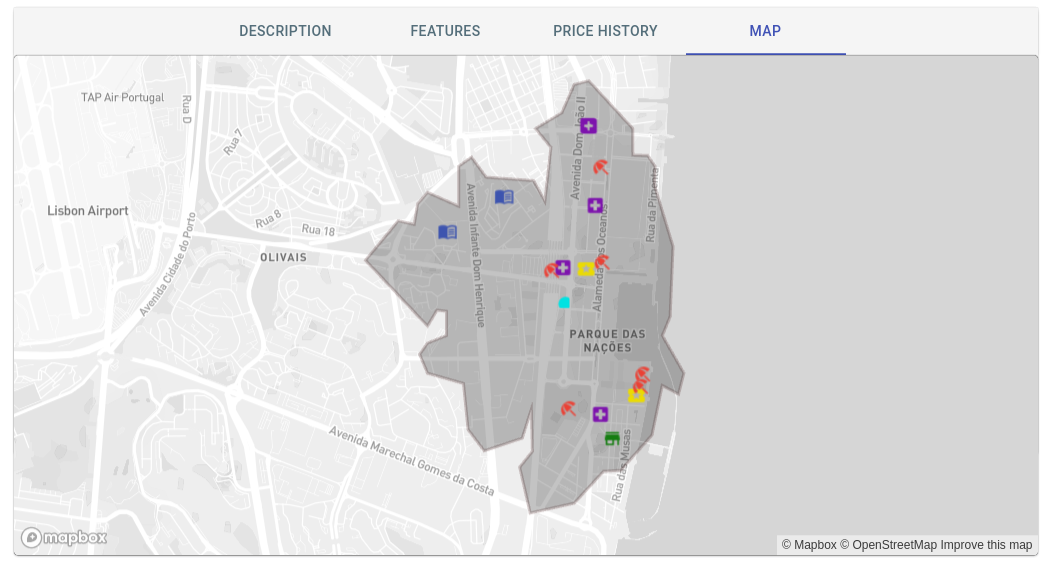
\includegraphics[width=1\linewidth]{Chapters/img/frontend/DetailedIsochrone.png}
        \caption{r}
        \label{fig:detailedIsochrone}
     \end{subfigure}
     \caption{Tabs of detailed view}
\end{figure}



\section{Monitoring}
\label{s:monitoring}

%\chapter{Monitoring}
%\label{ch:monitoring}

%One of the disadvantages of a microservice architecture is the amount of information it produces and requires the user to keep up with.
With the growth of the microservices industry, and as a new way of constructing applications, microservices' availability, performance, and functionality becomes a concern that everyone cares about. Stakeholders want to make sure each end-user has a good experience, operations teams want to ensure applications are available and performing well, and development teams want the applications and microservices to function as designed.

Even though everything most services are decoupled, some still rely on communication between them and as such, if a component deteriorates or fails, it can still affect the applications performance or eventually lead to application failure. Understanding how each component is performed is essential to gauge the real health and status of the application as a whole. This monitoring can help the team:

\begin{itemize}
    \item Understand the overall health of the application
    \item Gain insight into the performance of each individual service
    \item Ensure that transactions are available and performing well
    \item Understand the load of each service (i.e., maybe a feature is not being used and can be replaced by something else or removed entirely)
    \item Optimize end-user experience
\end{itemize}

However, gathering all these metrics and reading them from massive text files still does not solve the problem at hand. As such, visualization tools were introduced, which allow for an easier real-time overview of data. This tools consume the logs produced by the monitoring tools and allow the exploration of such data with filtering and grouping. For example, instead of having the current number of users constantly updated without having a way to see previous values, we can now trace a graph of concurrent users which allows us to understand how it is progressing.

The following section \ref{ss:monitoring-implementations} will detail some of the tools currently available for monitoring and visualization, followed by an description of how they were integrated into our system in Section \ref{ss:monitoring-solution}.

%\subsection{Problem}
%\label{s:6_problem}

\subsection{Implementations}
\label{ss:monitoring-implementations}

The following sections describe the tools found that could aid us with the monitoring process and everything the precedes it such metric scraping and the tools to helps us visualize all of this information.

\subsubsection{Prometheus}
\label{sss:prometheus}
%% -- Created: 03-07-21
%% -- Last edit: 05-07-21

Prometheus \footnote{\url{https://www.prometheus.io/}} is an open-source monitoring system which collects metrics, evaluates expressions, offers visualization dashboards and has alert mechanisms. Its main features are~\cite{prometheus-overview}:

\begin{itemize}
    \item A multidimensional data model with time series data identified by metric name and key/value pairs (e.g. <metric name>\{<label name>=<label value>, ...\});
    \item \textbf{PromQL} a flexible query language to leverage this dimensionality;
    \item Autonomous single server nodes, as such, no reliance on distributed storage;
    \item Time series collections occurs via a \gls{pull-model} over \acrshort{http};
    \item Monitored nodes (targets) are discovered via service discovery or static configuration
\end{itemize}

\paragraph{Architecture}
%\label{sss:prometheus-architecture}

The prometheus ecosystem consists of multiple components, some of which can see be seen in Fig. \ref{fig:prometheus-architecture}.

\begin{figure}[h]
    \centering
    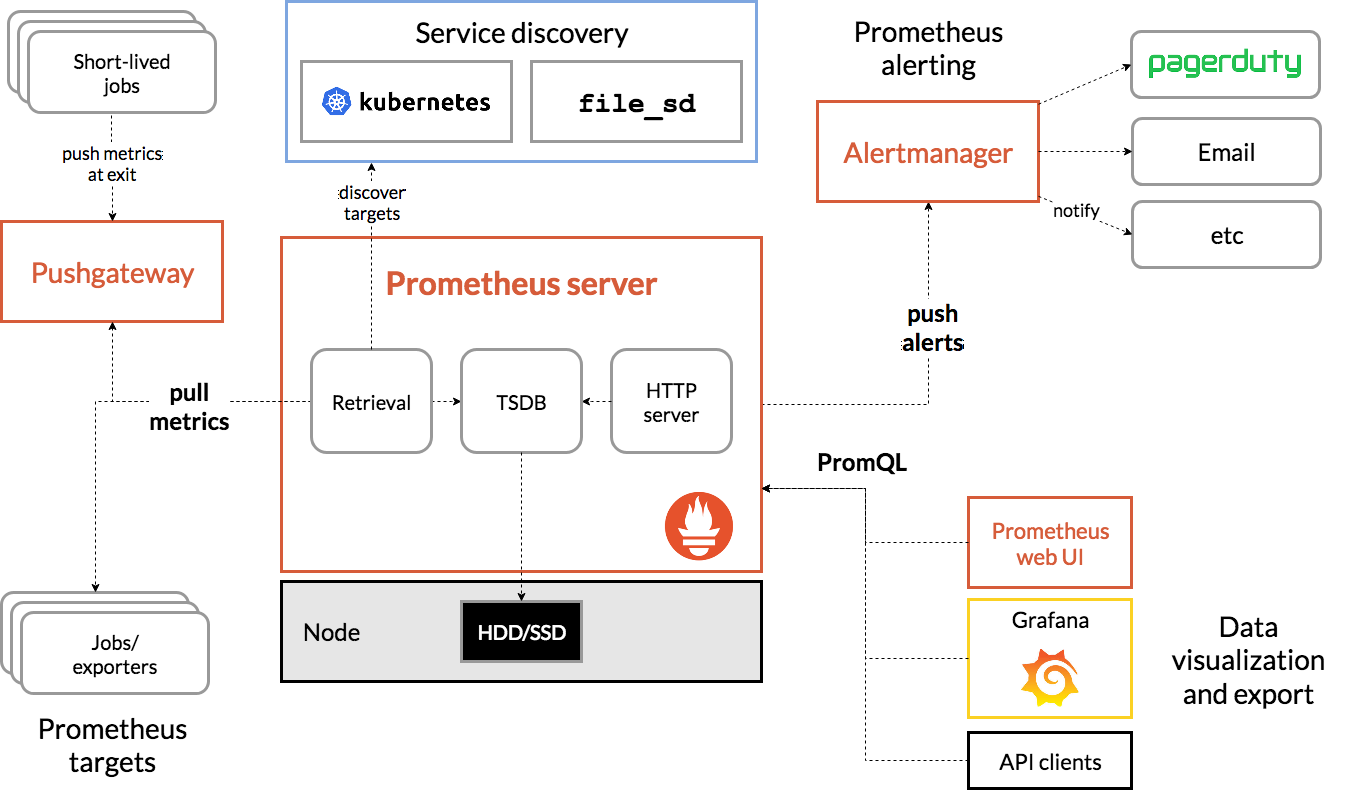
\includegraphics[width=1\textwidth,clip,trim=0 0 0 0]{Chapters/img/2_background/prometheus-architecture.png}
    \caption{Prometheus architecture~\cite{prometheus-overview}} 
    \label{fig:prometheus-architecture}
\end{figure}

The main components are:

\begin{itemize}
    \item \textbf{Prometheus server:} scrapes metrics from one or more targets and stores them in a \acrlong{tsdb} (\acrshort{tsdb});
    \item \textbf{Client-libraries:} there are multiple available libraries to match the language used in the application, that let the user define and expose internal metrics via an \acrshort{http} endpoint on the application instance;
    \item \textbf{Push gateway:} Support short-lived jobs, who push communication to announce their metrics. Since these kind of jobs may not exist long enough to be scrap, they are pushed to the push gateway, who then exposes these metrics to prometheus; 
    \item \textbf{Exporters:} monitor third-party systems to convert the existing metrics into the prometheus data model;
    \item \textbf{Alertmanager:} Handles alerts sent by client applications such as the Prometheus server. It takes care of deduplicating, grouping and routing them to the correct third-party notification platforms such as email.
    
\end{itemize}

Prometheus was chosen due to its popularity in the industry and for being an open-source project. It can easily be customized to our needs if required, and most of all its easy to scrape metrics from other software allowing for easier integration with the current system.


%------------------------------------------%------------ Grafana -----------------------------
\subsubsection{Grafana}
\label{sss:grafana}
%% -- Created: 03-07-21
%% -- Last edit: 05-07-21

Grafana~\footnote{\url{https://grafana.com/}} is a cross platform open-source measurement, analysis and visualization tool, which can query the collected data and present it through multiple dashboards. 

Grafana monitoring is achieved using panels, which is the basic building block for visualization in Grafana, and those panels can contain graphs, tables, text, or custom plugins (i.e. a clock or map). As such, a dashboard is a collection of panels, each of which holds a set of variables (server, application, sensor name) arranged in a grid, which the user can change the observed data by switching variables. An example of a dashboard can be seen in Fig. \ref{fig:grafana-example}.

\begin{figure}[h]
    \centering
    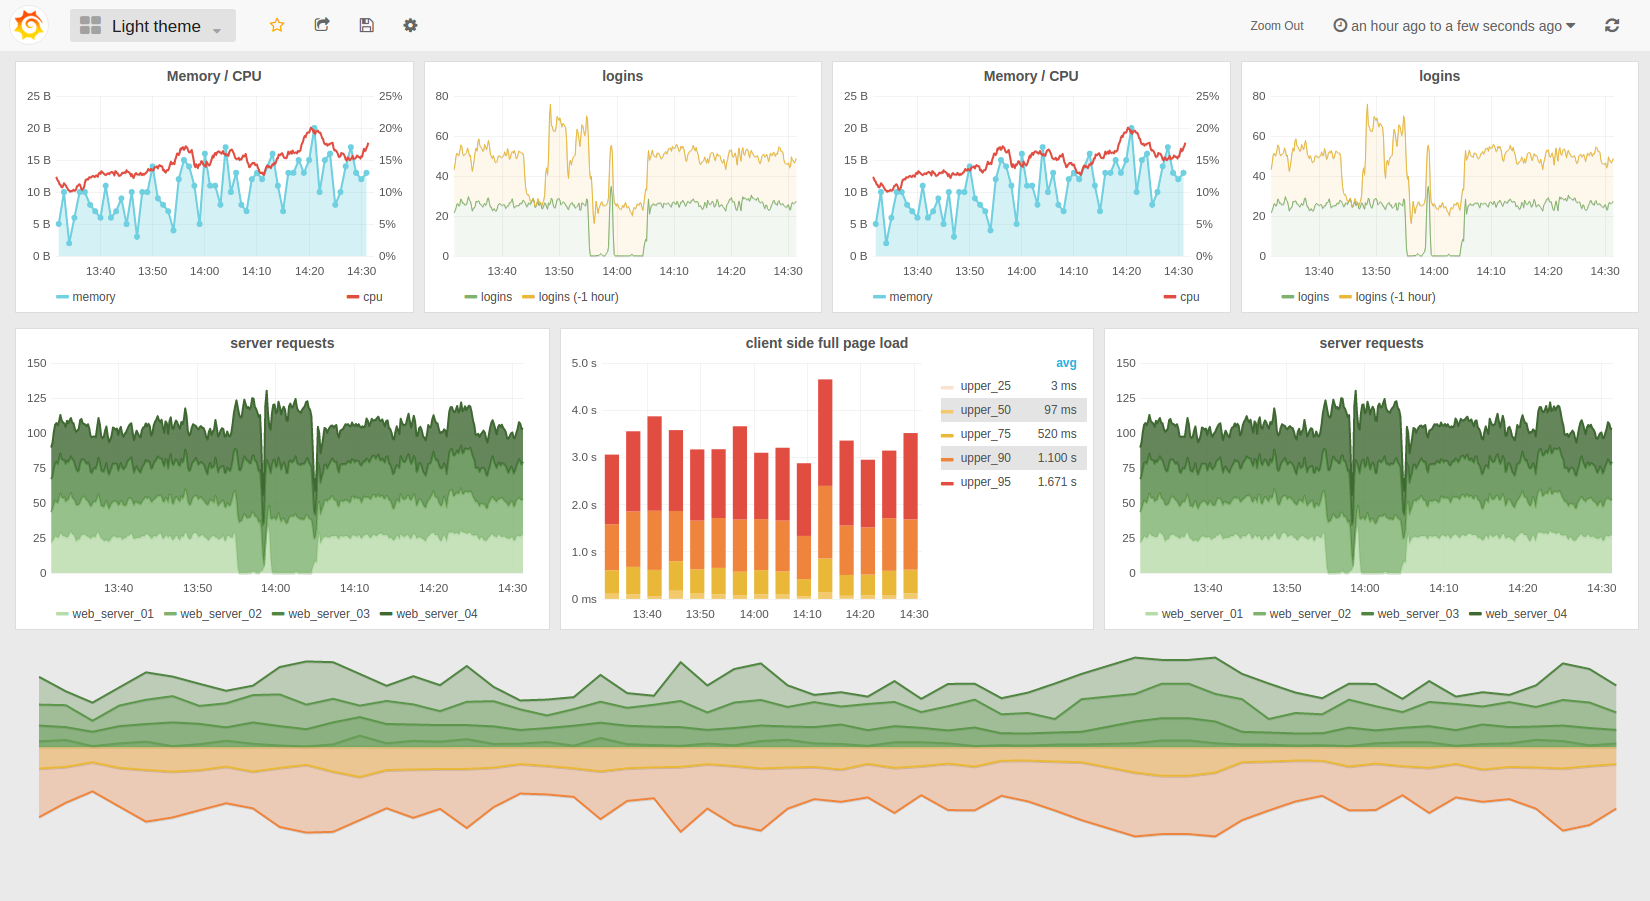
\includegraphics[width=1\textwidth,clip,trim=0 0 0 0]{Chapters/img/2_background/grafana-example.png}
    \caption{Grafana dashboard~\cite{grafana-example}} 
    \label{fig:grafana-example}
\end{figure}

Its main features are~\cite{grafana-features}:

\begin{itemize}
    \item \textbf{Dashboard templating}: It allows the users to create a dashboard to suit their needs, without almost no restrictions, they are extremely adaptable. Templating lets data be examined at every level from macro to micro (e.g., starting with a whole country and drilling down to a particular region). The dashboards are then shareable with everyone;
    \item \textbf{Provisioning:} It provides provisioning so the setup can be automated using a script. For instance, to create a new Kubernetes cluster, it is possible to have Grafana automatically help with a script that already has the right server, IP address, and data sources set up and locked;
    \item \textbf{Annotations:} It is possible to manually annotate data, which is particularly helpful to correlate data when something goes wrong; 
    \item \textbf{Kiosk mode}: dashboards can be selected to create a playlist, this playlist can now be displayed in a TV or monitor to cycle throughout the day;
    \item \textbf{Teams and permissions:} Dashboards can be limited to specific teams, allowing only determined dashboards to be viewed by teams in charge of that service.
\end{itemize}

One of the most common alternatives to Grafana is \textbf{Kibana}~\footnote{\url{https://www.elastic.co/kibana/}}, where the key difference between the two tools stems from their purpose. Grafana design caters to analyzing and visualizing metrics such as memory, CPU, disk, and I/O utilization. It does not allow full-text data querying. Kibana, on the other hand, runs on top of Elasticsearch and is used primarily to visualize and analyse log messages. They are both useful in their respective fields, but for this thesis Grafana served our needs better.


\subsection{Solution}
\label{ss:monitoring-solution}

%Even though there were multiple relevant sections to monitor such as databases, code itself through logs, etc... We chose to focus on the well-being and performance of the microservices themselves.
%Começamos por monitorizar os microserviços associados ao backend, criados em Java.

Even through it was possible to monitor and track the entire system, we have decide to focus our efforts on the well-being and performance of backend microservices. Which means we care about what is happening on the pods that are hosting our services. 

Instead of manually exposing each of the resources and setting up each microservice individually, we chose to use the \textit{Spring Boot Actuator}, which adds features to help monitor the service, gather metrics, understand traffic, and even state of the database, all exposed through HTTP endpoints. It includes several endpoints and the possibility of adding custom ones. For the current goal, the following endpoints were considered as the most important:

\begin{itemize}
    \item \textbf{health} shows application health information, such as \textbf{readiness state} which tells whether the application is ready to accept client requests and \textbf{liveness state}, which indicates whether the internal state is valid, if it is broken it means the application itself is in a failed state and cannot recover from it;
    \item \textbf{metrics} shows 'metrics' information for the current application with the support of the Micrometer~\footnote{\url{https://micrometer.io/}} library, an instrumentation library for JVM-based applications designed to add little to no overhead to the metrics collection activity;
    \item \textbf{prometheus} which exposes metrics in an format that can be scraped by a Prometheus server, once again provided by the micrometer library, as it provides a simple facade over the instrumentation clients for the most popular monitor systems, namely Prometheus.
\end{itemize}

Prometheus is then configured to scrape or poll individual app instances for metrics exposed in \textit{/actuator/prometheus}. For this we must create a \textit{scrape configuration}, which specify a set of targets and parameters describing how to scrape them, also known as \textit{jobs}. Listing \ref{lst:prom-params} provides an example of a job created to scrape the actuator metrics from the \textbf{Params} microservice.

\begin{lstlisting}[caption={Prometheus job for params microservice}, label={lst:prom-params}, captionpos=b]
- job_name: 'be-params-actuator-prometheus'
  metrics_path: '/actuator/prometheus'
  scrape_interval: 5s
  static_configs:
  - targets: ['10.111.42.84:8086']
    labels:
      namespace: backend
      pod: be-params-deployment
      service: be-params-services
\end{lstlisting}

%These metrics can then be utilize by Prometheus, which is constantly performing requests to the API and acquiring data. On top of this metric, we can now apply aggregation queries with \textit{PromQL}, which allowed us to retrieve information such as average requests during the last five minutes. 

%\todo[inline]{Mostrar exemplo de uma query e se for preciso mudar o exemplo dado}

However, one of the reasons which led us to implement and expose this metrics is so we could make them readable by \acrshort{k8s}, allowing us to manage the cluster resources in a more efficient manner reacting to the live feed of information, which is made possible with tools such as the \acrshort{hpa}. But, as mentioned previously, the \acrshort{hpa} only works, by default, with metrics provided by \acrshort{k8s} such as CPU and RAM usage. For this reason, we had to use the third party library \textbf{Prometheus Adapter}~\footnote{\url{https://github.com/kubernetes-sigs/prometheus-adapter}}, which when configure allows the \acrshort{k8s} cluster to recognize the metrics made available through Prometheus. 

The adapter determines which metrics to expose, and how to expose them, through a set of "discovery" rules, where each rule is executed independently, and specifies each of the steps the adapter needs to take to expose a metric in the API. The rules can be broken down into four parts:

\begin{itemize}
    \item \textbf{Discovery}, which specifies how the adapter should find all Prometheus metrics for this rule;
    \item \textbf{Association}, which specifies how the adapter should determine which \acrshort{k8s} resources a particular metric is associated with;
    \item \textbf{Naming}, specifies how the adapter should expose the metric in the custom metrics API;
    \item \textbf{Querying}, which specifies how a request for a particular metric on one or more \acrshort{k8s} objects should be turned into a query to Prometheus.
\end{itemize}

An example of such rules can be seen in Listing \ref{lst:prom-adapter-conf}, which highlights the four parts mentioned: discovery is done through the \textit{seriesQuery}, which specifies the Prometheus series query to use to find some set of Prometheus series; association is controlled by the \textit{resource} field, for this specific case with was done through its kubernetes namespace (backend); naming, the process of converting a prometheus metric name into a metric in the custom metrics API, is controlled by the \textit{name} field; and finally, querying through the \textit{metricsQuery} field, which is a Go template that gets turned into a Prometheus query, for this specific an aggregation query was performed with \textit{PromQL}, which used a rate function over a specific metric with information from the previous three minutes, more details will be provided on this later on during the Testing section (\ref{s:testing}).

\begin{lstlisting}[caption={Prometheus adapter configuration}, label={lst:prom-adapter-conf}, captionpos=b]
    - seriesQuery: '{__name__=~"^http_server_requests_seconds_max"}'
    resources:
      overrides:
        namespace:
          resource: namespace
    name:
      matches: "^(.*)_max"
      as: "http_server_requests_seconds_max_rate"
    metricsQuery: 'rate(http_server_requests_seconds_max{uri=~"/v1/params.*"}[3m])'
\end{lstlisting}

All of this became useful while trying to automate the entire system, however personal oversight is also important, and as such, all information was made available for visualization and analysis through Grafana, which unlike \acrshort{k8s}, pairs up easily with Prometheus.

In Grafana, we can now set up dashboards for each microservice with multiple panels displaying information we deem relevant extracted directly from Prometheus. In Fig. \ref{fig:grafana-dashboard} it is possible to observe our main configuration during testing, which allows us to track and understand the performance of our service, from requests received to garbage collector performance. 

A more in-depth explanation of how the setup was used will be given in the \textit{Testing} section (\ref{s:testing}), where it was crucial for setting up the cluster resources. 

\begin{figure}[h]
    \centering
    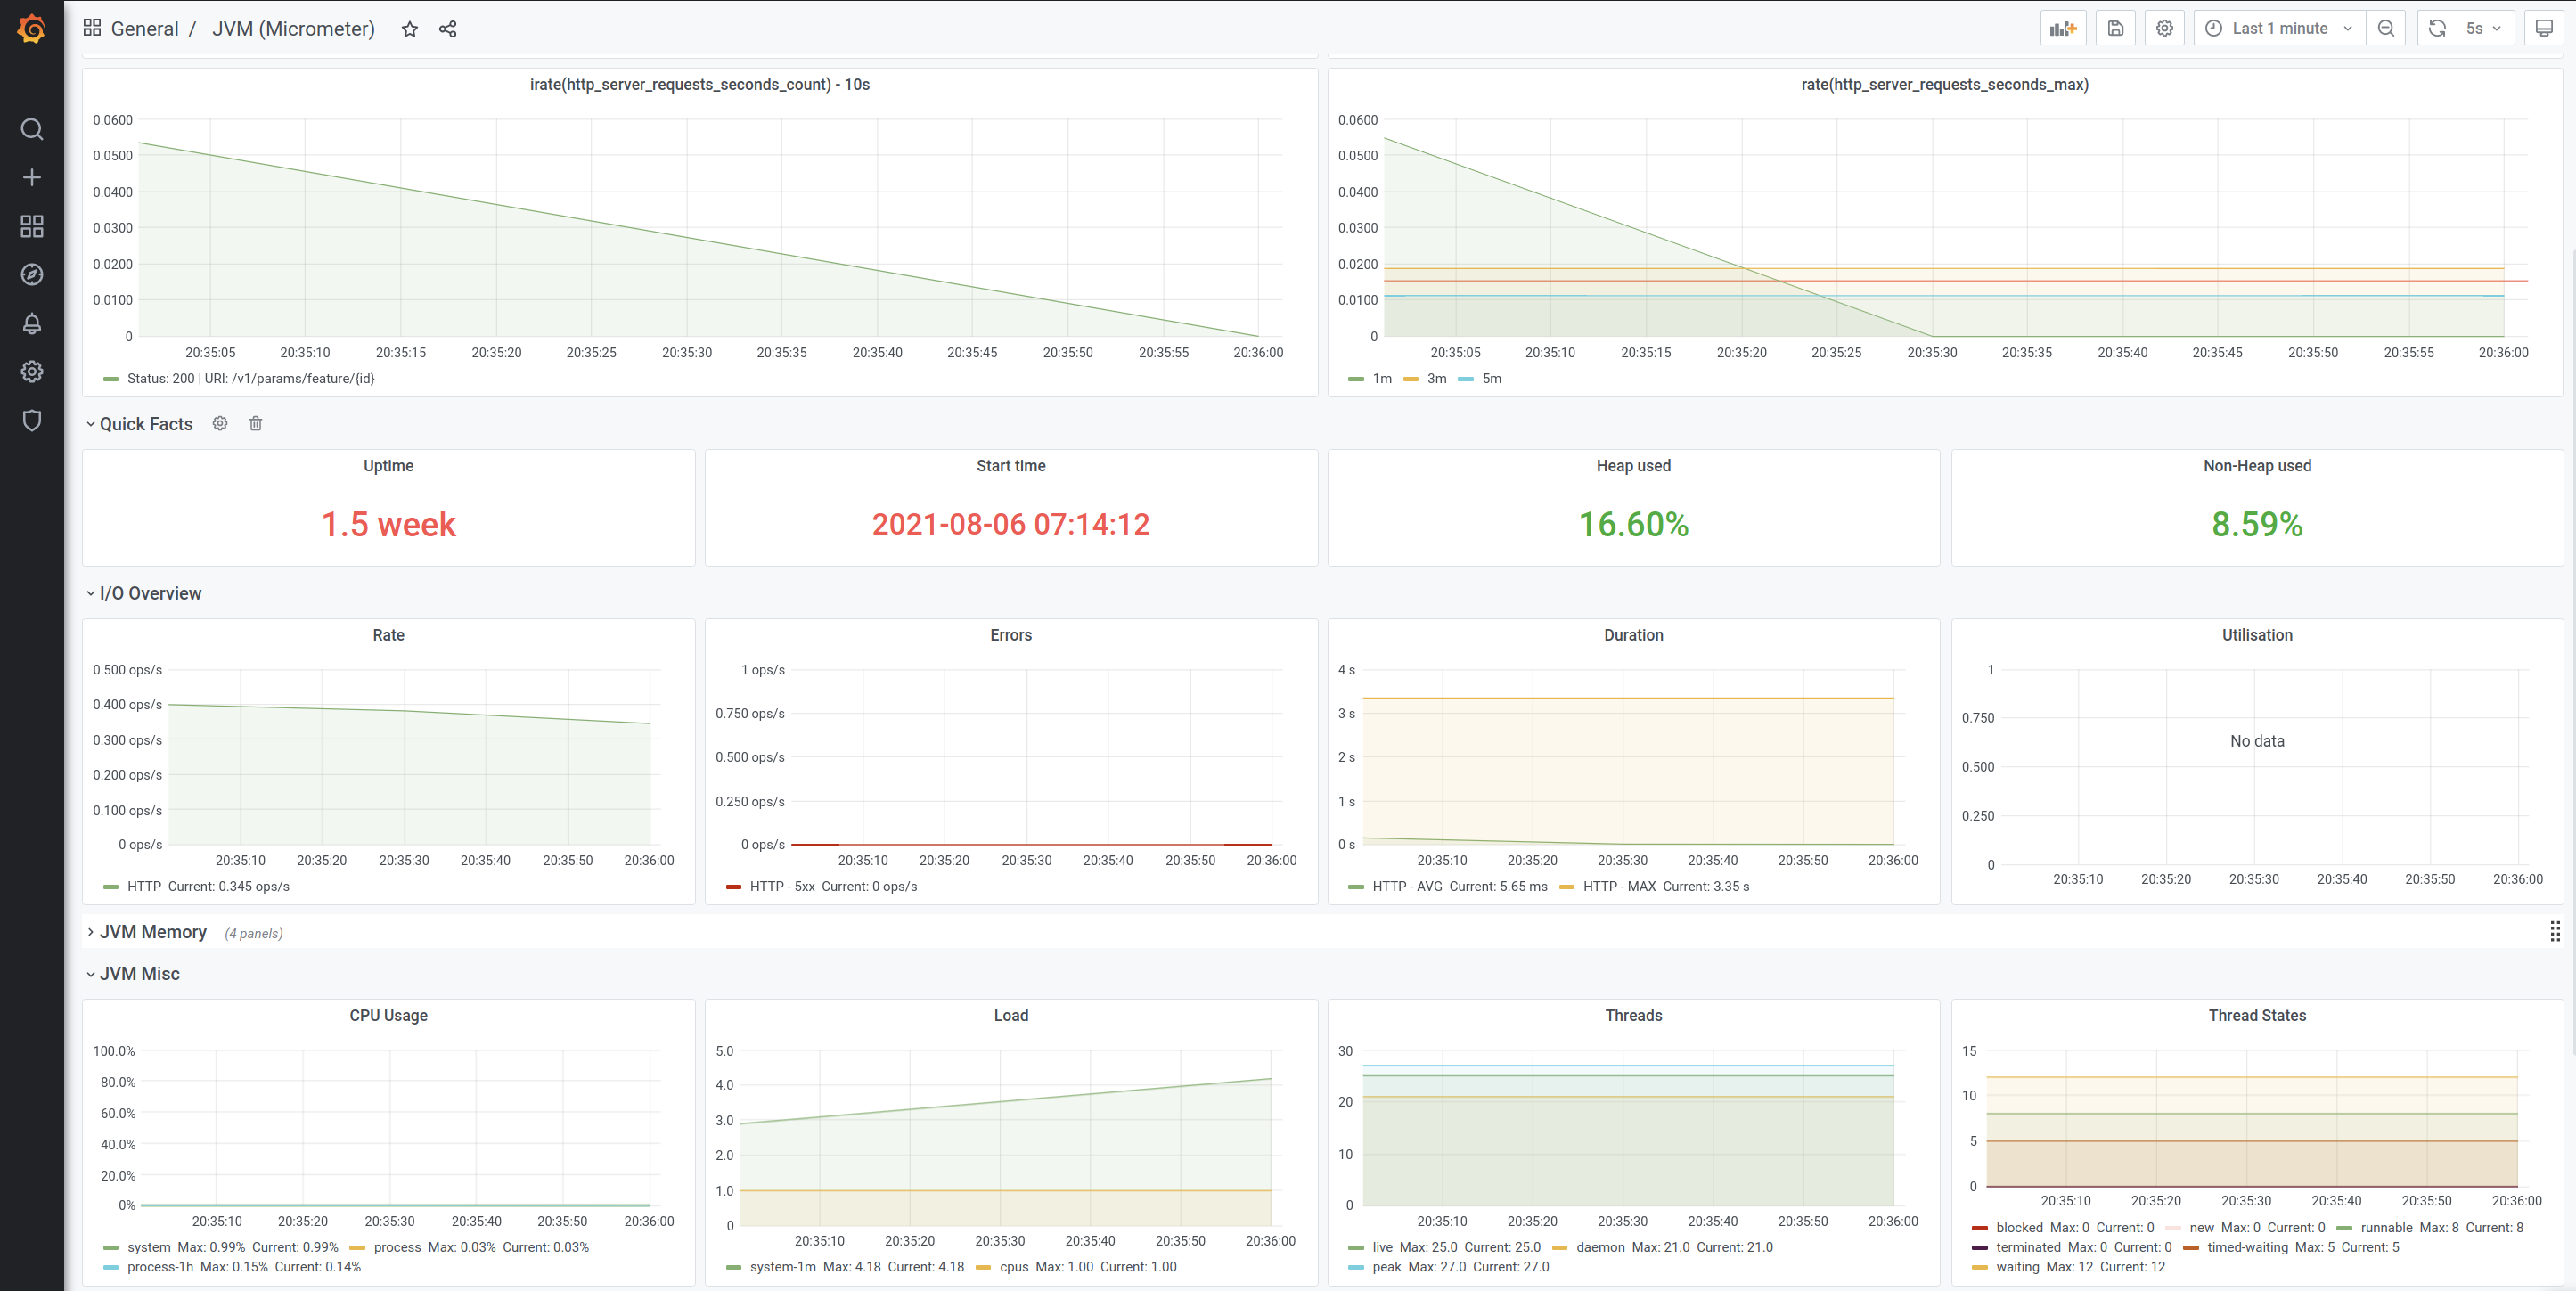
\includegraphics[width=1\textwidth,clip,trim=0 0 0 0]{Chapters/img/backend/grafana-dashboard.png}
    \caption{Grafana dashboard} 
    \label{fig:grafana-dashboard}
\end{figure}



%\chapter{Testing}
%\label{s:testing}

%\chapter{Testing}
\label{ch:testing}

There are multiple ways to evaluate an application, such as functional tests that aim to validate how each application function operates in accordance with the requirements of its specification. Essentially, each functionality is tested with an appropriate input, observing its results and comparing them with the expected output. Alternatively, there are non-functional tests, which aim to test the performance of the application (scalability, use of resources) when it is subject to different conditions.

For nonfunctional testing, \textbf{Apache JMeter}\footnote{See \href{https://jmeter.apache.org/}{jmeter.apache.org}} was picked as the tool of choice, commonly used to load test applications and measure system performance.

All the JMeter tests were performed in a laptop with 6 cores and 32GB of RAM, while all microservices were running in a cluster with 12 cores and 24GB of RAM.


\subsection{Non-functional}
\label{s:non-functional}

As a proof-of-concept, stress tests focused solely in one of the microservices, \textbf{Parameter}, with the goal
of discovering the maximum number of users the system is capable of accommodating and discovering the thresholds that allow the system to properly scale up and down while providing a consistent and stable user experience, despite the number of simultaneous users.

As stated previously, tests were created with \textit{JMeter}, as it allows the setup of multiple testing scenarios with different numbers of users, ramp-up periods, and duration. As the goal was to understand how many users could the system serve at a given time, it was first required to understand the limit of users for one and two instances. Based on those results, we should be able to extrapolate the best metric to setup automatic scaling between scenarios with one and two pods.

To make the tests consistent, they all had a ramping period of 60 seconds, where users are added periodically followed by a 240 seconds period of user interaction. As this application has no critical functionality, where losing requests has no consequences besides a bad user experience, tests with a minimum of 98\% success rate were considered successful.

Results wise, as depicted in the Fig.~\ref{fig:1pod} to \ref{fig:metric_max}, each circle is the result of an average of 5 tests, all done under the same circumstances for the specific situation being tested. The tests were performed over four phases, each iterating on the previous one, as seen in Figures~\ref{fig:1pod} and \ref{fig:2pods}.

\begin{figure}[t] 
  \label{fig7} 
  \begin{minipage}[b]{0.5\linewidth}
    \centering
    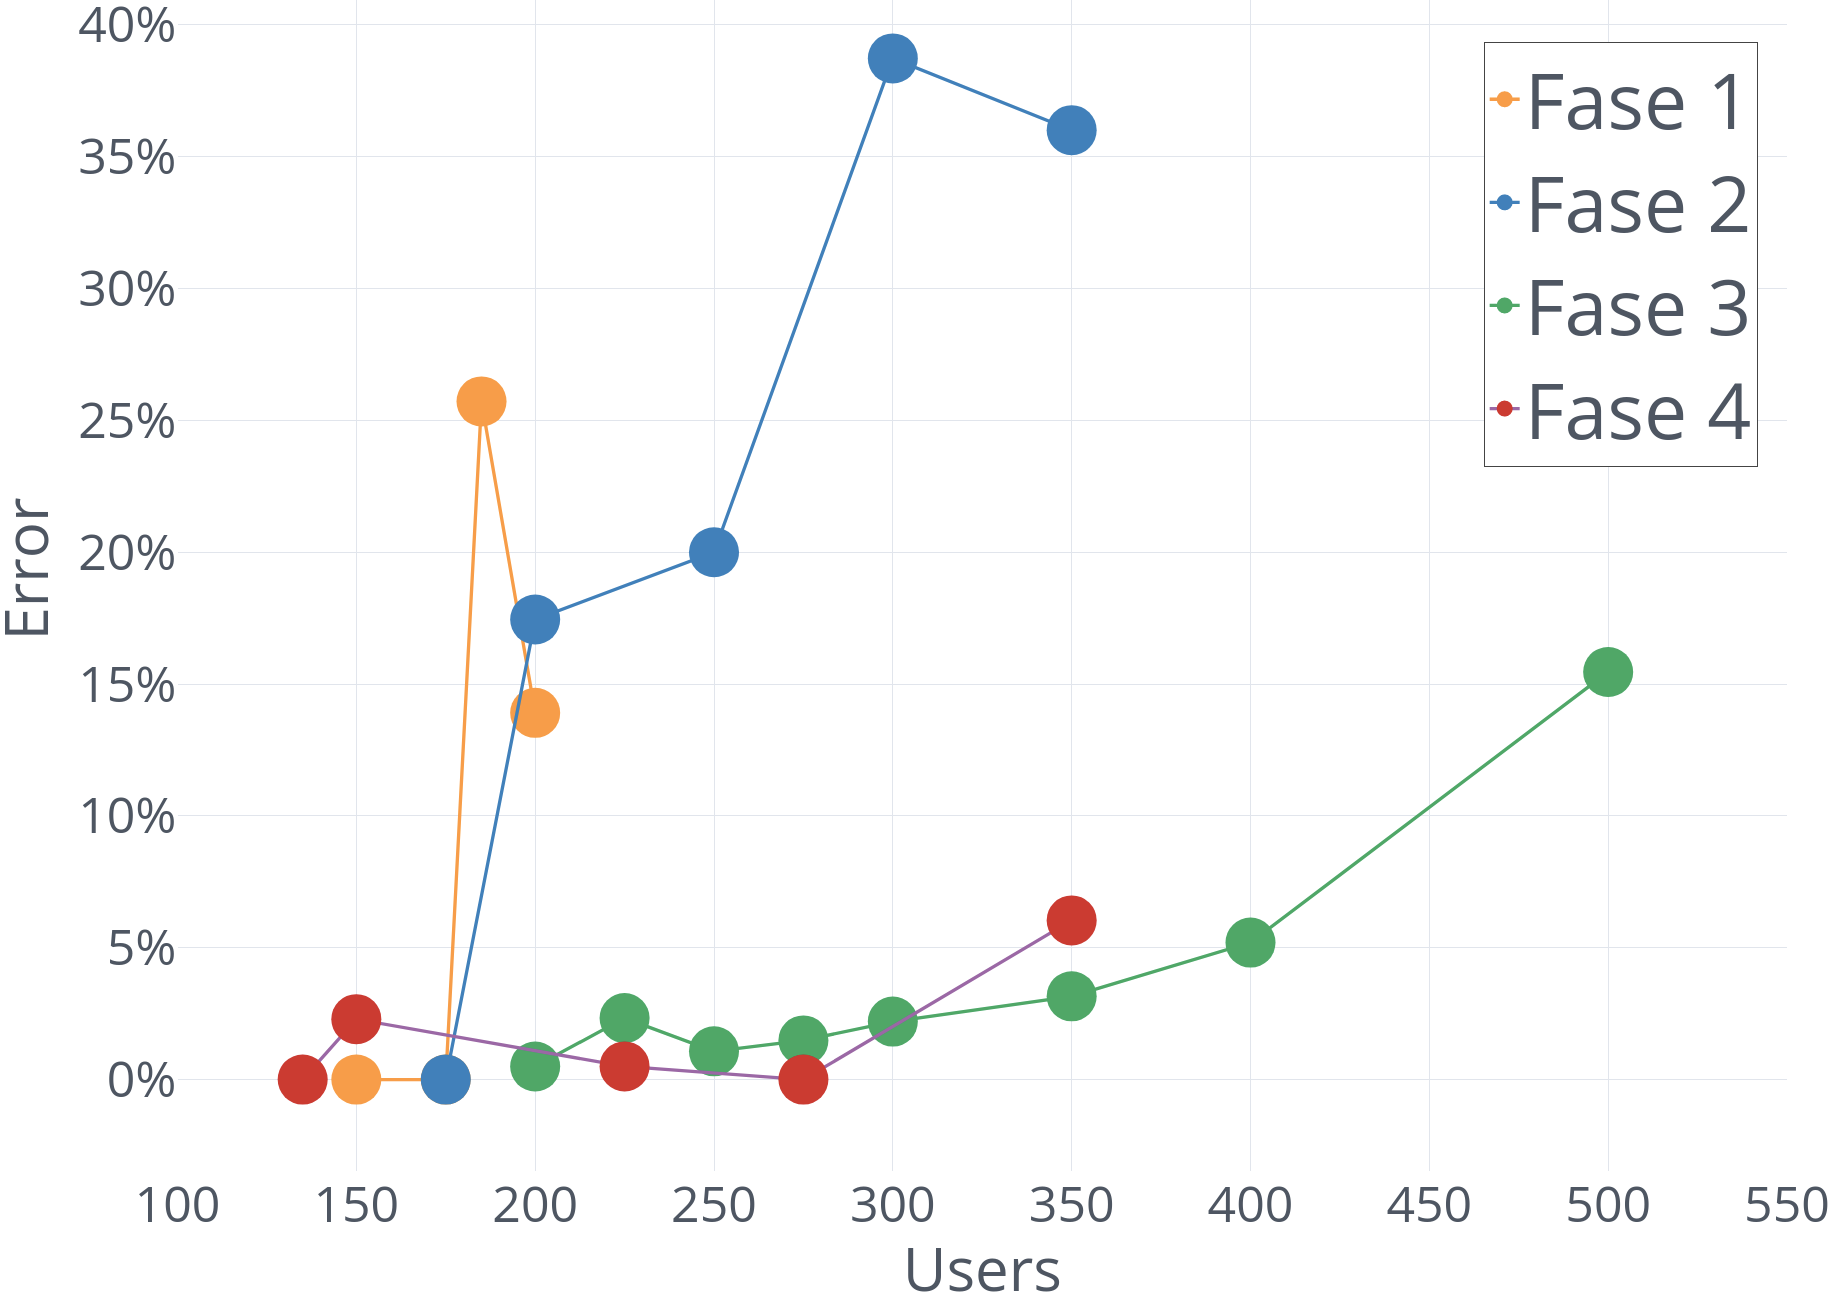
\includegraphics[width=1\linewidth]{Chapters/img/testing/1Pod.png} 
    \caption{One Pod} 
    \label{fig:1pod}
    \vspace{1ex}
  \end{minipage}%%
  \begin{minipage}[b]{0.5\linewidth}
    \centering
    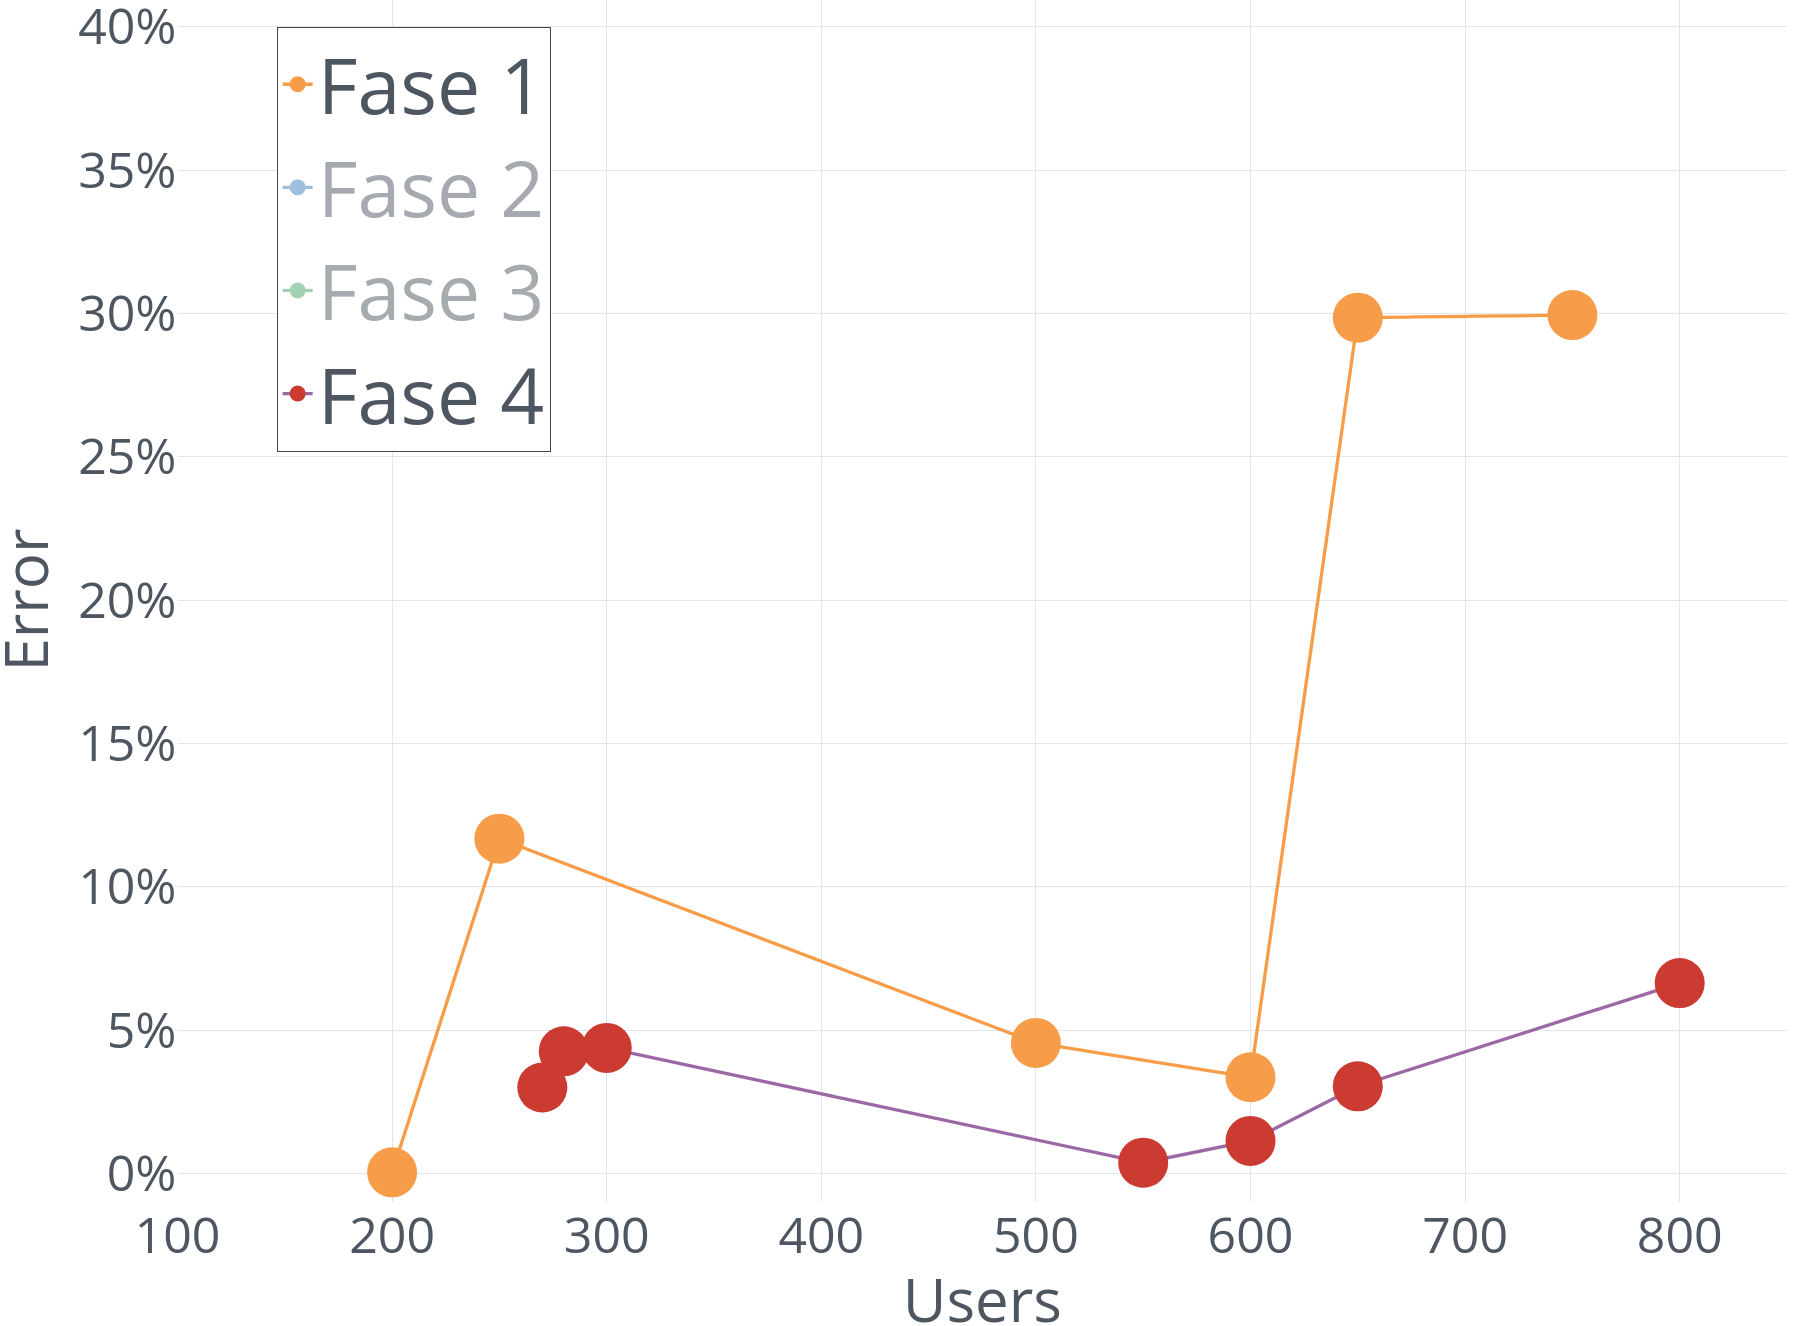
\includegraphics[width=1\linewidth]{Chapters/img/testing/2Pod.png} 
    \caption{Two Pods} 
    \label{fig:2pods}
    \vspace{1ex}
  \end{minipage} 
\end{figure}

The \textbf{first testing phase}, represented in orange, allowed us to understand that abundant resources would not suffice as the results were subpar, with an error rate above 10\% for 200 concurrent users. In this test, the pods were setup with 800 \acrfull{m} of CPU and 800 \acrfull{mib} of RAM.

During this phase, it was possible to observe that only 50\% of the pod memory was being utilized, so during \textbf{phase two (blue)}, we increase \acrshort{jvm} memory options to access 75\% of the available RAM. The change ended up with not affecting the error rate, proving that just adding more resources would not solve the problem, however it allowed for resource optimization, saving scarce resources.

From the previous tests, we came to the conclusion that the ideal memory values would be 400MB for the \acrshort{jvm}, from the 500\acrshort{mib} provided to the pod. With the ideal memory values found, we could now try to optimize the CPU which was given access to 1 entire core per pod, decreasing the error rate to below 5\% for 200 and 350 users, as can be observed in Fig. \ref{fig:1pod} during \textbf{phase three (green)}. This change also had an effect in the boot speed, which decreased from 50 seconds to an average of 30 seconds, and led us to test how different CPU resources affect boot speed.

All microservices were written in \textbf{Java} and include the \textbf{Spring} framework, which on average (observed from our services in idle), require about 120-200 \acrfull{mib} while online, with the most demanding ones using 500 \acrshort{mib} at peak load. The most problematic aspect when dealing with Spring is the boot time, strongly affected by the amount of CPU allocated to it. By testing, we were able to gather the following results, displayed on table \ref{tbl:cpuBoot}.

\begin{table}[!h]
    \centering
    \begin{tabular}{c|c}
    CPU (cores) & Boot (sec)  \\ \hline
    500m        & $\sim$120 \\
    800m        & $\sim$70  \\
    1000m       & $\sim$30 
    \end{tabular}
    
    \caption{Relation between processing power (CPU) and boot time}
    \label{tbl:cpuBoot}
\end{table}

As \acrshort{k8s} does not hoard the resources if not in use, as long as not explicitly told to do so, we decided to allow each pod access to one entire core. This way, we have resources for a fast boot, while also not wasting resources when they are idle as CPU usage is reduced to about 10 \acrshort{m}.

Still during phase three we have noticed that after booting up, the pods were using 300\acrshort{mib} of RAM that would slowly increase until running out of memory and crashing. To try and fix it, we experimented with a different garbage collector Garbage First Garbage Collector (G1GC), which actually started releasing memory when it was no longer necessary, increasing the pod uptime and error rate, observed in \textbf{phase four (red)}.

This phase provided the best results with \textbf{275 users with a 0\% error rate}, upon completing this stress test and finding the limit of our pod, we could now proceed with the next round of tests, where we try out the optimal configurations found for the pods. Which resulted in phase four (red) in Fig. \ref{fig:2pods}, which was an improvement over its phase one results allowing up to \textbf{600 users with a sub 2\% error rate}.

With the ideal pod configuration found and the pod user limits discovered, we can now focus on the scalability testing to understand how the system reacts to changes in the number of simultaneous users. The following metrics were chosen to test as scaling parameters:

\begin{enumerate}
    \item \textbf{http\_server\_requests\_seconds\_count} --- represents the number of requests received at a certain endpoint at a given time;
    \item \textbf{CPU usage} --- represents the CPU processing power being used at a given time;
    \item \textbf{http\_server\_requests\_seconds\_max} --- represents the maximum request duration during in a rolling window, as such the purpose is to measure the worst outlier, following the work of F. Rossi et al~\cite{rossi2020hierarchical}.
\end{enumerate}

And, as a way to optimize our solution, the following rules have been defined: 
It was also necessary to define some of the rules the system must follow, to ensure no resources were wasted and they fit within the findings discovered earlier in single pods testing.

\begin{itemize}
    \item Scaling up to two pods, only when the load is higher or similar to the ceiling found during our one pod test (e.g., should not scale with less than 200 users);
    \item The pods should be given a grace period to scale up, where they can handle the full load while the second pod is loading up without losing any requests;
    \item Handle almost the same load as the experiment that ran with two deployed pods.
\end{itemize}

\begin{figure}[h]
    \centering
    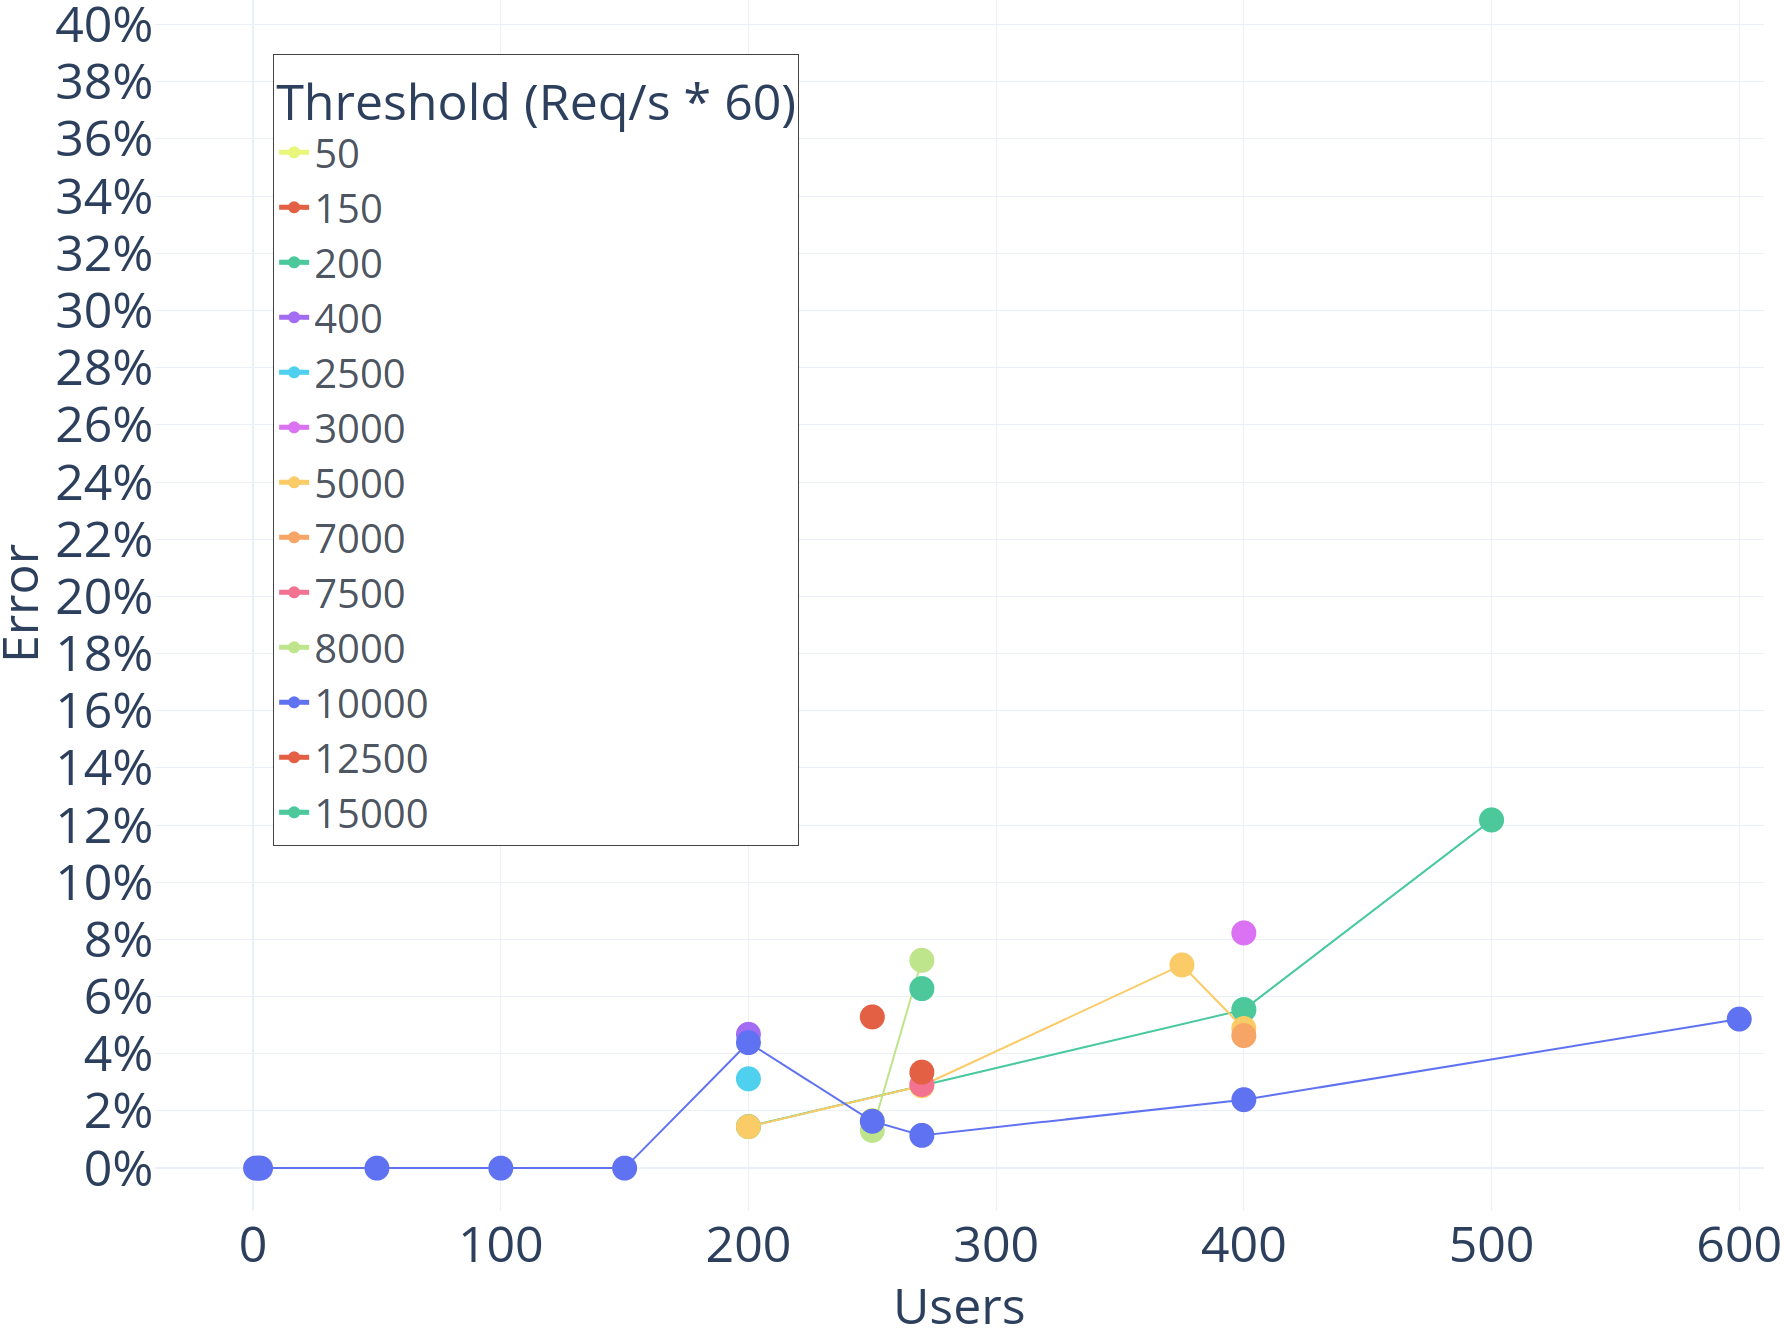
\includegraphics[width=0.5\textwidth]{Chapters/img/testing/HPA_HttpCountIncreaseLeft.png}
    \caption{Increase of HTTP Requests}
    \label{fig:metric_increase}
\end{figure}

As stated previously, the first metric tests a scenario where the system would scale based on the number of requests received, which can be seen in Fig. \ref{fig:metric_increase}. Over this metric, the Prometheus function \textbf{Increase} has been applied to a 1 minute window, which calculates the per-second average rate of increase of the time series in that interval and multiplies its value by the defined interval in seconds (60). In the mentioned figure, it is possible to observe that tests with more than 300 concurrent users had an error rate above 7.5\%, independent of the chosen threshold. In addition, we noticed that the pods were scaling even when below 200 concurrent users, breaking the first rule.

Despite the metric not meeting the defined requirements, it helped us realize that we were losing requests during the scaling period due to \acrshort{k8s} routing requests to newly instantiated pods. This happened because the pod was declared ready when \acrshort{jvm} launched, but not before Spring finished up booting up. To fix it, we had to swap the default implementations of the Readiness and Liveness probes, to the ones exposed through the Micrometer library. This way, pods are only declared ready and alive, when Spring is ready to process requests.

%Over the first metric, Fig.~\ref{fig:metric_increase}, the Prometheus function \textbf{Increase} has been applied with a 1 minute window, which calculates the per-second average rate of increase of the time series in that interval and multiplies its values by the defined interval in seconds (60). As seen in our figure, most of the tests with more than 300 users had an error rate above 7.5\%, independent of the chosen threshold. We also noticed that even when using values below 200 (way below our 1 pod threshold found previously), the pods would scale anyway, which violates one of our requirements. 

%Even though the metric didn't meet the defined requirements, it allowed us to realize that we were losing requests during the scaling period because Kubernetes was routing requests to the newly instantiated pod, as it was declared ready when JVM launched but before Spring finished booting up. We then implemented new readiness and liveness probes, based on the micrometer metrics, which allowed us to declare the pod as ready and alive only when Spring actually launches and is ready to process requests.

\begin{figure}[h]
    \centering
    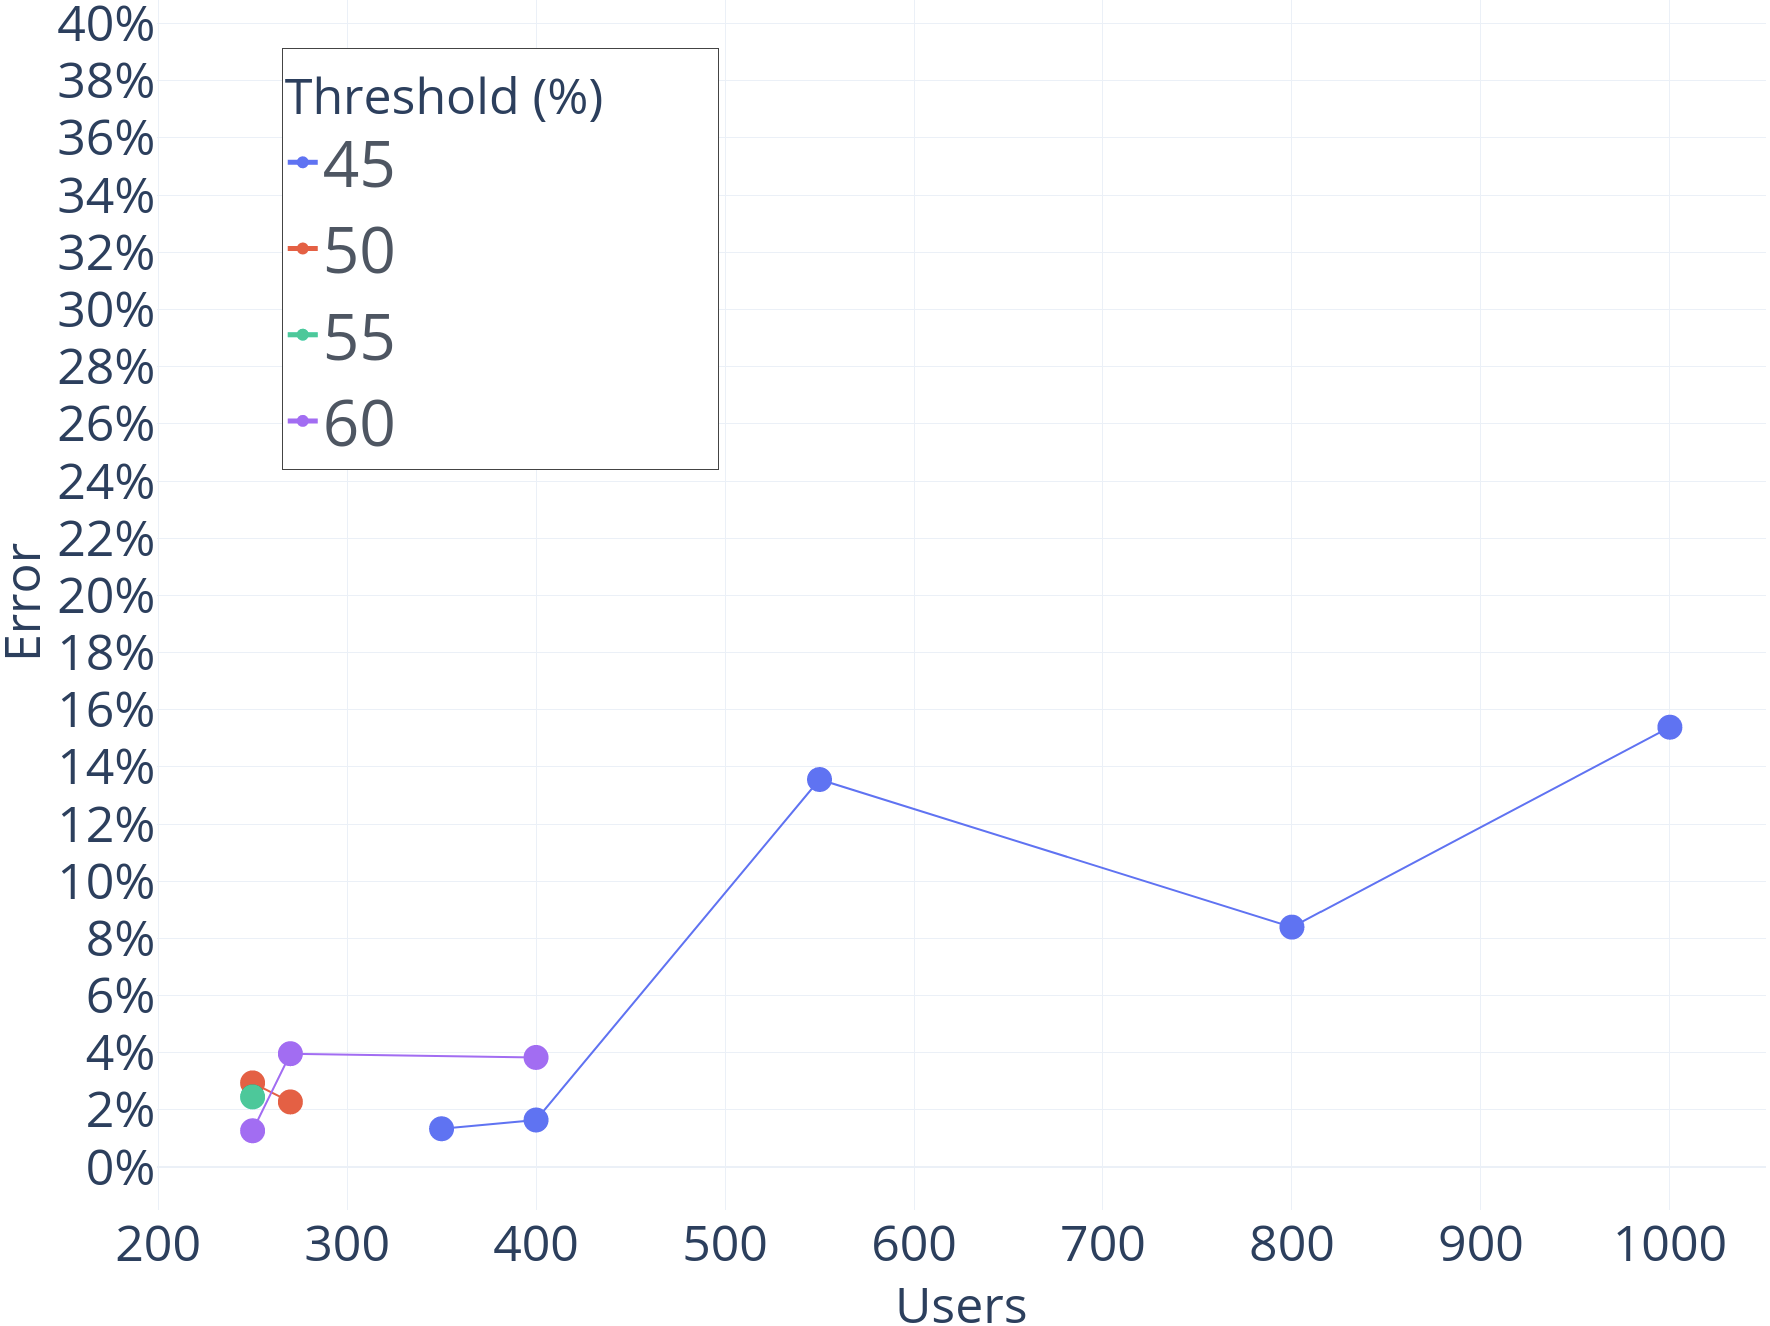
\includegraphics[width=0.5\textwidth]{Chapters/img/testing/HPA_CpuUsageLeft.png}
    \caption{Percentage of CPU usage}
    \label{fig:metric_cpu}
\end{figure}

For the second test, Fig. \ref{fig:metric_cpu}, the scaling was based on \textbf{CPU Usage}. We noticed that for the most part, the pod CPU usage was always at max load while receiving requests, which caused the cluster to immediately scale, independently of the number of concurrent users, explaining the poor results displayed.

%The second metric, \textbf{CPU usage} Fig.~\ref{fig:metric_cpu}, displayed poor results since CPU usage was for the most part, always at max load, which caused our cluster to immediately scale even though it was unnecessary. 

\begin{figure}[h]
    \centering
    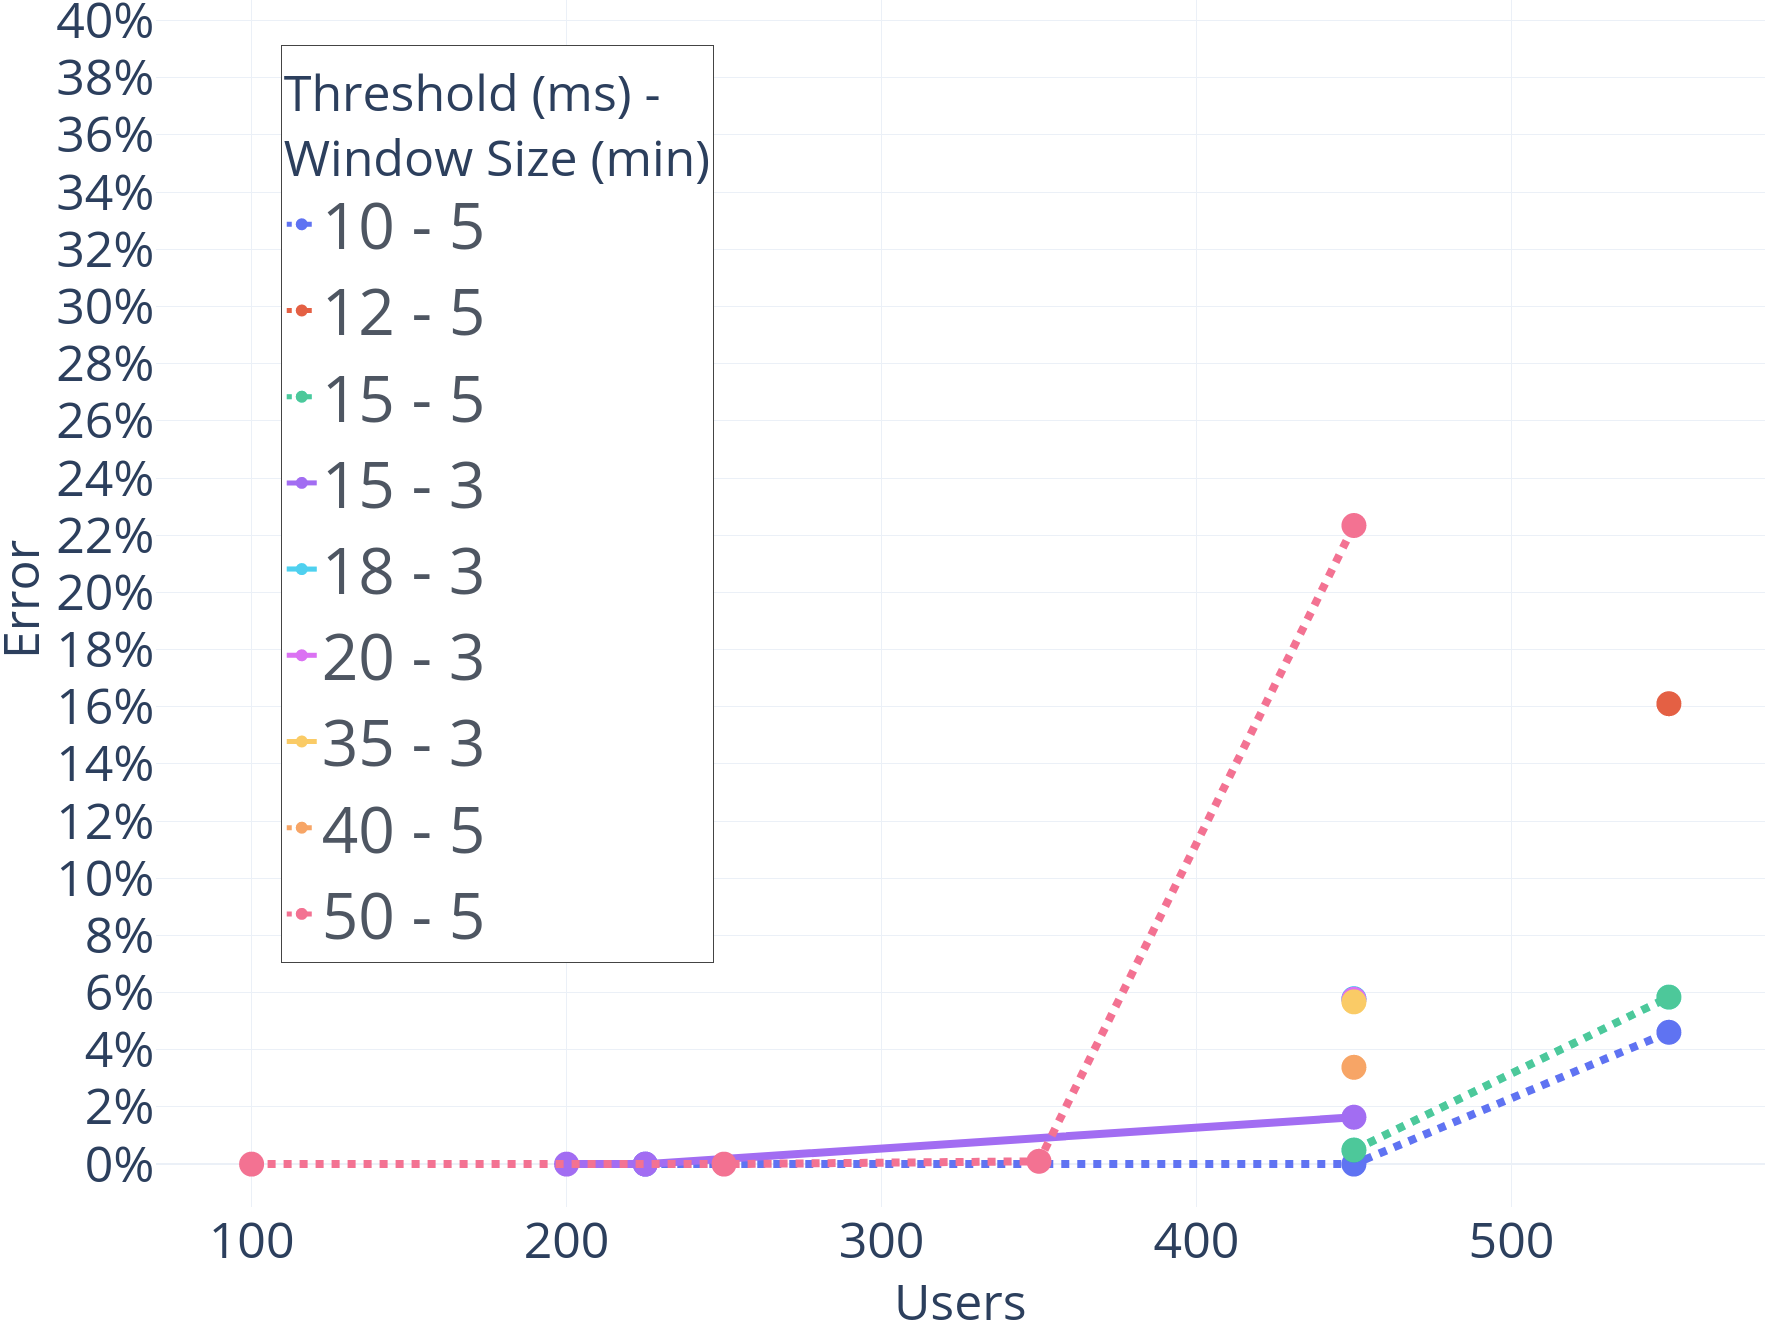
\includegraphics[width=0.5\textwidth]{Chapters/img/testing/HPA_HttpMaxRateLeft.png}
    \caption{Rate of MaxResponseTime}
    \label{fig:metric_max}
\end{figure}

For the final test, we experimented with \textbf{http\_server\_requests\_seconds\_max} extracted from the Micrometer library. On top of this data, we applied a Prometheus rate which calculates the per-second average rate of increase within a certain interval. We performed tests with 3 and 5 minute window intervals as observer in Fig. \ref{fig:metric_max}, with normal and dotted lines, respectively. 

In the same figure it is possible to observe that the 5 minute window produces good results, but, similarly to the results of the first metric, it would scale even when below the 200 users threshold, breaking our defined rule. Additionally, given the window size of the rate function, adjusting the threshold would not help as the test would be over by the time it would stabilize.

As such, we tried reducing the window to 3 minutes and increase the threshold to 50 to try and avoid unnecessary scaling, which backfired by never scaling, even when above 400 concurrent users. Trying different thresholds (40, 35, 20 and 18) while maintaining the same number of users (450) produced results by progressively decreasing the error rate to below 5\%, but still above the desired value of 2\%.

Based on these results, it led us to the 15ms threshold, where it managed to hold a \textbf{sub 2\% error rate with 450 users} and sustain, at least, 200 concurrent users without triggering the scaling process. As a final experiment, to confirm the results, the test duration was increased to 10 minutes and it managed to maintain the same error rate.






%\subsubsection{Scalability}
%\label{ss:scalability}

%\subsubsection{Load}
%\label{ss:load}

%\subsection{Usability}
%\label{s:usability}

%\todo[inline]{Fazer testes de usabilidade da aplicação com 15 a 30 pessoas}
%\todo[inline]{Avaliar eficácia do sistema de recomendaçoes}

% Fazer testes de usabilidade da aplicação com 15 a 30 pessoas
% Avaliar eficácia do sistema de recomendaçõe